\documentclass[twoside]{book}

% Packages required by doxygen
\usepackage{calc}
\usepackage{doxygen}
\usepackage{graphicx}
\usepackage[utf8]{inputenc}
\usepackage{makeidx}
\usepackage{multicol}
\usepackage{multirow}
\usepackage{textcomp}
\usepackage[table]{xcolor}

% Font selection
\usepackage[T1]{fontenc}
\usepackage{mathptmx}
\usepackage[scaled=.90]{helvet}
\usepackage{courier}
\usepackage{amssymb}
\usepackage{sectsty}
\renewcommand{\familydefault}{\sfdefault}
\allsectionsfont{%
  \fontseries{bc}\selectfont%
  \color{darkgray}%
}
\renewcommand{\DoxyLabelFont}{%
  \fontseries{bc}\selectfont%
  \color{darkgray}%
}

% Page & text layout
\usepackage{geometry}
\geometry{%
  a4paper,%
  top=2.5cm,%
  bottom=2.5cm,%
  left=2.5cm,%
  right=2.5cm%
}
\tolerance=750
\hfuzz=15pt
\hbadness=750
\setlength{\emergencystretch}{15pt}
\setlength{\parindent}{0cm}
\setlength{\parskip}{0.2cm}
\makeatletter
\renewcommand{\paragraph}{%
  \@startsection{paragraph}{4}{0ex}{-1.0ex}{1.0ex}{%
    \normalfont\normalsize\bfseries\SS@parafont%
  }%
}
\renewcommand{\subparagraph}{%
  \@startsection{subparagraph}{5}{0ex}{-1.0ex}{1.0ex}{%
    \normalfont\normalsize\bfseries\SS@subparafont%
  }%
}
\makeatother

% Headers & footers
\usepackage{fancyhdr}
\pagestyle{fancyplain}
\fancyhead[LE]{\fancyplain{}{\bfseries\thepage}}
\fancyhead[CE]{\fancyplain{}{}}
\fancyhead[RE]{\fancyplain{}{\bfseries\leftmark}}
\fancyhead[LO]{\fancyplain{}{\bfseries\rightmark}}
\fancyhead[CO]{\fancyplain{}{}}
\fancyhead[RO]{\fancyplain{}{\bfseries\thepage}}
\fancyfoot[LE]{\fancyplain{}{}}
\fancyfoot[CE]{\fancyplain{}{}}
\fancyfoot[RE]{\fancyplain{}{\bfseries\scriptsize Generated on Mon May 9 2016 09\-:34\-:14 for I\-J\-Engine by Doxygen }}
\fancyfoot[LO]{\fancyplain{}{\bfseries\scriptsize Generated on Mon May 9 2016 09\-:34\-:14 for I\-J\-Engine by Doxygen }}
\fancyfoot[CO]{\fancyplain{}{}}
\fancyfoot[RO]{\fancyplain{}{}}
\renewcommand{\footrulewidth}{0.4pt}
\renewcommand{\chaptermark}[1]{%
  \markboth{#1}{}%
}
\renewcommand{\sectionmark}[1]{%
  \markright{\thesection\ #1}%
}

% Indices & bibliography
\usepackage{natbib}
\usepackage[titles]{tocloft}
\setcounter{tocdepth}{3}
\setcounter{secnumdepth}{5}
\makeindex

% Hyperlinks (required, but should be loaded last)
\usepackage{ifpdf}
\ifpdf
  \usepackage[pdftex,pagebackref=true]{hyperref}
\else
  \usepackage[ps2pdf,pagebackref=true]{hyperref}
\fi
\hypersetup{%
  colorlinks=true,%
  linkcolor=blue,%
  citecolor=blue,%
  unicode%
}

% Custom commands
\newcommand{\clearemptydoublepage}{%
  \newpage{\pagestyle{empty}\cleardoublepage}%
}


%===== C O N T E N T S =====

\begin{document}

% Titlepage & ToC
\hypersetup{pageanchor=false}
\pagenumbering{roman}
\begin{titlepage}
\vspace*{7cm}
\begin{center}%
{\Large I\-J\-Engine }\\
\vspace*{1cm}
{\large Generated by Doxygen 1.8.6}\\
\vspace*{0.5cm}
{\small Mon May 9 2016 09:34:14}\\
\end{center}
\end{titlepage}
\clearemptydoublepage
\tableofcontents
\clearemptydoublepage
\pagenumbering{arabic}
\hypersetup{pageanchor=true}

%--- Begin generated contents ---
\chapter{Namespace Index}
\section{Namespace List}
Here is a list of all namespaces with brief descriptions\-:\begin{DoxyCompactList}
\item\contentsline{section}{\hyperlink{namespaceijengine}{ijengine} }{\pageref{namespaceijengine}}{}
\end{DoxyCompactList}

\chapter{Hierarchical Index}
\section{Class Hierarchy}
This inheritance list is sorted roughly, but not completely, alphabetically\-:\begin{DoxyCompactList}
\item \contentsline{section}{ijengine\-:\-:Canvas}{\pageref{classijengine_1_1Canvas}}{}
\begin{DoxyCompactList}
\item \contentsline{section}{ijengine\-:\-:S\-D\-L2\-Canvas}{\pageref{classijengine_1_1SDL2Canvas}}{}
\end{DoxyCompactList}
\item \contentsline{section}{ijengine\-:\-:Context\-Info}{\pageref{structijengine_1_1ContextInfo}}{}
\item \contentsline{section}{ijengine\-:\-:Framebuffer\-Info}{\pageref{structijengine_1_1FramebufferInfo}}{}
\item \contentsline{section}{ijengine\-:\-:Game}{\pageref{classijengine_1_1Game}}{}
\begin{DoxyCompactList}
\item \contentsline{section}{ijengine\-:\-:S\-D\-L2\-Game}{\pageref{classijengine_1_1SDL2Game}}{}
\item \contentsline{section}{ijengine\-:\-:S\-D\-L\-G\-L\-Game}{\pageref{classijengine_1_1SDLGLGame}}{}
\end{DoxyCompactList}
\item \contentsline{section}{ijengine\-:\-:Game\-Models}{\pageref{classijengine_1_1GameModels}}{}
\item I\-Game\-Object\begin{DoxyCompactList}
\item \contentsline{section}{ijengine\-:\-:Model}{\pageref{structijengine_1_1Model}}{}
\end{DoxyCompactList}
\item \contentsline{section}{ijengine\-:\-:Lib}{\pageref{classijengine_1_1Lib}}{}
\begin{DoxyCompactList}
\item \contentsline{section}{ijengine\-:\-:Lib\-G\-L}{\pageref{classijengine_1_1LibGL}}{}
\item \contentsline{section}{ijengine\-:\-:Lib\-S\-D\-L2}{\pageref{classijengine_1_1LibSDL2}}{}
\end{DoxyCompactList}
\item \contentsline{section}{ijengine\-:\-:Renderer3d}{\pageref{classijengine_1_1Renderer3d}}{}
\begin{DoxyCompactList}
\item \contentsline{section}{G\-Lrenderer3d}{\pageref{classGLrenderer3d}}{}
\end{DoxyCompactList}
\item \contentsline{section}{ijengine\-:\-:Shader\-Loader}{\pageref{classijengine_1_1ShaderLoader}}{}
\item \contentsline{section}{ijengine\-:\-:Shader\-Manager}{\pageref{classijengine_1_1ShaderManager}}{}
\item \contentsline{section}{ijengine\-:\-:Texture}{\pageref{classijengine_1_1Texture}}{}
\begin{DoxyCompactList}
\item \contentsline{section}{ijengine\-:\-:S\-D\-L2\-Texture}{\pageref{classijengine_1_1SDL2Texture}}{}
\end{DoxyCompactList}
\item \contentsline{section}{ijengine\-:\-:Vector3f}{\pageref{structijengine_1_1Vector3f}}{}
\item \contentsline{section}{ijengine\-:\-:Video}{\pageref{classijengine_1_1Video}}{}
\begin{DoxyCompactList}
\item \contentsline{section}{ijengine\-:\-:S\-D\-L2\-D\-Video}{\pageref{classijengine_1_1SDL2DVideo}}{}
\item \contentsline{section}{ijengine\-:\-:S\-D\-L3\-D\-Video}{\pageref{classijengine_1_1SDL3DVideo}}{}
\end{DoxyCompactList}
\item \contentsline{section}{ijengine\-:\-:Window}{\pageref{classijengine_1_1Window}}{}
\begin{DoxyCompactList}
\item \contentsline{section}{ijengine\-:\-:S\-D\-L2\-Window}{\pageref{classijengine_1_1SDL2Window}}{}
\end{DoxyCompactList}
\end{DoxyCompactList}

\chapter{Class Index}
\section{Class List}
Here are the classes, structs, unions and interfaces with brief descriptions\-:\begin{DoxyCompactList}
\item\contentsline{section}{\hyperlink{classijengine_1_1Canvas}{ijengine\-::\-Canvas} }{\pageref{classijengine_1_1Canvas}}{}
\item\contentsline{section}{\hyperlink{structijengine_1_1ContextInfo}{ijengine\-::\-Context\-Info} }{\pageref{structijengine_1_1ContextInfo}}{}
\item\contentsline{section}{\hyperlink{structijengine_1_1FramebufferInfo}{ijengine\-::\-Framebuffer\-Info} }{\pageref{structijengine_1_1FramebufferInfo}}{}
\item\contentsline{section}{\hyperlink{classijengine_1_1Game}{ijengine\-::\-Game} }{\pageref{classijengine_1_1Game}}{}
\item\contentsline{section}{\hyperlink{classijengine_1_1GameModels}{ijengine\-::\-Game\-Models} }{\pageref{classijengine_1_1GameModels}}{}
\item\contentsline{section}{\hyperlink{classGLrenderer3d}{G\-Lrenderer3d} }{\pageref{classGLrenderer3d}}{}
\item\contentsline{section}{\hyperlink{classijengine_1_1Lib}{ijengine\-::\-Lib} }{\pageref{classijengine_1_1Lib}}{}
\item\contentsline{section}{\hyperlink{classijengine_1_1LibGL}{ijengine\-::\-Lib\-G\-L} }{\pageref{classijengine_1_1LibGL}}{}
\item\contentsline{section}{\hyperlink{classijengine_1_1LibSDL2}{ijengine\-::\-Lib\-S\-D\-L2} }{\pageref{classijengine_1_1LibSDL2}}{}
\item\contentsline{section}{\hyperlink{structijengine_1_1Model}{ijengine\-::\-Model} }{\pageref{structijengine_1_1Model}}{}
\item\contentsline{section}{\hyperlink{classijengine_1_1Renderer3d}{ijengine\-::\-Renderer3d} }{\pageref{classijengine_1_1Renderer3d}}{}
\item\contentsline{section}{\hyperlink{classijengine_1_1SDL2Canvas}{ijengine\-::\-S\-D\-L2\-Canvas} }{\pageref{classijengine_1_1SDL2Canvas}}{}
\item\contentsline{section}{\hyperlink{classijengine_1_1SDL2DVideo}{ijengine\-::\-S\-D\-L2\-D\-Video} }{\pageref{classijengine_1_1SDL2DVideo}}{}
\item\contentsline{section}{\hyperlink{classijengine_1_1SDL2Game}{ijengine\-::\-S\-D\-L2\-Game} }{\pageref{classijengine_1_1SDL2Game}}{}
\item\contentsline{section}{\hyperlink{classijengine_1_1SDL2Texture}{ijengine\-::\-S\-D\-L2\-Texture} }{\pageref{classijengine_1_1SDL2Texture}}{}
\item\contentsline{section}{\hyperlink{classijengine_1_1SDL2Window}{ijengine\-::\-S\-D\-L2\-Window} }{\pageref{classijengine_1_1SDL2Window}}{}
\item\contentsline{section}{\hyperlink{classijengine_1_1SDL3DVideo}{ijengine\-::\-S\-D\-L3\-D\-Video} }{\pageref{classijengine_1_1SDL3DVideo}}{}
\item\contentsline{section}{\hyperlink{classijengine_1_1SDLGLGame}{ijengine\-::\-S\-D\-L\-G\-L\-Game} }{\pageref{classijengine_1_1SDLGLGame}}{}
\item\contentsline{section}{\hyperlink{classijengine_1_1ShaderLoader}{ijengine\-::\-Shader\-Loader} }{\pageref{classijengine_1_1ShaderLoader}}{}
\item\contentsline{section}{\hyperlink{classijengine_1_1ShaderManager}{ijengine\-::\-Shader\-Manager} }{\pageref{classijengine_1_1ShaderManager}}{}
\item\contentsline{section}{\hyperlink{classijengine_1_1Texture}{ijengine\-::\-Texture} }{\pageref{classijengine_1_1Texture}}{}
\item\contentsline{section}{\hyperlink{structijengine_1_1Vector3f}{ijengine\-::\-Vector3f} }{\pageref{structijengine_1_1Vector3f}}{}
\item\contentsline{section}{\hyperlink{classijengine_1_1Video}{ijengine\-::\-Video} }{\pageref{classijengine_1_1Video}}{}
\item\contentsline{section}{\hyperlink{classijengine_1_1Window}{ijengine\-::\-Window} }{\pageref{classijengine_1_1Window}}{}
\end{DoxyCompactList}

\chapter{File Index}
\section{File List}
Here is a list of all files with brief descriptions\-:\begin{DoxyCompactList}
\item\contentsline{section}{/home/carla/git/ijengine-\/\-I\-C\-G\-\_\-\-G\-L/include/\hyperlink{canvas_8h}{canvas.\-h} }{\pageref{canvas_8h}}{}
\item\contentsline{section}{/home/carla/git/ijengine-\/\-I\-C\-G\-\_\-\-G\-L/include/\hyperlink{contextinfo_8h}{contextinfo.\-h} }{\pageref{contextinfo_8h}}{}
\item\contentsline{section}{/home/carla/git/ijengine-\/\-I\-C\-G\-\_\-\-G\-L/include/\hyperlink{framebufferinfo_8h}{framebufferinfo.\-h} }{\pageref{framebufferinfo_8h}}{}
\item\contentsline{section}{/home/carla/git/ijengine-\/\-I\-C\-G\-\_\-\-G\-L/include/\hyperlink{game_8h}{game.\-h} }{\pageref{game_8h}}{}
\item\contentsline{section}{/home/carla/git/ijengine-\/\-I\-C\-G\-\_\-\-G\-L/include/\hyperlink{gamemodels_8h}{gamemodels.\-h} }{\pageref{gamemodels_8h}}{}
\item\contentsline{section}{/home/carla/git/ijengine-\/\-I\-C\-G\-\_\-\-G\-L/include/\hyperlink{glrenderer3d_8h}{glrenderer3d.\-h} }{\pageref{glrenderer3d_8h}}{}
\item\contentsline{section}{/home/carla/git/ijengine-\/\-I\-C\-G\-\_\-\-G\-L/include/\hyperlink{Igameobject_8h}{Igameobject.\-h} }{\pageref{Igameobject_8h}}{}
\item\contentsline{section}{/home/carla/git/ijengine-\/\-I\-C\-G\-\_\-\-G\-L/include/\hyperlink{libgl_8h}{libgl.\-h} }{\pageref{libgl_8h}}{}
\item\contentsline{section}{/home/carla/git/ijengine-\/\-I\-C\-G\-\_\-\-G\-L/include/\hyperlink{libs_8h}{libs.\-h} }{\pageref{libs_8h}}{}
\item\contentsline{section}{/home/carla/git/ijengine-\/\-I\-C\-G\-\_\-\-G\-L/include/\hyperlink{model_8h}{model.\-h} }{\pageref{model_8h}}{}
\item\contentsline{section}{/home/carla/git/ijengine-\/\-I\-C\-G\-\_\-\-G\-L/include/\hyperlink{renderer3d_8h}{renderer3d.\-h} }{\pageref{renderer3d_8h}}{}
\item\contentsline{section}{/home/carla/git/ijengine-\/\-I\-C\-G\-\_\-\-G\-L/include/\hyperlink{sdl2_8h}{sdl2.\-h} }{\pageref{sdl2_8h}}{}
\item\contentsline{section}{/home/carla/git/ijengine-\/\-I\-C\-G\-\_\-\-G\-L/include/\hyperlink{sdl2canvas_8h}{sdl2canvas.\-h} }{\pageref{sdl2canvas_8h}}{}
\item\contentsline{section}{/home/carla/git/ijengine-\/\-I\-C\-G\-\_\-\-G\-L/include/\hyperlink{sdl2Dvideo_8h}{sdl2\-Dvideo.\-h} }{\pageref{sdl2Dvideo_8h}}{}
\item\contentsline{section}{/home/carla/git/ijengine-\/\-I\-C\-G\-\_\-\-G\-L/include/\hyperlink{sdl2game_8h}{sdl2game.\-h} }{\pageref{sdl2game_8h}}{}
\item\contentsline{section}{/home/carla/git/ijengine-\/\-I\-C\-G\-\_\-\-G\-L/include/\hyperlink{sdl2texture_8h}{sdl2texture.\-h} }{\pageref{sdl2texture_8h}}{}
\item\contentsline{section}{/home/carla/git/ijengine-\/\-I\-C\-G\-\_\-\-G\-L/include/\hyperlink{sdl2window_8h}{sdl2window.\-h} }{\pageref{sdl2window_8h}}{}
\item\contentsline{section}{/home/carla/git/ijengine-\/\-I\-C\-G\-\_\-\-G\-L/include/\hyperlink{sdl3Dvideo_8h}{sdl3\-Dvideo.\-h} }{\pageref{sdl3Dvideo_8h}}{}
\item\contentsline{section}{/home/carla/git/ijengine-\/\-I\-C\-G\-\_\-\-G\-L/include/\hyperlink{sdlglgame_8h}{sdlglgame.\-h} }{\pageref{sdlglgame_8h}}{}
\item\contentsline{section}{/home/carla/git/ijengine-\/\-I\-C\-G\-\_\-\-G\-L/include/\hyperlink{shader__manager_8h}{shader\-\_\-manager.\-h} }{\pageref{shader__manager_8h}}{}
\item\contentsline{section}{/home/carla/git/ijengine-\/\-I\-C\-G\-\_\-\-G\-L/include/\hyperlink{shaderloader_8h}{shaderloader.\-h} }{\pageref{shaderloader_8h}}{}
\item\contentsline{section}{/home/carla/git/ijengine-\/\-I\-C\-G\-\_\-\-G\-L/include/\hyperlink{texture_8h}{texture.\-h} }{\pageref{texture_8h}}{}
\item\contentsline{section}{/home/carla/git/ijengine-\/\-I\-C\-G\-\_\-\-G\-L/include/\hyperlink{vertexformat_8h}{vertexformat.\-h} }{\pageref{vertexformat_8h}}{}
\item\contentsline{section}{/home/carla/git/ijengine-\/\-I\-C\-G\-\_\-\-G\-L/include/\hyperlink{video_8h}{video.\-h} }{\pageref{video_8h}}{}
\item\contentsline{section}{/home/carla/git/ijengine-\/\-I\-C\-G\-\_\-\-G\-L/include/\hyperlink{window_8h}{window.\-h} }{\pageref{window_8h}}{}
\item\contentsline{section}{/home/carla/git/ijengine-\/\-I\-C\-G\-\_\-\-G\-L/src/\hyperlink{game_8cpp}{game.\-cpp} }{\pageref{game_8cpp}}{}
\item\contentsline{section}{/home/carla/git/ijengine-\/\-I\-C\-G\-\_\-\-G\-L/src/\hyperlink{glrenderer3d_8cpp}{glrenderer3d.\-cpp} }{\pageref{glrenderer3d_8cpp}}{}
\item\contentsline{section}{/home/carla/git/ijengine-\/\-I\-C\-G\-\_\-\-G\-L/src/\hyperlink{libgl_8cpp}{libgl.\-cpp} }{\pageref{libgl_8cpp}}{}
\item\contentsline{section}{/home/carla/git/ijengine-\/\-I\-C\-G\-\_\-\-G\-L/src/\hyperlink{sdl2_8cpp}{sdl2.\-cpp} }{\pageref{sdl2_8cpp}}{}
\item\contentsline{section}{/home/carla/git/ijengine-\/\-I\-C\-G\-\_\-\-G\-L/src/\hyperlink{sdl2canvas_8cpp}{sdl2canvas.\-cpp} }{\pageref{sdl2canvas_8cpp}}{}
\item\contentsline{section}{/home/carla/git/ijengine-\/\-I\-C\-G\-\_\-\-G\-L/src/\hyperlink{sdl2Dvideo_8cpp}{sdl2\-Dvideo.\-cpp} }{\pageref{sdl2Dvideo_8cpp}}{}
\item\contentsline{section}{/home/carla/git/ijengine-\/\-I\-C\-G\-\_\-\-G\-L/src/\hyperlink{sdl2game_8cpp}{sdl2game.\-cpp} }{\pageref{sdl2game_8cpp}}{}
\item\contentsline{section}{/home/carla/git/ijengine-\/\-I\-C\-G\-\_\-\-G\-L/src/\hyperlink{sdl2texture_8cpp}{sdl2texture.\-cpp} }{\pageref{sdl2texture_8cpp}}{}
\item\contentsline{section}{/home/carla/git/ijengine-\/\-I\-C\-G\-\_\-\-G\-L/src/\hyperlink{sdl2window_8cpp}{sdl2window.\-cpp} }{\pageref{sdl2window_8cpp}}{}
\item\contentsline{section}{/home/carla/git/ijengine-\/\-I\-C\-G\-\_\-\-G\-L/src/\hyperlink{sdl3Dvideo_8cpp}{sdl3\-Dvideo.\-cpp} }{\pageref{sdl3Dvideo_8cpp}}{}
\item\contentsline{section}{/home/carla/git/ijengine-\/\-I\-C\-G\-\_\-\-G\-L/src/\hyperlink{sdlglgame_8cpp}{sdlglgame.\-cpp} }{\pageref{sdlglgame_8cpp}}{}
\item\contentsline{section}{/home/carla/git/ijengine-\/\-I\-C\-G\-\_\-\-G\-L/src/\hyperlink{shader__manager_8cpp}{shader\-\_\-manager.\-cpp} }{\pageref{shader__manager_8cpp}}{}
\end{DoxyCompactList}

\chapter{Namespace Documentation}
\hypertarget{namespaceijengine}{\section{ijengine Namespace Reference}
\label{namespaceijengine}\index{ijengine@{ijengine}}
}
\subsection*{Classes}
\begin{DoxyCompactItemize}
\item 
class \hyperlink{classijengine_1_1Canvas}{Canvas}
\item 
struct \hyperlink{structijengine_1_1ContextInfo}{Context\-Info}
\item 
struct \hyperlink{structijengine_1_1FramebufferInfo}{Framebuffer\-Info}
\item 
class \hyperlink{classijengine_1_1Game}{Game}
\item 
class \hyperlink{structijengine_1_1Model}{Model}
\item 
class \hyperlink{classijengine_1_1GameModels}{Game\-Models}
\item 
class \hyperlink{classijengine_1_1LibGL}{Lib\-G\-L}
\item 
class \hyperlink{classijengine_1_1Lib}{Lib}
\item 
class \hyperlink{classijengine_1_1Renderer3d}{Renderer3d}
\item 
class \hyperlink{classijengine_1_1LibSDL2}{Lib\-S\-D\-L2}
\item 
class \hyperlink{classijengine_1_1SDL2Canvas}{S\-D\-L2\-Canvas}
\item 
class \hyperlink{classijengine_1_1SDL2DVideo}{S\-D\-L2\-D\-Video}
\item 
class \hyperlink{classijengine_1_1SDL2Game}{S\-D\-L2\-Game}
\item 
class \hyperlink{classijengine_1_1SDL2Texture}{S\-D\-L2\-Texture}
\item 
class \hyperlink{classijengine_1_1SDL2Window}{S\-D\-L2\-Window}
\item 
class \hyperlink{classijengine_1_1SDL3DVideo}{S\-D\-L3\-D\-Video}
\item 
class \hyperlink{classijengine_1_1SDLGLGame}{S\-D\-L\-G\-L\-Game}
\item 
class \hyperlink{classijengine_1_1ShaderManager}{Shader\-Manager}
\item 
class \hyperlink{classijengine_1_1ShaderLoader}{Shader\-Loader}
\item 
class \hyperlink{classijengine_1_1Texture}{Texture}
\item 
struct \hyperlink{structijengine_1_1Vector3f}{Vector3f}
\item 
class \hyperlink{classijengine_1_1Video}{Video}
\item 
class \hyperlink{classijengine_1_1Window}{Window}
\end{DoxyCompactItemize}

\chapter{Class Documentation}
\hypertarget{classijengine_1_1Canvas}{\section{ijengine\-:\-:Canvas Class Reference}
\label{classijengine_1_1Canvas}\index{ijengine\-::\-Canvas@{ijengine\-::\-Canvas}}
}


{\ttfamily \#include $<$canvas.\-h$>$}



Inheritance diagram for ijengine\-:\-:Canvas\-:\nopagebreak
\begin{figure}[H]
\begin{center}
\leavevmode
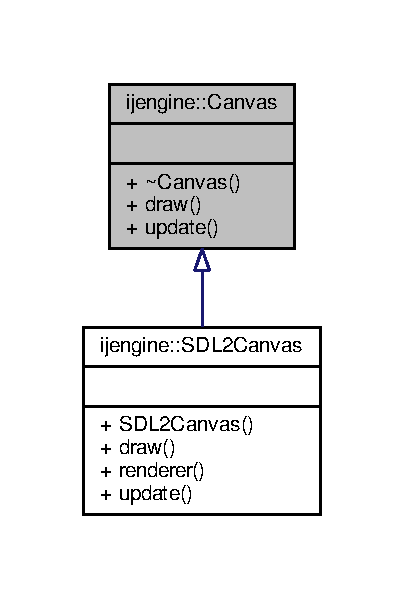
\includegraphics[width=194pt]{classijengine_1_1Canvas__inherit__graph}
\end{center}
\end{figure}


Collaboration diagram for ijengine\-:\-:Canvas\-:\nopagebreak
\begin{figure}[H]
\begin{center}
\leavevmode
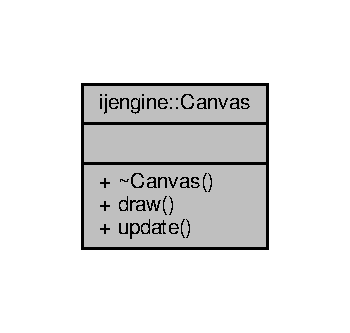
\includegraphics[width=168pt]{classijengine_1_1Canvas__coll__graph}
\end{center}
\end{figure}
\subsection*{Public Member Functions}
\begin{DoxyCompactItemize}
\item 
virtual \hyperlink{classijengine_1_1Canvas_a8ad1b6003932c8a359cc67d139e56b6f}{$\sim$\-Canvas} ()=default
\item 
virtual void \hyperlink{classijengine_1_1Canvas_ad941145373d040fa6b3b6f65366aaafa}{draw} (const \hyperlink{classijengine_1_1Texture}{Texture} $\ast$texture, int x, int y)=0
\item 
virtual void \hyperlink{classijengine_1_1Canvas_ad0f3aace5114a8cb2d457f0f272c6743}{update} ()=0
\end{DoxyCompactItemize}


\subsection{Constructor \& Destructor Documentation}
\hypertarget{classijengine_1_1Canvas_a8ad1b6003932c8a359cc67d139e56b6f}{\index{ijengine\-::\-Canvas@{ijengine\-::\-Canvas}!$\sim$\-Canvas@{$\sim$\-Canvas}}
\index{$\sim$\-Canvas@{$\sim$\-Canvas}!ijengine::Canvas@{ijengine\-::\-Canvas}}
\subsubsection[{$\sim$\-Canvas}]{\setlength{\rightskip}{0pt plus 5cm}virtual ijengine\-::\-Canvas\-::$\sim$\-Canvas (
\begin{DoxyParamCaption}
{}
\end{DoxyParamCaption}
)\hspace{0.3cm}{\ttfamily [virtual]}, {\ttfamily [default]}}}\label{classijengine_1_1Canvas_a8ad1b6003932c8a359cc67d139e56b6f}


\subsection{Member Function Documentation}
\hypertarget{classijengine_1_1Canvas_ad941145373d040fa6b3b6f65366aaafa}{\index{ijengine\-::\-Canvas@{ijengine\-::\-Canvas}!draw@{draw}}
\index{draw@{draw}!ijengine::Canvas@{ijengine\-::\-Canvas}}
\subsubsection[{draw}]{\setlength{\rightskip}{0pt plus 5cm}virtual void ijengine\-::\-Canvas\-::draw (
\begin{DoxyParamCaption}
\item[{const {\bf Texture} $\ast$}]{texture, }
\item[{int}]{x, }
\item[{int}]{y}
\end{DoxyParamCaption}
)\hspace{0.3cm}{\ttfamily [pure virtual]}}}\label{classijengine_1_1Canvas_ad941145373d040fa6b3b6f65366aaafa}


Implemented in \hyperlink{classijengine_1_1SDL2Canvas_a764abc16a5bcdd6f0d1ab1c117839ee0}{ijengine\-::\-S\-D\-L2\-Canvas}.

\hypertarget{classijengine_1_1Canvas_ad0f3aace5114a8cb2d457f0f272c6743}{\index{ijengine\-::\-Canvas@{ijengine\-::\-Canvas}!update@{update}}
\index{update@{update}!ijengine::Canvas@{ijengine\-::\-Canvas}}
\subsubsection[{update}]{\setlength{\rightskip}{0pt plus 5cm}virtual void ijengine\-::\-Canvas\-::update (
\begin{DoxyParamCaption}
{}
\end{DoxyParamCaption}
)\hspace{0.3cm}{\ttfamily [pure virtual]}}}\label{classijengine_1_1Canvas_ad0f3aace5114a8cb2d457f0f272c6743}


Implemented in \hyperlink{classijengine_1_1SDL2Canvas_a5b87afff98211d159da84986f5b04e99}{ijengine\-::\-S\-D\-L2\-Canvas}.



The documentation for this class was generated from the following file\-:\begin{DoxyCompactItemize}
\item 
/home/carla/git/ijengine-\/\-I\-C\-G\-\_\-\-G\-L/include/\hyperlink{canvas_8h}{canvas.\-h}\end{DoxyCompactItemize}

\hypertarget{structijengine_1_1ContextInfo}{\section{ijengine\-:\-:Context\-Info Struct Reference}
\label{structijengine_1_1ContextInfo}\index{ijengine\-::\-Context\-Info@{ijengine\-::\-Context\-Info}}
}


{\ttfamily \#include $<$contextinfo.\-h$>$}



Collaboration diagram for ijengine\-:\-:Context\-Info\-:\nopagebreak
\begin{figure}[H]
\begin{center}
\leavevmode
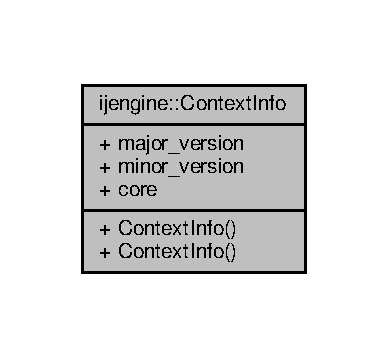
\includegraphics[width=186pt]{structijengine_1_1ContextInfo__coll__graph}
\end{center}
\end{figure}
\subsection*{Public Member Functions}
\begin{DoxyCompactItemize}
\item 
\hyperlink{structijengine_1_1ContextInfo_a82768f50efbf3d056282baffcbff66bd}{Context\-Info} ()
\item 
\hyperlink{structijengine_1_1ContextInfo_a7d8de4f7da93da958f06a1ef342f2c4c}{Context\-Info} (int majorversion, int minorversion, bool \-\_\-core)
\end{DoxyCompactItemize}
\subsection*{Public Attributes}
\begin{DoxyCompactItemize}
\item 
int \hyperlink{structijengine_1_1ContextInfo_a44c279f6a92cc71d0646efc13f20b925}{major\-\_\-version}
\item 
int \hyperlink{structijengine_1_1ContextInfo_a9027633774ff617b758c3be0ad456933}{minor\-\_\-version}
\item 
bool \hyperlink{structijengine_1_1ContextInfo_ae94af83cb75cdf9565ad810819d25351}{core}
\end{DoxyCompactItemize}


\subsection{Constructor \& Destructor Documentation}
\hypertarget{structijengine_1_1ContextInfo_a82768f50efbf3d056282baffcbff66bd}{\index{ijengine\-::\-Context\-Info@{ijengine\-::\-Context\-Info}!Context\-Info@{Context\-Info}}
\index{Context\-Info@{Context\-Info}!ijengine::ContextInfo@{ijengine\-::\-Context\-Info}}
\subsubsection[{Context\-Info}]{\setlength{\rightskip}{0pt plus 5cm}ijengine\-::\-Context\-Info\-::\-Context\-Info (
\begin{DoxyParamCaption}
{}
\end{DoxyParamCaption}
)\hspace{0.3cm}{\ttfamily [inline]}}}\label{structijengine_1_1ContextInfo_a82768f50efbf3d056282baffcbff66bd}
\hypertarget{structijengine_1_1ContextInfo_a7d8de4f7da93da958f06a1ef342f2c4c}{\index{ijengine\-::\-Context\-Info@{ijengine\-::\-Context\-Info}!Context\-Info@{Context\-Info}}
\index{Context\-Info@{Context\-Info}!ijengine::ContextInfo@{ijengine\-::\-Context\-Info}}
\subsubsection[{Context\-Info}]{\setlength{\rightskip}{0pt plus 5cm}ijengine\-::\-Context\-Info\-::\-Context\-Info (
\begin{DoxyParamCaption}
\item[{int}]{majorversion, }
\item[{int}]{minorversion, }
\item[{bool}]{\-\_\-core}
\end{DoxyParamCaption}
)\hspace{0.3cm}{\ttfamily [inline]}}}\label{structijengine_1_1ContextInfo_a7d8de4f7da93da958f06a1ef342f2c4c}


\subsection{Member Data Documentation}
\hypertarget{structijengine_1_1ContextInfo_ae94af83cb75cdf9565ad810819d25351}{\index{ijengine\-::\-Context\-Info@{ijengine\-::\-Context\-Info}!core@{core}}
\index{core@{core}!ijengine::ContextInfo@{ijengine\-::\-Context\-Info}}
\subsubsection[{core}]{\setlength{\rightskip}{0pt plus 5cm}bool ijengine\-::\-Context\-Info\-::core}}\label{structijengine_1_1ContextInfo_ae94af83cb75cdf9565ad810819d25351}
\hypertarget{structijengine_1_1ContextInfo_a44c279f6a92cc71d0646efc13f20b925}{\index{ijengine\-::\-Context\-Info@{ijengine\-::\-Context\-Info}!major\-\_\-version@{major\-\_\-version}}
\index{major\-\_\-version@{major\-\_\-version}!ijengine::ContextInfo@{ijengine\-::\-Context\-Info}}
\subsubsection[{major\-\_\-version}]{\setlength{\rightskip}{0pt plus 5cm}int ijengine\-::\-Context\-Info\-::major\-\_\-version}}\label{structijengine_1_1ContextInfo_a44c279f6a92cc71d0646efc13f20b925}
\hypertarget{structijengine_1_1ContextInfo_a9027633774ff617b758c3be0ad456933}{\index{ijengine\-::\-Context\-Info@{ijengine\-::\-Context\-Info}!minor\-\_\-version@{minor\-\_\-version}}
\index{minor\-\_\-version@{minor\-\_\-version}!ijengine::ContextInfo@{ijengine\-::\-Context\-Info}}
\subsubsection[{minor\-\_\-version}]{\setlength{\rightskip}{0pt plus 5cm}int ijengine\-::\-Context\-Info\-::minor\-\_\-version}}\label{structijengine_1_1ContextInfo_a9027633774ff617b758c3be0ad456933}


The documentation for this struct was generated from the following file\-:\begin{DoxyCompactItemize}
\item 
/home/carla/git/ijengine-\/\-I\-C\-G\-\_\-\-G\-L/include/\hyperlink{contextinfo_8h}{contextinfo.\-h}\end{DoxyCompactItemize}

\hypertarget{structijengine_1_1FramebufferInfo}{\section{ijengine\-:\-:Framebuffer\-Info Struct Reference}
\label{structijengine_1_1FramebufferInfo}\index{ijengine\-::\-Framebuffer\-Info@{ijengine\-::\-Framebuffer\-Info}}
}


{\ttfamily \#include $<$framebufferinfo.\-h$>$}



Collaboration diagram for ijengine\-:\-:Framebuffer\-Info\-:\nopagebreak
\begin{figure}[H]
\begin{center}
\leavevmode
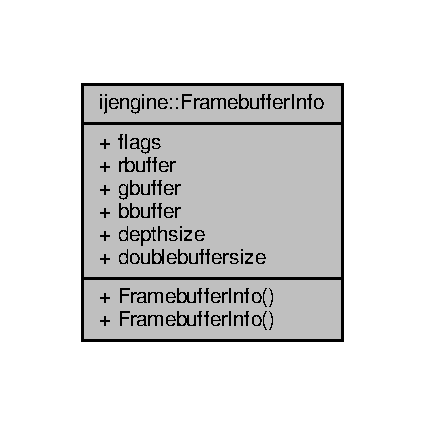
\includegraphics[width=204pt]{structijengine_1_1FramebufferInfo__coll__graph}
\end{center}
\end{figure}
\subsection*{Public Member Functions}
\begin{DoxyCompactItemize}
\item 
\hyperlink{structijengine_1_1FramebufferInfo_a507eb4b030e4818df4f4cf8591484fd0}{Framebuffer\-Info} ()
\item 
\hyperlink{structijengine_1_1FramebufferInfo_ab09fee22e3623d28a46cf8138d7b7761}{Framebuffer\-Info} (int r\-\_\-buffer\-\_\-size, int g\-\_\-buffer\-\_\-size, int b\-\_\-buffer\-\_\-size, int depth\-\_\-size, int double\-\_\-buffer\-\_\-size)
\end{DoxyCompactItemize}
\subsection*{Public Attributes}
\begin{DoxyCompactItemize}
\item 
unsigned int \hyperlink{structijengine_1_1FramebufferInfo_a7f874c6c0e1b04206adc6995e79926ff}{flags}
\item 
int \hyperlink{structijengine_1_1FramebufferInfo_aa8891e2879a75364bed1b6559ceaf575}{rbuffer} = 5
\item 
int \hyperlink{structijengine_1_1FramebufferInfo_a8e09a95dc7d365ac5cb77e5a87e876a0}{gbuffer} = 5
\item 
int \hyperlink{structijengine_1_1FramebufferInfo_ac434b7ef3cb86871cf42a943126b3d33}{bbuffer} = 5
\item 
int \hyperlink{structijengine_1_1FramebufferInfo_afb2371328a1647ebc4acc0757e825e9f}{depthsize} = 16
\item 
int \hyperlink{structijengine_1_1FramebufferInfo_a057843d29ea24330df32cacfdf8d79ea}{doublebuffersize} = 1
\end{DoxyCompactItemize}


\subsection{Constructor \& Destructor Documentation}
\hypertarget{structijengine_1_1FramebufferInfo_a507eb4b030e4818df4f4cf8591484fd0}{\index{ijengine\-::\-Framebuffer\-Info@{ijengine\-::\-Framebuffer\-Info}!Framebuffer\-Info@{Framebuffer\-Info}}
\index{Framebuffer\-Info@{Framebuffer\-Info}!ijengine::FramebufferInfo@{ijengine\-::\-Framebuffer\-Info}}
\subsubsection[{Framebuffer\-Info}]{\setlength{\rightskip}{0pt plus 5cm}ijengine\-::\-Framebuffer\-Info\-::\-Framebuffer\-Info (
\begin{DoxyParamCaption}
{}
\end{DoxyParamCaption}
)\hspace{0.3cm}{\ttfamily [inline]}}}\label{structijengine_1_1FramebufferInfo_a507eb4b030e4818df4f4cf8591484fd0}
\hypertarget{structijengine_1_1FramebufferInfo_ab09fee22e3623d28a46cf8138d7b7761}{\index{ijengine\-::\-Framebuffer\-Info@{ijengine\-::\-Framebuffer\-Info}!Framebuffer\-Info@{Framebuffer\-Info}}
\index{Framebuffer\-Info@{Framebuffer\-Info}!ijengine::FramebufferInfo@{ijengine\-::\-Framebuffer\-Info}}
\subsubsection[{Framebuffer\-Info}]{\setlength{\rightskip}{0pt plus 5cm}ijengine\-::\-Framebuffer\-Info\-::\-Framebuffer\-Info (
\begin{DoxyParamCaption}
\item[{int}]{r\-\_\-buffer\-\_\-size, }
\item[{int}]{g\-\_\-buffer\-\_\-size, }
\item[{int}]{b\-\_\-buffer\-\_\-size, }
\item[{int}]{depth\-\_\-size, }
\item[{int}]{double\-\_\-buffer\-\_\-size}
\end{DoxyParamCaption}
)\hspace{0.3cm}{\ttfamily [inline]}}}\label{structijengine_1_1FramebufferInfo_ab09fee22e3623d28a46cf8138d7b7761}


\subsection{Member Data Documentation}
\hypertarget{structijengine_1_1FramebufferInfo_ac434b7ef3cb86871cf42a943126b3d33}{\index{ijengine\-::\-Framebuffer\-Info@{ijengine\-::\-Framebuffer\-Info}!bbuffer@{bbuffer}}
\index{bbuffer@{bbuffer}!ijengine::FramebufferInfo@{ijengine\-::\-Framebuffer\-Info}}
\subsubsection[{bbuffer}]{\setlength{\rightskip}{0pt plus 5cm}int ijengine\-::\-Framebuffer\-Info\-::bbuffer = 5}}\label{structijengine_1_1FramebufferInfo_ac434b7ef3cb86871cf42a943126b3d33}
\hypertarget{structijengine_1_1FramebufferInfo_afb2371328a1647ebc4acc0757e825e9f}{\index{ijengine\-::\-Framebuffer\-Info@{ijengine\-::\-Framebuffer\-Info}!depthsize@{depthsize}}
\index{depthsize@{depthsize}!ijengine::FramebufferInfo@{ijengine\-::\-Framebuffer\-Info}}
\subsubsection[{depthsize}]{\setlength{\rightskip}{0pt plus 5cm}int ijengine\-::\-Framebuffer\-Info\-::depthsize = 16}}\label{structijengine_1_1FramebufferInfo_afb2371328a1647ebc4acc0757e825e9f}
\hypertarget{structijengine_1_1FramebufferInfo_a057843d29ea24330df32cacfdf8d79ea}{\index{ijengine\-::\-Framebuffer\-Info@{ijengine\-::\-Framebuffer\-Info}!doublebuffersize@{doublebuffersize}}
\index{doublebuffersize@{doublebuffersize}!ijengine::FramebufferInfo@{ijengine\-::\-Framebuffer\-Info}}
\subsubsection[{doublebuffersize}]{\setlength{\rightskip}{0pt plus 5cm}int ijengine\-::\-Framebuffer\-Info\-::doublebuffersize = 1}}\label{structijengine_1_1FramebufferInfo_a057843d29ea24330df32cacfdf8d79ea}
\hypertarget{structijengine_1_1FramebufferInfo_a7f874c6c0e1b04206adc6995e79926ff}{\index{ijengine\-::\-Framebuffer\-Info@{ijengine\-::\-Framebuffer\-Info}!flags@{flags}}
\index{flags@{flags}!ijengine::FramebufferInfo@{ijengine\-::\-Framebuffer\-Info}}
\subsubsection[{flags}]{\setlength{\rightskip}{0pt plus 5cm}unsigned int ijengine\-::\-Framebuffer\-Info\-::flags}}\label{structijengine_1_1FramebufferInfo_a7f874c6c0e1b04206adc6995e79926ff}
\hypertarget{structijengine_1_1FramebufferInfo_a8e09a95dc7d365ac5cb77e5a87e876a0}{\index{ijengine\-::\-Framebuffer\-Info@{ijengine\-::\-Framebuffer\-Info}!gbuffer@{gbuffer}}
\index{gbuffer@{gbuffer}!ijengine::FramebufferInfo@{ijengine\-::\-Framebuffer\-Info}}
\subsubsection[{gbuffer}]{\setlength{\rightskip}{0pt plus 5cm}int ijengine\-::\-Framebuffer\-Info\-::gbuffer = 5}}\label{structijengine_1_1FramebufferInfo_a8e09a95dc7d365ac5cb77e5a87e876a0}
\hypertarget{structijengine_1_1FramebufferInfo_aa8891e2879a75364bed1b6559ceaf575}{\index{ijengine\-::\-Framebuffer\-Info@{ijengine\-::\-Framebuffer\-Info}!rbuffer@{rbuffer}}
\index{rbuffer@{rbuffer}!ijengine::FramebufferInfo@{ijengine\-::\-Framebuffer\-Info}}
\subsubsection[{rbuffer}]{\setlength{\rightskip}{0pt plus 5cm}int ijengine\-::\-Framebuffer\-Info\-::rbuffer = 5}}\label{structijengine_1_1FramebufferInfo_aa8891e2879a75364bed1b6559ceaf575}


The documentation for this struct was generated from the following file\-:\begin{DoxyCompactItemize}
\item 
/home/carla/git/ijengine-\/\-I\-C\-G\-\_\-\-G\-L/include/\hyperlink{framebufferinfo_8h}{framebufferinfo.\-h}\end{DoxyCompactItemize}

\hypertarget{classijengine_1_1Game}{\section{ijengine\-:\-:Game Class Reference}
\label{classijengine_1_1Game}\index{ijengine\-::\-Game@{ijengine\-::\-Game}}
}


{\ttfamily \#include $<$game.\-h$>$}



Inheritance diagram for ijengine\-:\-:Game\-:\nopagebreak
\begin{figure}[H]
\begin{center}
\leavevmode
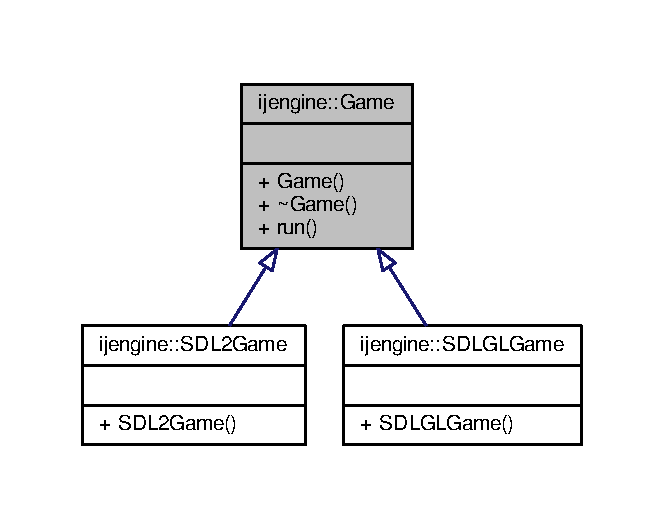
\includegraphics[width=319pt]{classijengine_1_1Game__inherit__graph}
\end{center}
\end{figure}


Collaboration diagram for ijengine\-:\-:Game\-:\nopagebreak
\begin{figure}[H]
\begin{center}
\leavevmode
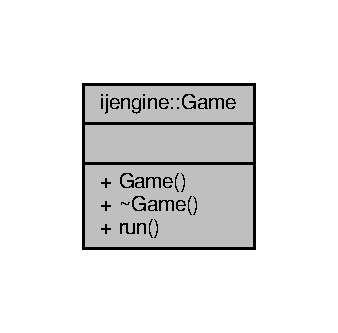
\includegraphics[width=162pt]{classijengine_1_1Game__coll__graph}
\end{center}
\end{figure}
\subsection*{Public Member Functions}
\begin{DoxyCompactItemize}
\item 
\hyperlink{classijengine_1_1Game_a0f299591316c54af58da366f6b7a2795}{Game} ()
\item 
virtual \hyperlink{classijengine_1_1Game_a6f5da74410e764ac27a45224b306a920}{$\sim$\-Game} ()
\item 
int \hyperlink{classijengine_1_1Game_a1a86bc39a6e4c1c5c35f998bc3e969c0}{run} ()
\end{DoxyCompactItemize}


\subsection{Constructor \& Destructor Documentation}
\hypertarget{classijengine_1_1Game_a0f299591316c54af58da366f6b7a2795}{\index{ijengine\-::\-Game@{ijengine\-::\-Game}!Game@{Game}}
\index{Game@{Game}!ijengine::Game@{ijengine\-::\-Game}}
\subsubsection[{Game}]{\setlength{\rightskip}{0pt plus 5cm}ijengine\-::\-Game\-::\-Game (
\begin{DoxyParamCaption}
{}
\end{DoxyParamCaption}
)}}\label{classijengine_1_1Game_a0f299591316c54af58da366f6b7a2795}
\hypertarget{classijengine_1_1Game_a6f5da74410e764ac27a45224b306a920}{\index{ijengine\-::\-Game@{ijengine\-::\-Game}!$\sim$\-Game@{$\sim$\-Game}}
\index{$\sim$\-Game@{$\sim$\-Game}!ijengine::Game@{ijengine\-::\-Game}}
\subsubsection[{$\sim$\-Game}]{\setlength{\rightskip}{0pt plus 5cm}ijengine\-::\-Game\-::$\sim$\-Game (
\begin{DoxyParamCaption}
{}
\end{DoxyParamCaption}
)\hspace{0.3cm}{\ttfamily [virtual]}}}\label{classijengine_1_1Game_a6f5da74410e764ac27a45224b306a920}


\subsection{Member Function Documentation}
\hypertarget{classijengine_1_1Game_a1a86bc39a6e4c1c5c35f998bc3e969c0}{\index{ijengine\-::\-Game@{ijengine\-::\-Game}!run@{run}}
\index{run@{run}!ijengine::Game@{ijengine\-::\-Game}}
\subsubsection[{run}]{\setlength{\rightskip}{0pt plus 5cm}int ijengine\-::\-Game\-::run (
\begin{DoxyParamCaption}
{}
\end{DoxyParamCaption}
)}}\label{classijengine_1_1Game_a1a86bc39a6e4c1c5c35f998bc3e969c0}


The documentation for this class was generated from the following files\-:\begin{DoxyCompactItemize}
\item 
/home/carla/git/ijengine-\/\-I\-C\-G\-\_\-\-G\-L/include/\hyperlink{game_8h}{game.\-h}\item 
/home/carla/git/ijengine-\/\-I\-C\-G\-\_\-\-G\-L/src/\hyperlink{game_8cpp}{game.\-cpp}\end{DoxyCompactItemize}

\hypertarget{classijengine_1_1GameModels}{\section{ijengine\-:\-:Game\-Models Class Reference}
\label{classijengine_1_1GameModels}\index{ijengine\-::\-Game\-Models@{ijengine\-::\-Game\-Models}}
}


{\ttfamily \#include $<$gamemodels.\-h$>$}



Collaboration diagram for ijengine\-:\-:Game\-Models\-:\nopagebreak
\begin{figure}[H]
\begin{center}
\leavevmode
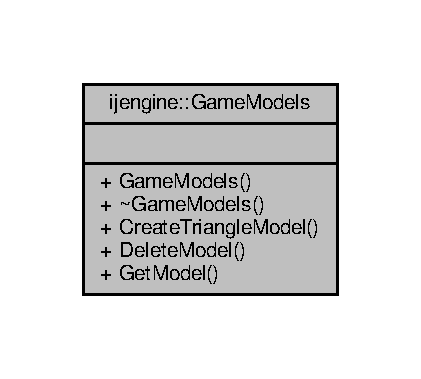
\includegraphics[width=202pt]{classijengine_1_1GameModels__coll__graph}
\end{center}
\end{figure}
\subsection*{Public Member Functions}
\begin{DoxyCompactItemize}
\item 
\hyperlink{classijengine_1_1GameModels_afe97cd039ac920bf467fe803fafd4808}{Game\-Models} ()
\item 
\hyperlink{classijengine_1_1GameModels_ab71ca79d237aa3ace876a1e0ee2250e5}{$\sim$\-Game\-Models} ()
\item 
virtual \hyperlink{classijengine_1_1GameModels_a23361e2d38ee8e35211e6298fd586ce2}{Create\-Triangle\-Model} (const string \&game\-Model\-Name)
\item 
virtual \hyperlink{classijengine_1_1GameModels_ae7a617bd2183603b61e0014aab9ff97a}{Delete\-Model} (const string \&game\-Model\-Name)
\item 
unsigned int \hyperlink{classijengine_1_1GameModels_ad517639f989d88b5cd36fc51319ec336}{Get\-Model} (const string \&game\-Model\-Name)
\end{DoxyCompactItemize}


\subsection{Constructor \& Destructor Documentation}
\hypertarget{classijengine_1_1GameModels_afe97cd039ac920bf467fe803fafd4808}{\index{ijengine\-::\-Game\-Models@{ijengine\-::\-Game\-Models}!Game\-Models@{Game\-Models}}
\index{Game\-Models@{Game\-Models}!ijengine::GameModels@{ijengine\-::\-Game\-Models}}
\subsubsection[{Game\-Models}]{\setlength{\rightskip}{0pt plus 5cm}ijengine\-::\-Game\-Models\-::\-Game\-Models (
\begin{DoxyParamCaption}
{}
\end{DoxyParamCaption}
)}}\label{classijengine_1_1GameModels_afe97cd039ac920bf467fe803fafd4808}
\hypertarget{classijengine_1_1GameModels_ab71ca79d237aa3ace876a1e0ee2250e5}{\index{ijengine\-::\-Game\-Models@{ijengine\-::\-Game\-Models}!$\sim$\-Game\-Models@{$\sim$\-Game\-Models}}
\index{$\sim$\-Game\-Models@{$\sim$\-Game\-Models}!ijengine::GameModels@{ijengine\-::\-Game\-Models}}
\subsubsection[{$\sim$\-Game\-Models}]{\setlength{\rightskip}{0pt plus 5cm}ijengine\-::\-Game\-Models\-::$\sim$\-Game\-Models (
\begin{DoxyParamCaption}
{}
\end{DoxyParamCaption}
)}}\label{classijengine_1_1GameModels_ab71ca79d237aa3ace876a1e0ee2250e5}


\subsection{Member Function Documentation}
\hypertarget{classijengine_1_1GameModels_a23361e2d38ee8e35211e6298fd586ce2}{\index{ijengine\-::\-Game\-Models@{ijengine\-::\-Game\-Models}!Create\-Triangle\-Model@{Create\-Triangle\-Model}}
\index{Create\-Triangle\-Model@{Create\-Triangle\-Model}!ijengine::GameModels@{ijengine\-::\-Game\-Models}}
\subsubsection[{Create\-Triangle\-Model}]{\setlength{\rightskip}{0pt plus 5cm}virtual ijengine\-::\-Game\-Models\-::\-Create\-Triangle\-Model (
\begin{DoxyParamCaption}
\item[{const string \&}]{game\-Model\-Name}
\end{DoxyParamCaption}
)\hspace{0.3cm}{\ttfamily [virtual]}}}\label{classijengine_1_1GameModels_a23361e2d38ee8e35211e6298fd586ce2}
\hypertarget{classijengine_1_1GameModels_ae7a617bd2183603b61e0014aab9ff97a}{\index{ijengine\-::\-Game\-Models@{ijengine\-::\-Game\-Models}!Delete\-Model@{Delete\-Model}}
\index{Delete\-Model@{Delete\-Model}!ijengine::GameModels@{ijengine\-::\-Game\-Models}}
\subsubsection[{Delete\-Model}]{\setlength{\rightskip}{0pt plus 5cm}virtual ijengine\-::\-Game\-Models\-::\-Delete\-Model (
\begin{DoxyParamCaption}
\item[{const string \&}]{game\-Model\-Name}
\end{DoxyParamCaption}
)\hspace{0.3cm}{\ttfamily [virtual]}}}\label{classijengine_1_1GameModels_ae7a617bd2183603b61e0014aab9ff97a}
\hypertarget{classijengine_1_1GameModels_ad517639f989d88b5cd36fc51319ec336}{\index{ijengine\-::\-Game\-Models@{ijengine\-::\-Game\-Models}!Get\-Model@{Get\-Model}}
\index{Get\-Model@{Get\-Model}!ijengine::GameModels@{ijengine\-::\-Game\-Models}}
\subsubsection[{Get\-Model}]{\setlength{\rightskip}{0pt plus 5cm}unsigned int ijengine\-::\-Game\-Models\-::\-Get\-Model (
\begin{DoxyParamCaption}
\item[{const string \&}]{game\-Model\-Name}
\end{DoxyParamCaption}
)}}\label{classijengine_1_1GameModels_ad517639f989d88b5cd36fc51319ec336}


The documentation for this class was generated from the following file\-:\begin{DoxyCompactItemize}
\item 
/home/carla/git/ijengine-\/\-I\-C\-G\-\_\-\-G\-L/include/\hyperlink{gamemodels_8h}{gamemodels.\-h}\end{DoxyCompactItemize}

\hypertarget{classGLrenderer3d}{\section{G\-Lrenderer3d Class Reference}
\label{classGLrenderer3d}\index{G\-Lrenderer3d@{G\-Lrenderer3d}}
}


{\ttfamily \#include $<$glrenderer3d.\-h$>$}



Inheritance diagram for G\-Lrenderer3d\-:\nopagebreak
\begin{figure}[H]
\begin{center}
\leavevmode
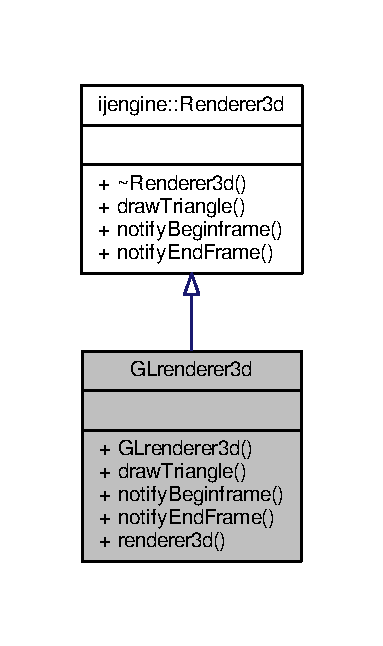
\includegraphics[width=184pt]{classGLrenderer3d__inherit__graph}
\end{center}
\end{figure}


Collaboration diagram for G\-Lrenderer3d\-:\nopagebreak
\begin{figure}[H]
\begin{center}
\leavevmode
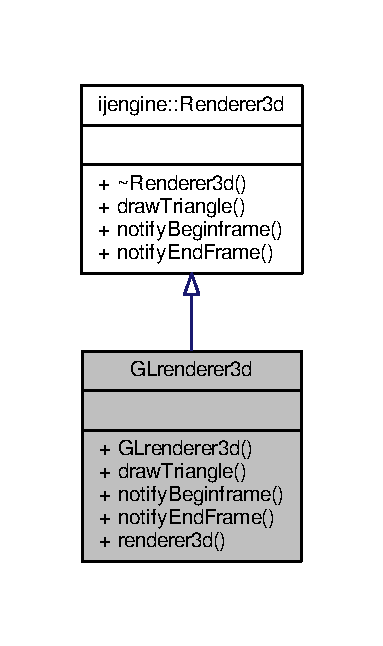
\includegraphics[width=184pt]{classGLrenderer3d__coll__graph}
\end{center}
\end{figure}
\subsection*{Public Member Functions}
\begin{DoxyCompactItemize}
\item 
\hyperlink{classGLrenderer3d_a7cdc3e8f4b5c7fc516e244ace28c26ae}{G\-Lrenderer3d} (S\-D\-L\-\_\-\-Window $\ast$\hyperlink{classGLrenderer3d_a2392453b4b81dd64811898a452042e8d}{renderer3d})
\item 
void \hyperlink{classGLrenderer3d_af10dc480fc22622db6a83c87bb119ca7}{draw\-Triangle} (float x, float y, float z, float scale, int r, int g, int b)
\item 
void \hyperlink{classGLrenderer3d_a69cfa7ad8eac36b068b8cc8e461d7c33}{notify\-Beginframe} ()
\item 
void \hyperlink{classGLrenderer3d_a1625b7fa82863e7f54ba86d2ebe5f7af}{notify\-End\-Frame} ()
\item 
S\-D\-L\-\_\-\-Window $\ast$ \hyperlink{classGLrenderer3d_a2392453b4b81dd64811898a452042e8d}{renderer3d} () const 
\end{DoxyCompactItemize}


\subsection{Constructor \& Destructor Documentation}
\hypertarget{classGLrenderer3d_a7cdc3e8f4b5c7fc516e244ace28c26ae}{\index{G\-Lrenderer3d@{G\-Lrenderer3d}!G\-Lrenderer3d@{G\-Lrenderer3d}}
\index{G\-Lrenderer3d@{G\-Lrenderer3d}!GLrenderer3d@{G\-Lrenderer3d}}
\subsubsection[{G\-Lrenderer3d}]{\setlength{\rightskip}{0pt plus 5cm}G\-Lrenderer3d\-::\-G\-Lrenderer3d (
\begin{DoxyParamCaption}
\item[{S\-D\-L\-\_\-\-Window $\ast$}]{renderer3d}
\end{DoxyParamCaption}
)}}\label{classGLrenderer3d_a7cdc3e8f4b5c7fc516e244ace28c26ae}


\subsection{Member Function Documentation}
\hypertarget{classGLrenderer3d_af10dc480fc22622db6a83c87bb119ca7}{\index{G\-Lrenderer3d@{G\-Lrenderer3d}!draw\-Triangle@{draw\-Triangle}}
\index{draw\-Triangle@{draw\-Triangle}!GLrenderer3d@{G\-Lrenderer3d}}
\subsubsection[{draw\-Triangle}]{\setlength{\rightskip}{0pt plus 5cm}void G\-Lrenderer3d\-::draw\-Triangle (
\begin{DoxyParamCaption}
\item[{float}]{x, }
\item[{float}]{y, }
\item[{float}]{z, }
\item[{float}]{scale, }
\item[{int}]{r, }
\item[{int}]{g, }
\item[{int}]{b}
\end{DoxyParamCaption}
)\hspace{0.3cm}{\ttfamily [virtual]}}}\label{classGLrenderer3d_af10dc480fc22622db6a83c87bb119ca7}


Implements \hyperlink{classijengine_1_1Renderer3d_a105c5b22d90584aeda18cafdd15650da}{ijengine\-::\-Renderer3d}.

\hypertarget{classGLrenderer3d_a69cfa7ad8eac36b068b8cc8e461d7c33}{\index{G\-Lrenderer3d@{G\-Lrenderer3d}!notify\-Beginframe@{notify\-Beginframe}}
\index{notify\-Beginframe@{notify\-Beginframe}!GLrenderer3d@{G\-Lrenderer3d}}
\subsubsection[{notify\-Beginframe}]{\setlength{\rightskip}{0pt plus 5cm}void G\-Lrenderer3d\-::notify\-Beginframe (
\begin{DoxyParamCaption}
{}
\end{DoxyParamCaption}
)\hspace{0.3cm}{\ttfamily [virtual]}}}\label{classGLrenderer3d_a69cfa7ad8eac36b068b8cc8e461d7c33}


Implements \hyperlink{classijengine_1_1Renderer3d_a4f2d16d72f210445fdb9210b3fce33bf}{ijengine\-::\-Renderer3d}.

\hypertarget{classGLrenderer3d_a1625b7fa82863e7f54ba86d2ebe5f7af}{\index{G\-Lrenderer3d@{G\-Lrenderer3d}!notify\-End\-Frame@{notify\-End\-Frame}}
\index{notify\-End\-Frame@{notify\-End\-Frame}!GLrenderer3d@{G\-Lrenderer3d}}
\subsubsection[{notify\-End\-Frame}]{\setlength{\rightskip}{0pt plus 5cm}void G\-Lrenderer3d\-::notify\-End\-Frame (
\begin{DoxyParamCaption}
{}
\end{DoxyParamCaption}
)\hspace{0.3cm}{\ttfamily [virtual]}}}\label{classGLrenderer3d_a1625b7fa82863e7f54ba86d2ebe5f7af}


Implements \hyperlink{classijengine_1_1Renderer3d_af0a21ea9fc5ebd8e30922047bf743a14}{ijengine\-::\-Renderer3d}.

\hypertarget{classGLrenderer3d_a2392453b4b81dd64811898a452042e8d}{\index{G\-Lrenderer3d@{G\-Lrenderer3d}!renderer3d@{renderer3d}}
\index{renderer3d@{renderer3d}!GLrenderer3d@{G\-Lrenderer3d}}
\subsubsection[{renderer3d}]{\setlength{\rightskip}{0pt plus 5cm}S\-D\-L\-\_\-\-Window $\ast$ G\-Lrenderer3d\-::renderer3d (
\begin{DoxyParamCaption}
{}
\end{DoxyParamCaption}
) const}}\label{classGLrenderer3d_a2392453b4b81dd64811898a452042e8d}


The documentation for this class was generated from the following files\-:\begin{DoxyCompactItemize}
\item 
/home/carla/git/ijengine-\/\-I\-C\-G\-\_\-\-G\-L/include/\hyperlink{glrenderer3d_8h}{glrenderer3d.\-h}\item 
/home/carla/git/ijengine-\/\-I\-C\-G\-\_\-\-G\-L/src/\hyperlink{glrenderer3d_8cpp}{glrenderer3d.\-cpp}\end{DoxyCompactItemize}

\hypertarget{classijengine_1_1Lib}{\section{ijengine\-:\-:Lib Class Reference}
\label{classijengine_1_1Lib}\index{ijengine\-::\-Lib@{ijengine\-::\-Lib}}
}


{\ttfamily \#include $<$libs.\-h$>$}



Inheritance diagram for ijengine\-:\-:Lib\-:\nopagebreak
\begin{figure}[H]
\begin{center}
\leavevmode
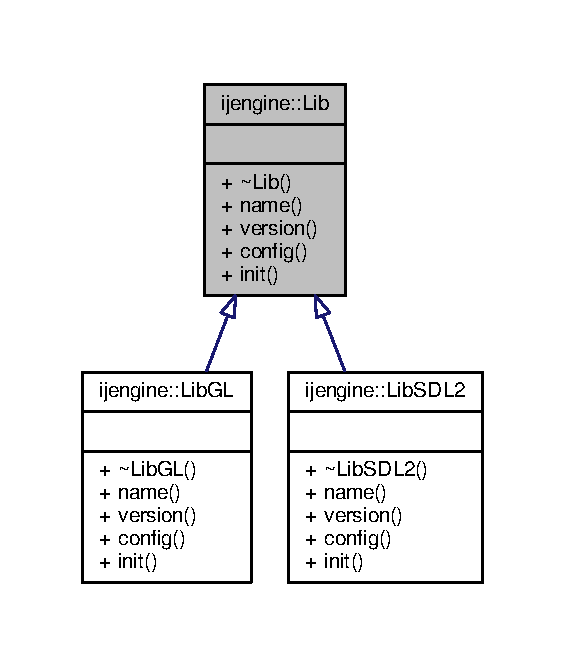
\includegraphics[width=271pt]{classijengine_1_1Lib__inherit__graph}
\end{center}
\end{figure}


Collaboration diagram for ijengine\-:\-:Lib\-:\nopagebreak
\begin{figure}[H]
\begin{center}
\leavevmode
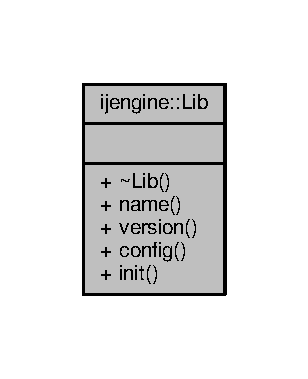
\includegraphics[width=148pt]{classijengine_1_1Lib__coll__graph}
\end{center}
\end{figure}
\subsection*{Public Member Functions}
\begin{DoxyCompactItemize}
\item 
virtual \hyperlink{classijengine_1_1Lib_a04fe6731bd47a82928f19b71fc611c7a}{$\sim$\-Lib} ()=default
\item 
virtual string \hyperlink{classijengine_1_1Lib_a4b9c9bf0de12262823bf9f9543b7c24e}{name} () const =0
\item 
virtual string \hyperlink{classijengine_1_1Lib_a0fdaa7786c6bd7afaab1be8d58224630}{version} () const =0
\item 
virtual void \hyperlink{classijengine_1_1Lib_a669f2c5e4bcb92d144feab5d25f1610f}{config} (const string \&param, const string \&value)=0
\item 
virtual void \hyperlink{classijengine_1_1Lib_a06cbf2575cf46251daa384d94ccf9e4f}{init} ()=0
\end{DoxyCompactItemize}


\subsection{Constructor \& Destructor Documentation}
\hypertarget{classijengine_1_1Lib_a04fe6731bd47a82928f19b71fc611c7a}{\index{ijengine\-::\-Lib@{ijengine\-::\-Lib}!$\sim$\-Lib@{$\sim$\-Lib}}
\index{$\sim$\-Lib@{$\sim$\-Lib}!ijengine::Lib@{ijengine\-::\-Lib}}
\subsubsection[{$\sim$\-Lib}]{\setlength{\rightskip}{0pt plus 5cm}virtual ijengine\-::\-Lib\-::$\sim$\-Lib (
\begin{DoxyParamCaption}
{}
\end{DoxyParamCaption}
)\hspace{0.3cm}{\ttfamily [virtual]}, {\ttfamily [default]}}}\label{classijengine_1_1Lib_a04fe6731bd47a82928f19b71fc611c7a}


\subsection{Member Function Documentation}
\hypertarget{classijengine_1_1Lib_a669f2c5e4bcb92d144feab5d25f1610f}{\index{ijengine\-::\-Lib@{ijengine\-::\-Lib}!config@{config}}
\index{config@{config}!ijengine::Lib@{ijengine\-::\-Lib}}
\subsubsection[{config}]{\setlength{\rightskip}{0pt plus 5cm}virtual void ijengine\-::\-Lib\-::config (
\begin{DoxyParamCaption}
\item[{const string \&}]{param, }
\item[{const string \&}]{value}
\end{DoxyParamCaption}
)\hspace{0.3cm}{\ttfamily [pure virtual]}}}\label{classijengine_1_1Lib_a669f2c5e4bcb92d144feab5d25f1610f}


Implemented in \hyperlink{classijengine_1_1LibGL_a7b8128296f4f1aacefb608468baa531a}{ijengine\-::\-Lib\-G\-L}, and \hyperlink{classijengine_1_1LibSDL2_a52dcf9c6061a1f0c917e2c4762491f18}{ijengine\-::\-Lib\-S\-D\-L2}.

\hypertarget{classijengine_1_1Lib_a06cbf2575cf46251daa384d94ccf9e4f}{\index{ijengine\-::\-Lib@{ijengine\-::\-Lib}!init@{init}}
\index{init@{init}!ijengine::Lib@{ijengine\-::\-Lib}}
\subsubsection[{init}]{\setlength{\rightskip}{0pt plus 5cm}virtual void ijengine\-::\-Lib\-::init (
\begin{DoxyParamCaption}
{}
\end{DoxyParamCaption}
)\hspace{0.3cm}{\ttfamily [pure virtual]}}}\label{classijengine_1_1Lib_a06cbf2575cf46251daa384d94ccf9e4f}


Implemented in \hyperlink{classijengine_1_1LibGL_a46f71fb7c9ecce992ecb5fc0a1122b41}{ijengine\-::\-Lib\-G\-L}, and \hyperlink{classijengine_1_1LibSDL2_a473340c2f65b610b884a473813fd0b33}{ijengine\-::\-Lib\-S\-D\-L2}.

\hypertarget{classijengine_1_1Lib_a4b9c9bf0de12262823bf9f9543b7c24e}{\index{ijengine\-::\-Lib@{ijengine\-::\-Lib}!name@{name}}
\index{name@{name}!ijengine::Lib@{ijengine\-::\-Lib}}
\subsubsection[{name}]{\setlength{\rightskip}{0pt plus 5cm}virtual string ijengine\-::\-Lib\-::name (
\begin{DoxyParamCaption}
{}
\end{DoxyParamCaption}
) const\hspace{0.3cm}{\ttfamily [pure virtual]}}}\label{classijengine_1_1Lib_a4b9c9bf0de12262823bf9f9543b7c24e}


Implemented in \hyperlink{classijengine_1_1LibGL_afe0784e342131c99f3db81a1c10dbd55}{ijengine\-::\-Lib\-G\-L}, and \hyperlink{classijengine_1_1LibSDL2_ad2b1d60f874de08cf14f4b0b529f7ad2}{ijengine\-::\-Lib\-S\-D\-L2}.

\hypertarget{classijengine_1_1Lib_a0fdaa7786c6bd7afaab1be8d58224630}{\index{ijengine\-::\-Lib@{ijengine\-::\-Lib}!version@{version}}
\index{version@{version}!ijengine::Lib@{ijengine\-::\-Lib}}
\subsubsection[{version}]{\setlength{\rightskip}{0pt plus 5cm}virtual string ijengine\-::\-Lib\-::version (
\begin{DoxyParamCaption}
{}
\end{DoxyParamCaption}
) const\hspace{0.3cm}{\ttfamily [pure virtual]}}}\label{classijengine_1_1Lib_a0fdaa7786c6bd7afaab1be8d58224630}


Implemented in \hyperlink{classijengine_1_1LibGL_abf2adaac930d5e0d036c65e30f718dc3}{ijengine\-::\-Lib\-G\-L}, and \hyperlink{classijengine_1_1LibSDL2_a79988e10ed910e3c760d137209fb107f}{ijengine\-::\-Lib\-S\-D\-L2}.



The documentation for this class was generated from the following file\-:\begin{DoxyCompactItemize}
\item 
/home/carla/git/ijengine-\/\-I\-C\-G\-\_\-\-G\-L/include/\hyperlink{libs_8h}{libs.\-h}\end{DoxyCompactItemize}

\hypertarget{classijengine_1_1LibGL}{\section{ijengine\-:\-:Lib\-G\-L Class Reference}
\label{classijengine_1_1LibGL}\index{ijengine\-::\-Lib\-G\-L@{ijengine\-::\-Lib\-G\-L}}
}


{\ttfamily \#include $<$libgl.\-h$>$}



Inheritance diagram for ijengine\-:\-:Lib\-G\-L\-:\nopagebreak
\begin{figure}[H]
\begin{center}
\leavevmode
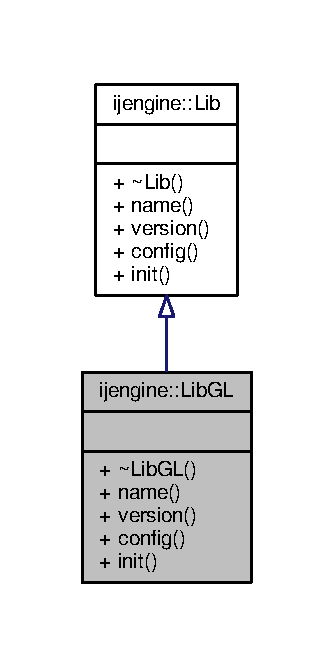
\includegraphics[width=160pt]{classijengine_1_1LibGL__inherit__graph}
\end{center}
\end{figure}


Collaboration diagram for ijengine\-:\-:Lib\-G\-L\-:\nopagebreak
\begin{figure}[H]
\begin{center}
\leavevmode
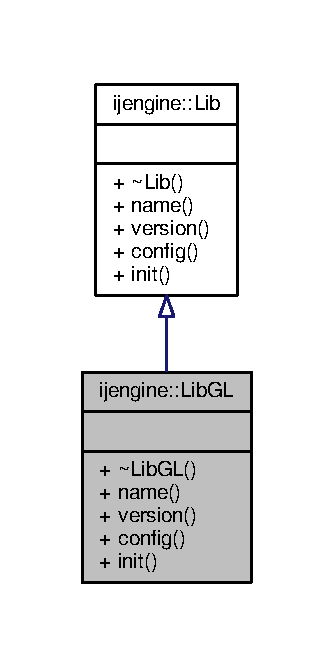
\includegraphics[width=160pt]{classijengine_1_1LibGL__coll__graph}
\end{center}
\end{figure}
\subsection*{Public Member Functions}
\begin{DoxyCompactItemize}
\item 
\hyperlink{classijengine_1_1LibGL_a37b2bb569fe108f2b03aa1987be3917d}{$\sim$\-Lib\-G\-L} ()
\item 
string \hyperlink{classijengine_1_1LibGL_afe0784e342131c99f3db81a1c10dbd55}{name} () const 
\item 
string \hyperlink{classijengine_1_1LibGL_abf2adaac930d5e0d036c65e30f718dc3}{version} () const 
\item 
void \hyperlink{classijengine_1_1LibGL_a7b8128296f4f1aacefb608468baa531a}{config} (const string \&param, const string \&value)
\item 
void \hyperlink{classijengine_1_1LibGL_a46f71fb7c9ecce992ecb5fc0a1122b41}{init} ()
\end{DoxyCompactItemize}


\subsection{Constructor \& Destructor Documentation}
\hypertarget{classijengine_1_1LibGL_a37b2bb569fe108f2b03aa1987be3917d}{\index{ijengine\-::\-Lib\-G\-L@{ijengine\-::\-Lib\-G\-L}!$\sim$\-Lib\-G\-L@{$\sim$\-Lib\-G\-L}}
\index{$\sim$\-Lib\-G\-L@{$\sim$\-Lib\-G\-L}!ijengine::LibGL@{ijengine\-::\-Lib\-G\-L}}
\subsubsection[{$\sim$\-Lib\-G\-L}]{\setlength{\rightskip}{0pt plus 5cm}ijengine\-::\-Lib\-G\-L\-::$\sim$\-Lib\-G\-L (
\begin{DoxyParamCaption}
{}
\end{DoxyParamCaption}
)}}\label{classijengine_1_1LibGL_a37b2bb569fe108f2b03aa1987be3917d}


\subsection{Member Function Documentation}
\hypertarget{classijengine_1_1LibGL_a7b8128296f4f1aacefb608468baa531a}{\index{ijengine\-::\-Lib\-G\-L@{ijengine\-::\-Lib\-G\-L}!config@{config}}
\index{config@{config}!ijengine::LibGL@{ijengine\-::\-Lib\-G\-L}}
\subsubsection[{config}]{\setlength{\rightskip}{0pt plus 5cm}void ijengine\-::\-Lib\-G\-L\-::config (
\begin{DoxyParamCaption}
\item[{const string \&}]{param, }
\item[{const string \&}]{value}
\end{DoxyParamCaption}
)\hspace{0.3cm}{\ttfamily [virtual]}}}\label{classijengine_1_1LibGL_a7b8128296f4f1aacefb608468baa531a}


Implements \hyperlink{classijengine_1_1Lib_a669f2c5e4bcb92d144feab5d25f1610f}{ijengine\-::\-Lib}.

\hypertarget{classijengine_1_1LibGL_a46f71fb7c9ecce992ecb5fc0a1122b41}{\index{ijengine\-::\-Lib\-G\-L@{ijengine\-::\-Lib\-G\-L}!init@{init}}
\index{init@{init}!ijengine::LibGL@{ijengine\-::\-Lib\-G\-L}}
\subsubsection[{init}]{\setlength{\rightskip}{0pt plus 5cm}void ijengine\-::\-Lib\-G\-L\-::init (
\begin{DoxyParamCaption}
{}
\end{DoxyParamCaption}
)\hspace{0.3cm}{\ttfamily [virtual]}}}\label{classijengine_1_1LibGL_a46f71fb7c9ecce992ecb5fc0a1122b41}


Implements \hyperlink{classijengine_1_1Lib_a06cbf2575cf46251daa384d94ccf9e4f}{ijengine\-::\-Lib}.

\hypertarget{classijengine_1_1LibGL_afe0784e342131c99f3db81a1c10dbd55}{\index{ijengine\-::\-Lib\-G\-L@{ijengine\-::\-Lib\-G\-L}!name@{name}}
\index{name@{name}!ijengine::LibGL@{ijengine\-::\-Lib\-G\-L}}
\subsubsection[{name}]{\setlength{\rightskip}{0pt plus 5cm}string ijengine\-::\-Lib\-G\-L\-::name (
\begin{DoxyParamCaption}
{}
\end{DoxyParamCaption}
) const\hspace{0.3cm}{\ttfamily [virtual]}}}\label{classijengine_1_1LibGL_afe0784e342131c99f3db81a1c10dbd55}


Implements \hyperlink{classijengine_1_1Lib_a4b9c9bf0de12262823bf9f9543b7c24e}{ijengine\-::\-Lib}.

\hypertarget{classijengine_1_1LibGL_abf2adaac930d5e0d036c65e30f718dc3}{\index{ijengine\-::\-Lib\-G\-L@{ijengine\-::\-Lib\-G\-L}!version@{version}}
\index{version@{version}!ijengine::LibGL@{ijengine\-::\-Lib\-G\-L}}
\subsubsection[{version}]{\setlength{\rightskip}{0pt plus 5cm}string ijengine\-::\-Lib\-G\-L\-::version (
\begin{DoxyParamCaption}
{}
\end{DoxyParamCaption}
) const\hspace{0.3cm}{\ttfamily [virtual]}}}\label{classijengine_1_1LibGL_abf2adaac930d5e0d036c65e30f718dc3}


Implements \hyperlink{classijengine_1_1Lib_a0fdaa7786c6bd7afaab1be8d58224630}{ijengine\-::\-Lib}.



The documentation for this class was generated from the following files\-:\begin{DoxyCompactItemize}
\item 
/home/carla/git/ijengine-\/\-I\-C\-G\-\_\-\-G\-L/include/\hyperlink{libgl_8h}{libgl.\-h}\item 
/home/carla/git/ijengine-\/\-I\-C\-G\-\_\-\-G\-L/src/\hyperlink{libgl_8cpp}{libgl.\-cpp}\end{DoxyCompactItemize}

\hypertarget{classijengine_1_1LibSDL2}{\section{ijengine\-:\-:Lib\-S\-D\-L2 Class Reference}
\label{classijengine_1_1LibSDL2}\index{ijengine\-::\-Lib\-S\-D\-L2@{ijengine\-::\-Lib\-S\-D\-L2}}
}


{\ttfamily \#include $<$sdl2.\-h$>$}



Inheritance diagram for ijengine\-:\-:Lib\-S\-D\-L2\-:\nopagebreak
\begin{figure}[H]
\begin{center}
\leavevmode
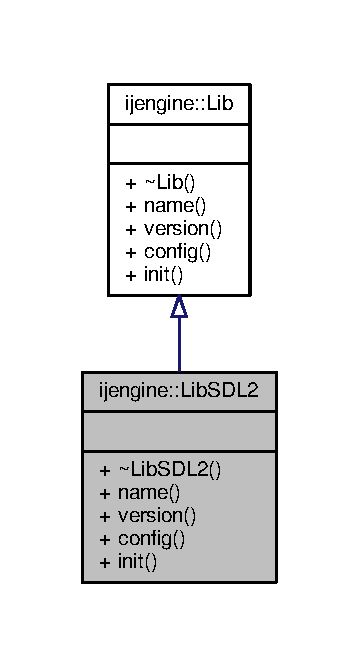
\includegraphics[width=172pt]{classijengine_1_1LibSDL2__inherit__graph}
\end{center}
\end{figure}


Collaboration diagram for ijengine\-:\-:Lib\-S\-D\-L2\-:\nopagebreak
\begin{figure}[H]
\begin{center}
\leavevmode
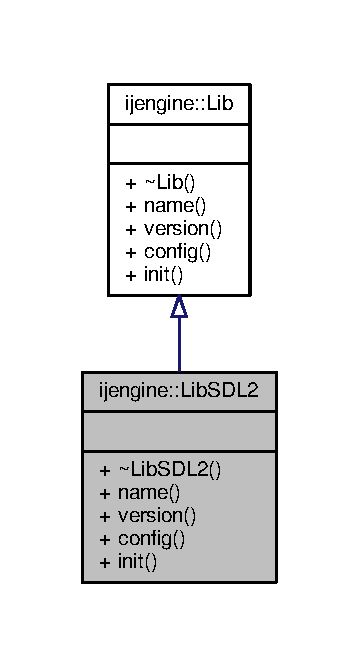
\includegraphics[width=172pt]{classijengine_1_1LibSDL2__coll__graph}
\end{center}
\end{figure}
\subsection*{Public Member Functions}
\begin{DoxyCompactItemize}
\item 
\hyperlink{classijengine_1_1LibSDL2_abd520997dff6073b13d22f35751127b4}{$\sim$\-Lib\-S\-D\-L2} ()
\item 
string \hyperlink{classijengine_1_1LibSDL2_ad2b1d60f874de08cf14f4b0b529f7ad2}{name} () const 
\item 
string \hyperlink{classijengine_1_1LibSDL2_a79988e10ed910e3c760d137209fb107f}{version} () const 
\item 
void \hyperlink{classijengine_1_1LibSDL2_a52dcf9c6061a1f0c917e2c4762491f18}{config} (const string \&param, const string \&value)
\item 
void \hyperlink{classijengine_1_1LibSDL2_a473340c2f65b610b884a473813fd0b33}{init} ()
\end{DoxyCompactItemize}


\subsection{Constructor \& Destructor Documentation}
\hypertarget{classijengine_1_1LibSDL2_abd520997dff6073b13d22f35751127b4}{\index{ijengine\-::\-Lib\-S\-D\-L2@{ijengine\-::\-Lib\-S\-D\-L2}!$\sim$\-Lib\-S\-D\-L2@{$\sim$\-Lib\-S\-D\-L2}}
\index{$\sim$\-Lib\-S\-D\-L2@{$\sim$\-Lib\-S\-D\-L2}!ijengine::LibSDL2@{ijengine\-::\-Lib\-S\-D\-L2}}
\subsubsection[{$\sim$\-Lib\-S\-D\-L2}]{\setlength{\rightskip}{0pt plus 5cm}ijengine\-::\-Lib\-S\-D\-L2\-::$\sim$\-Lib\-S\-D\-L2 (
\begin{DoxyParamCaption}
{}
\end{DoxyParamCaption}
)}}\label{classijengine_1_1LibSDL2_abd520997dff6073b13d22f35751127b4}


\subsection{Member Function Documentation}
\hypertarget{classijengine_1_1LibSDL2_a52dcf9c6061a1f0c917e2c4762491f18}{\index{ijengine\-::\-Lib\-S\-D\-L2@{ijengine\-::\-Lib\-S\-D\-L2}!config@{config}}
\index{config@{config}!ijengine::LibSDL2@{ijengine\-::\-Lib\-S\-D\-L2}}
\subsubsection[{config}]{\setlength{\rightskip}{0pt plus 5cm}void ijengine\-::\-Lib\-S\-D\-L2\-::config (
\begin{DoxyParamCaption}
\item[{const string \&}]{param, }
\item[{const string \&}]{value}
\end{DoxyParamCaption}
)\hspace{0.3cm}{\ttfamily [virtual]}}}\label{classijengine_1_1LibSDL2_a52dcf9c6061a1f0c917e2c4762491f18}


Implements \hyperlink{classijengine_1_1Lib_a669f2c5e4bcb92d144feab5d25f1610f}{ijengine\-::\-Lib}.

\hypertarget{classijengine_1_1LibSDL2_a473340c2f65b610b884a473813fd0b33}{\index{ijengine\-::\-Lib\-S\-D\-L2@{ijengine\-::\-Lib\-S\-D\-L2}!init@{init}}
\index{init@{init}!ijengine::LibSDL2@{ijengine\-::\-Lib\-S\-D\-L2}}
\subsubsection[{init}]{\setlength{\rightskip}{0pt plus 5cm}void ijengine\-::\-Lib\-S\-D\-L2\-::init (
\begin{DoxyParamCaption}
{}
\end{DoxyParamCaption}
)\hspace{0.3cm}{\ttfamily [virtual]}}}\label{classijengine_1_1LibSDL2_a473340c2f65b610b884a473813fd0b33}


Implements \hyperlink{classijengine_1_1Lib_a06cbf2575cf46251daa384d94ccf9e4f}{ijengine\-::\-Lib}.

\hypertarget{classijengine_1_1LibSDL2_ad2b1d60f874de08cf14f4b0b529f7ad2}{\index{ijengine\-::\-Lib\-S\-D\-L2@{ijengine\-::\-Lib\-S\-D\-L2}!name@{name}}
\index{name@{name}!ijengine::LibSDL2@{ijengine\-::\-Lib\-S\-D\-L2}}
\subsubsection[{name}]{\setlength{\rightskip}{0pt plus 5cm}string ijengine\-::\-Lib\-S\-D\-L2\-::name (
\begin{DoxyParamCaption}
{}
\end{DoxyParamCaption}
) const\hspace{0.3cm}{\ttfamily [virtual]}}}\label{classijengine_1_1LibSDL2_ad2b1d60f874de08cf14f4b0b529f7ad2}


Implements \hyperlink{classijengine_1_1Lib_a4b9c9bf0de12262823bf9f9543b7c24e}{ijengine\-::\-Lib}.

\hypertarget{classijengine_1_1LibSDL2_a79988e10ed910e3c760d137209fb107f}{\index{ijengine\-::\-Lib\-S\-D\-L2@{ijengine\-::\-Lib\-S\-D\-L2}!version@{version}}
\index{version@{version}!ijengine::LibSDL2@{ijengine\-::\-Lib\-S\-D\-L2}}
\subsubsection[{version}]{\setlength{\rightskip}{0pt plus 5cm}string ijengine\-::\-Lib\-S\-D\-L2\-::version (
\begin{DoxyParamCaption}
{}
\end{DoxyParamCaption}
) const\hspace{0.3cm}{\ttfamily [virtual]}}}\label{classijengine_1_1LibSDL2_a79988e10ed910e3c760d137209fb107f}


Implements \hyperlink{classijengine_1_1Lib_a0fdaa7786c6bd7afaab1be8d58224630}{ijengine\-::\-Lib}.



The documentation for this class was generated from the following files\-:\begin{DoxyCompactItemize}
\item 
/home/carla/git/ijengine-\/\-I\-C\-G\-\_\-\-G\-L/include/\hyperlink{sdl2_8h}{sdl2.\-h}\item 
/home/carla/git/ijengine-\/\-I\-C\-G\-\_\-\-G\-L/src/\hyperlink{sdl2_8cpp}{sdl2.\-cpp}\end{DoxyCompactItemize}

\hypertarget{structijengine_1_1Model}{\section{ijengine\-:\-:Model Class Reference}
\label{structijengine_1_1Model}\index{ijengine\-::\-Model@{ijengine\-::\-Model}}
}


{\ttfamily \#include $<$gamemodels.\-h$>$}



Inheritance diagram for ijengine\-:\-:Model\-:\nopagebreak
\begin{figure}[H]
\begin{center}
\leavevmode
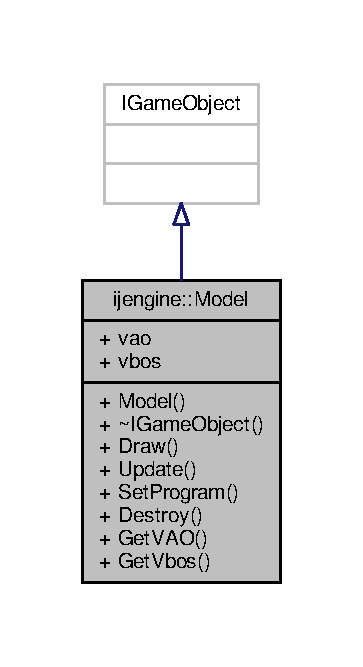
\includegraphics[width=174pt]{structijengine_1_1Model__inherit__graph}
\end{center}
\end{figure}


Collaboration diagram for ijengine\-:\-:Model\-:\nopagebreak
\begin{figure}[H]
\begin{center}
\leavevmode
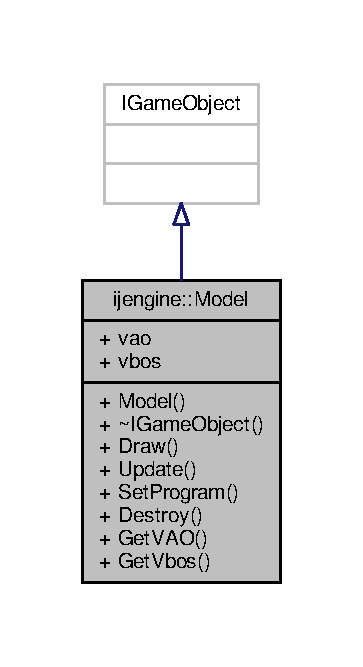
\includegraphics[width=174pt]{structijengine_1_1Model__coll__graph}
\end{center}
\end{figure}
\subsection*{Public Member Functions}
\begin{DoxyCompactItemize}
\item 
\hyperlink{structijengine_1_1Model_a78b86cd4f07879f775615b26a6616df7}{Model} ()
\item 
virtual \hyperlink{structijengine_1_1Model_a47b164e36700e7353da3e4a85ff636c3}{$\sim$\-I\-Game\-Object} ()=0
\item 
virtual void \hyperlink{structijengine_1_1Model_aff9561a2feecc7a232bc1e7ac97475ad}{Draw} ()=0
\item 
virtual \hyperlink{structijengine_1_1Model_a035780f6602643ddb3674ddc9b400aed}{Update} ()=0
\item 
virtual void \hyperlink{structijengine_1_1Model_a85245d758ddabf9dcfcf5f542999ad87}{Set\-Program} (G\-Luint shader\-Name)=0
\item 
virtual void \hyperlink{structijengine_1_1Model_adb632186be89b40c5e9cc5f355fc05e6}{Destroy} ()
\item 
virtual G\-Luint \hyperlink{structijengine_1_1Model_ae95b4198766618c787ee963bb1c75b81}{Get\-V\-A\-O} () const =0
\item 
virtual const vector$<$ G\-Luint $>$ \& \hyperlink{structijengine_1_1Model_a5b560d6f47bd2b0999886751f1fd743e}{Get\-Vbos} () const =0
\end{DoxyCompactItemize}
\subsection*{Public Attributes}
\begin{DoxyCompactItemize}
\item 
unsigned int \hyperlink{structijengine_1_1Model_ac8e3b6e589118cfcc8141855262218bf}{vao}
\item 
vector$<$ unsigned int $>$ \hyperlink{structijengine_1_1Model_a8228166fb6499a5b340981b15b27c098}{vbos}
\end{DoxyCompactItemize}


\subsection{Constructor \& Destructor Documentation}
\hypertarget{structijengine_1_1Model_a78b86cd4f07879f775615b26a6616df7}{\index{ijengine\-::\-Model@{ijengine\-::\-Model}!Model@{Model}}
\index{Model@{Model}!ijengine::Model@{ijengine\-::\-Model}}
\subsubsection[{Model}]{\setlength{\rightskip}{0pt plus 5cm}ijengine\-::\-Model\-::\-Model (
\begin{DoxyParamCaption}
{}
\end{DoxyParamCaption}
)\hspace{0.3cm}{\ttfamily [inline]}}}\label{structijengine_1_1Model_a78b86cd4f07879f775615b26a6616df7}
\hypertarget{structijengine_1_1Model_a47b164e36700e7353da3e4a85ff636c3}{\index{ijengine\-::\-Model@{ijengine\-::\-Model}!$\sim$\-I\-Game\-Object@{$\sim$\-I\-Game\-Object}}
\index{$\sim$\-I\-Game\-Object@{$\sim$\-I\-Game\-Object}!ijengine::Model@{ijengine\-::\-Model}}
\subsubsection[{$\sim$\-I\-Game\-Object}]{\setlength{\rightskip}{0pt plus 5cm}virtual ijengine\-::\-Model\-::$\sim$\-I\-Game\-Object (
\begin{DoxyParamCaption}
{}
\end{DoxyParamCaption}
)\hspace{0.3cm}{\ttfamily [pure virtual]}}}\label{structijengine_1_1Model_a47b164e36700e7353da3e4a85ff636c3}


\subsection{Member Function Documentation}
\hypertarget{structijengine_1_1Model_adb632186be89b40c5e9cc5f355fc05e6}{\index{ijengine\-::\-Model@{ijengine\-::\-Model}!Destroy@{Destroy}}
\index{Destroy@{Destroy}!ijengine::Model@{ijengine\-::\-Model}}
\subsubsection[{Destroy}]{\setlength{\rightskip}{0pt plus 5cm}virtual void ijengine\-::\-Model\-::\-Destroy (
\begin{DoxyParamCaption}
{}
\end{DoxyParamCaption}
)\hspace{0.3cm}{\ttfamily [virtual]}}}\label{structijengine_1_1Model_adb632186be89b40c5e9cc5f355fc05e6}
\hypertarget{structijengine_1_1Model_aff9561a2feecc7a232bc1e7ac97475ad}{\index{ijengine\-::\-Model@{ijengine\-::\-Model}!Draw@{Draw}}
\index{Draw@{Draw}!ijengine::Model@{ijengine\-::\-Model}}
\subsubsection[{Draw}]{\setlength{\rightskip}{0pt plus 5cm}virtual void ijengine\-::\-Model\-::\-Draw (
\begin{DoxyParamCaption}
{}
\end{DoxyParamCaption}
)\hspace{0.3cm}{\ttfamily [pure virtual]}}}\label{structijengine_1_1Model_aff9561a2feecc7a232bc1e7ac97475ad}
\hypertarget{structijengine_1_1Model_ae95b4198766618c787ee963bb1c75b81}{\index{ijengine\-::\-Model@{ijengine\-::\-Model}!Get\-V\-A\-O@{Get\-V\-A\-O}}
\index{Get\-V\-A\-O@{Get\-V\-A\-O}!ijengine::Model@{ijengine\-::\-Model}}
\subsubsection[{Get\-V\-A\-O}]{\setlength{\rightskip}{0pt plus 5cm}virtual G\-Luint ijengine\-::\-Model\-::\-Get\-V\-A\-O (
\begin{DoxyParamCaption}
{}
\end{DoxyParamCaption}
) const\hspace{0.3cm}{\ttfamily [pure virtual]}}}\label{structijengine_1_1Model_ae95b4198766618c787ee963bb1c75b81}
\hypertarget{structijengine_1_1Model_a5b560d6f47bd2b0999886751f1fd743e}{\index{ijengine\-::\-Model@{ijengine\-::\-Model}!Get\-Vbos@{Get\-Vbos}}
\index{Get\-Vbos@{Get\-Vbos}!ijengine::Model@{ijengine\-::\-Model}}
\subsubsection[{Get\-Vbos}]{\setlength{\rightskip}{0pt plus 5cm}virtual const vector$<$G\-Luint$>$\& ijengine\-::\-Model\-::\-Get\-Vbos (
\begin{DoxyParamCaption}
{}
\end{DoxyParamCaption}
) const\hspace{0.3cm}{\ttfamily [pure virtual]}}}\label{structijengine_1_1Model_a5b560d6f47bd2b0999886751f1fd743e}
\hypertarget{structijengine_1_1Model_a85245d758ddabf9dcfcf5f542999ad87}{\index{ijengine\-::\-Model@{ijengine\-::\-Model}!Set\-Program@{Set\-Program}}
\index{Set\-Program@{Set\-Program}!ijengine::Model@{ijengine\-::\-Model}}
\subsubsection[{Set\-Program}]{\setlength{\rightskip}{0pt plus 5cm}virtual void ijengine\-::\-Model\-::\-Set\-Program (
\begin{DoxyParamCaption}
\item[{G\-Luint}]{shader\-Name}
\end{DoxyParamCaption}
)\hspace{0.3cm}{\ttfamily [pure virtual]}}}\label{structijengine_1_1Model_a85245d758ddabf9dcfcf5f542999ad87}
\hypertarget{structijengine_1_1Model_a035780f6602643ddb3674ddc9b400aed}{\index{ijengine\-::\-Model@{ijengine\-::\-Model}!Update@{Update}}
\index{Update@{Update}!ijengine::Model@{ijengine\-::\-Model}}
\subsubsection[{Update}]{\setlength{\rightskip}{0pt plus 5cm}virtual ijengine\-::\-Model\-::\-Update (
\begin{DoxyParamCaption}
{}
\end{DoxyParamCaption}
)\hspace{0.3cm}{\ttfamily [pure virtual]}}}\label{structijengine_1_1Model_a035780f6602643ddb3674ddc9b400aed}


\subsection{Member Data Documentation}
\hypertarget{structijengine_1_1Model_ac8e3b6e589118cfcc8141855262218bf}{\index{ijengine\-::\-Model@{ijengine\-::\-Model}!vao@{vao}}
\index{vao@{vao}!ijengine::Model@{ijengine\-::\-Model}}
\subsubsection[{vao}]{\setlength{\rightskip}{0pt plus 5cm}unsigned int ijengine\-::\-Model\-::vao}}\label{structijengine_1_1Model_ac8e3b6e589118cfcc8141855262218bf}
\hypertarget{structijengine_1_1Model_a8228166fb6499a5b340981b15b27c098}{\index{ijengine\-::\-Model@{ijengine\-::\-Model}!vbos@{vbos}}
\index{vbos@{vbos}!ijengine::Model@{ijengine\-::\-Model}}
\subsubsection[{vbos}]{\setlength{\rightskip}{0pt plus 5cm}vector$<$unsigned int$>$ ijengine\-::\-Model\-::vbos}}\label{structijengine_1_1Model_a8228166fb6499a5b340981b15b27c098}


The documentation for this class was generated from the following files\-:\begin{DoxyCompactItemize}
\item 
/home/carla/git/ijengine-\/\-I\-C\-G\-\_\-\-G\-L/include/\hyperlink{gamemodels_8h}{gamemodels.\-h}\item 
/home/carla/git/ijengine-\/\-I\-C\-G\-\_\-\-G\-L/include/\hyperlink{model_8h}{model.\-h}\end{DoxyCompactItemize}

\hypertarget{classijengine_1_1Renderer3d}{\section{ijengine\-:\-:Renderer3d Class Reference}
\label{classijengine_1_1Renderer3d}\index{ijengine\-::\-Renderer3d@{ijengine\-::\-Renderer3d}}
}


{\ttfamily \#include $<$renderer3d.\-h$>$}



Inheritance diagram for ijengine\-:\-:Renderer3d\-:\nopagebreak
\begin{figure}[H]
\begin{center}
\leavevmode
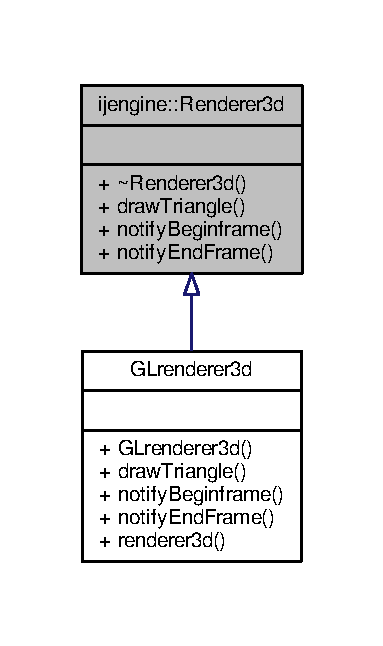
\includegraphics[width=184pt]{classijengine_1_1Renderer3d__inherit__graph}
\end{center}
\end{figure}


Collaboration diagram for ijengine\-:\-:Renderer3d\-:\nopagebreak
\begin{figure}[H]
\begin{center}
\leavevmode
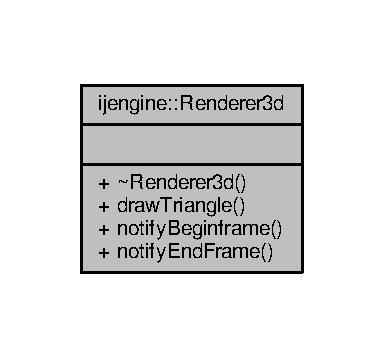
\includegraphics[width=184pt]{classijengine_1_1Renderer3d__coll__graph}
\end{center}
\end{figure}
\subsection*{Public Member Functions}
\begin{DoxyCompactItemize}
\item 
virtual \hyperlink{classijengine_1_1Renderer3d_a0c77a23b6ca21b49d976868df2618d7f}{$\sim$\-Renderer3d} ()=default
\item 
virtual void \hyperlink{classijengine_1_1Renderer3d_a105c5b22d90584aeda18cafdd15650da}{draw\-Triangle} (float x, float y, float z, float scale, int r, int g, int b)=0
\item 
virtual void \hyperlink{classijengine_1_1Renderer3d_a4f2d16d72f210445fdb9210b3fce33bf}{notify\-Beginframe} ()=0
\item 
virtual void \hyperlink{classijengine_1_1Renderer3d_af0a21ea9fc5ebd8e30922047bf743a14}{notify\-End\-Frame} ()=0
\end{DoxyCompactItemize}


\subsection{Constructor \& Destructor Documentation}
\hypertarget{classijengine_1_1Renderer3d_a0c77a23b6ca21b49d976868df2618d7f}{\index{ijengine\-::\-Renderer3d@{ijengine\-::\-Renderer3d}!$\sim$\-Renderer3d@{$\sim$\-Renderer3d}}
\index{$\sim$\-Renderer3d@{$\sim$\-Renderer3d}!ijengine::Renderer3d@{ijengine\-::\-Renderer3d}}
\subsubsection[{$\sim$\-Renderer3d}]{\setlength{\rightskip}{0pt plus 5cm}virtual ijengine\-::\-Renderer3d\-::$\sim$\-Renderer3d (
\begin{DoxyParamCaption}
{}
\end{DoxyParamCaption}
)\hspace{0.3cm}{\ttfamily [virtual]}, {\ttfamily [default]}}}\label{classijengine_1_1Renderer3d_a0c77a23b6ca21b49d976868df2618d7f}


\subsection{Member Function Documentation}
\hypertarget{classijengine_1_1Renderer3d_a105c5b22d90584aeda18cafdd15650da}{\index{ijengine\-::\-Renderer3d@{ijengine\-::\-Renderer3d}!draw\-Triangle@{draw\-Triangle}}
\index{draw\-Triangle@{draw\-Triangle}!ijengine::Renderer3d@{ijengine\-::\-Renderer3d}}
\subsubsection[{draw\-Triangle}]{\setlength{\rightskip}{0pt plus 5cm}virtual void ijengine\-::\-Renderer3d\-::draw\-Triangle (
\begin{DoxyParamCaption}
\item[{float}]{x, }
\item[{float}]{y, }
\item[{float}]{z, }
\item[{float}]{scale, }
\item[{int}]{r, }
\item[{int}]{g, }
\item[{int}]{b}
\end{DoxyParamCaption}
)\hspace{0.3cm}{\ttfamily [pure virtual]}}}\label{classijengine_1_1Renderer3d_a105c5b22d90584aeda18cafdd15650da}


Implemented in \hyperlink{classGLrenderer3d_af10dc480fc22622db6a83c87bb119ca7}{G\-Lrenderer3d}.

\hypertarget{classijengine_1_1Renderer3d_a4f2d16d72f210445fdb9210b3fce33bf}{\index{ijengine\-::\-Renderer3d@{ijengine\-::\-Renderer3d}!notify\-Beginframe@{notify\-Beginframe}}
\index{notify\-Beginframe@{notify\-Beginframe}!ijengine::Renderer3d@{ijengine\-::\-Renderer3d}}
\subsubsection[{notify\-Beginframe}]{\setlength{\rightskip}{0pt plus 5cm}virtual void ijengine\-::\-Renderer3d\-::notify\-Beginframe (
\begin{DoxyParamCaption}
{}
\end{DoxyParamCaption}
)\hspace{0.3cm}{\ttfamily [pure virtual]}}}\label{classijengine_1_1Renderer3d_a4f2d16d72f210445fdb9210b3fce33bf}


Implemented in \hyperlink{classGLrenderer3d_a69cfa7ad8eac36b068b8cc8e461d7c33}{G\-Lrenderer3d}.

\hypertarget{classijengine_1_1Renderer3d_af0a21ea9fc5ebd8e30922047bf743a14}{\index{ijengine\-::\-Renderer3d@{ijengine\-::\-Renderer3d}!notify\-End\-Frame@{notify\-End\-Frame}}
\index{notify\-End\-Frame@{notify\-End\-Frame}!ijengine::Renderer3d@{ijengine\-::\-Renderer3d}}
\subsubsection[{notify\-End\-Frame}]{\setlength{\rightskip}{0pt plus 5cm}virtual void ijengine\-::\-Renderer3d\-::notify\-End\-Frame (
\begin{DoxyParamCaption}
{}
\end{DoxyParamCaption}
)\hspace{0.3cm}{\ttfamily [pure virtual]}}}\label{classijengine_1_1Renderer3d_af0a21ea9fc5ebd8e30922047bf743a14}


Implemented in \hyperlink{classGLrenderer3d_a1625b7fa82863e7f54ba86d2ebe5f7af}{G\-Lrenderer3d}.



The documentation for this class was generated from the following file\-:\begin{DoxyCompactItemize}
\item 
/home/carla/git/ijengine-\/\-I\-C\-G\-\_\-\-G\-L/include/\hyperlink{renderer3d_8h}{renderer3d.\-h}\end{DoxyCompactItemize}

\hypertarget{classijengine_1_1SDL2Canvas}{\section{ijengine\-:\-:S\-D\-L2\-Canvas Class Reference}
\label{classijengine_1_1SDL2Canvas}\index{ijengine\-::\-S\-D\-L2\-Canvas@{ijengine\-::\-S\-D\-L2\-Canvas}}
}


{\ttfamily \#include $<$sdl2canvas.\-h$>$}



Inheritance diagram for ijengine\-:\-:S\-D\-L2\-Canvas\-:\nopagebreak
\begin{figure}[H]
\begin{center}
\leavevmode
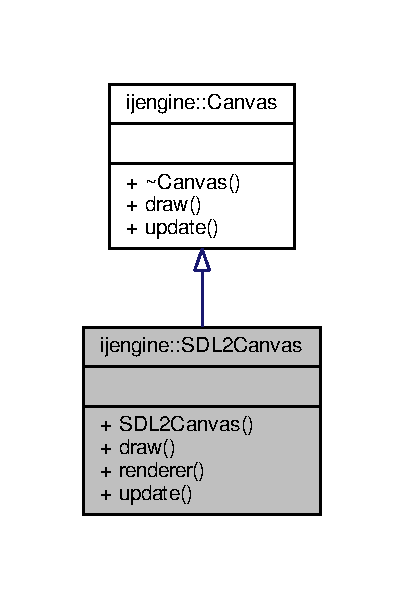
\includegraphics[width=194pt]{classijengine_1_1SDL2Canvas__inherit__graph}
\end{center}
\end{figure}


Collaboration diagram for ijengine\-:\-:S\-D\-L2\-Canvas\-:\nopagebreak
\begin{figure}[H]
\begin{center}
\leavevmode
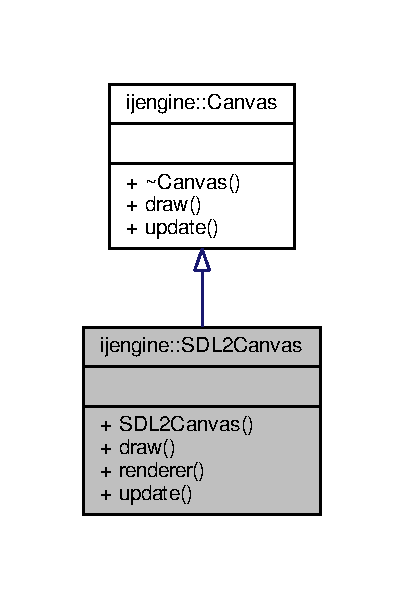
\includegraphics[width=194pt]{classijengine_1_1SDL2Canvas__coll__graph}
\end{center}
\end{figure}
\subsection*{Public Member Functions}
\begin{DoxyCompactItemize}
\item 
\hyperlink{classijengine_1_1SDL2Canvas_aa83ba37c30b25a0d4c8ca15d37f76e01}{S\-D\-L2\-Canvas} (S\-D\-L\-\_\-\-Renderer $\ast$\hyperlink{classijengine_1_1SDL2Canvas_a4c5237e37a864ede4242751732c4bc0b}{renderer})
\item 
void \hyperlink{classijengine_1_1SDL2Canvas_a764abc16a5bcdd6f0d1ab1c117839ee0}{draw} (const \hyperlink{classijengine_1_1Texture}{Texture} $\ast$texture, int x, int y)
\item 
S\-D\-L\-\_\-\-Renderer $\ast$ \hyperlink{classijengine_1_1SDL2Canvas_a4c5237e37a864ede4242751732c4bc0b}{renderer} () const 
\item 
void \hyperlink{classijengine_1_1SDL2Canvas_a5b87afff98211d159da84986f5b04e99}{update} ()
\end{DoxyCompactItemize}


\subsection{Constructor \& Destructor Documentation}
\hypertarget{classijengine_1_1SDL2Canvas_aa83ba37c30b25a0d4c8ca15d37f76e01}{\index{ijengine\-::\-S\-D\-L2\-Canvas@{ijengine\-::\-S\-D\-L2\-Canvas}!S\-D\-L2\-Canvas@{S\-D\-L2\-Canvas}}
\index{S\-D\-L2\-Canvas@{S\-D\-L2\-Canvas}!ijengine::SDL2Canvas@{ijengine\-::\-S\-D\-L2\-Canvas}}
\subsubsection[{S\-D\-L2\-Canvas}]{\setlength{\rightskip}{0pt plus 5cm}ijengine\-::\-S\-D\-L2\-Canvas\-::\-S\-D\-L2\-Canvas (
\begin{DoxyParamCaption}
\item[{S\-D\-L\-\_\-\-Renderer $\ast$}]{renderer}
\end{DoxyParamCaption}
)}}\label{classijengine_1_1SDL2Canvas_aa83ba37c30b25a0d4c8ca15d37f76e01}


\subsection{Member Function Documentation}
\hypertarget{classijengine_1_1SDL2Canvas_a764abc16a5bcdd6f0d1ab1c117839ee0}{\index{ijengine\-::\-S\-D\-L2\-Canvas@{ijengine\-::\-S\-D\-L2\-Canvas}!draw@{draw}}
\index{draw@{draw}!ijengine::SDL2Canvas@{ijengine\-::\-S\-D\-L2\-Canvas}}
\subsubsection[{draw}]{\setlength{\rightskip}{0pt plus 5cm}void ijengine\-::\-S\-D\-L2\-Canvas\-::draw (
\begin{DoxyParamCaption}
\item[{const {\bf Texture} $\ast$}]{texture, }
\item[{int}]{x, }
\item[{int}]{y}
\end{DoxyParamCaption}
)\hspace{0.3cm}{\ttfamily [virtual]}}}\label{classijengine_1_1SDL2Canvas_a764abc16a5bcdd6f0d1ab1c117839ee0}


Implements \hyperlink{classijengine_1_1Canvas_ad941145373d040fa6b3b6f65366aaafa}{ijengine\-::\-Canvas}.



Here is the call graph for this function\-:\nopagebreak
\begin{figure}[H]
\begin{center}
\leavevmode
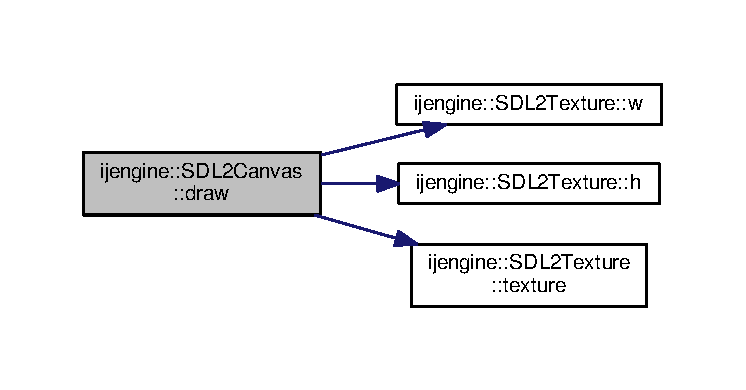
\includegraphics[width=350pt]{classijengine_1_1SDL2Canvas_a764abc16a5bcdd6f0d1ab1c117839ee0_cgraph}
\end{center}
\end{figure}


\hypertarget{classijengine_1_1SDL2Canvas_a4c5237e37a864ede4242751732c4bc0b}{\index{ijengine\-::\-S\-D\-L2\-Canvas@{ijengine\-::\-S\-D\-L2\-Canvas}!renderer@{renderer}}
\index{renderer@{renderer}!ijengine::SDL2Canvas@{ijengine\-::\-S\-D\-L2\-Canvas}}
\subsubsection[{renderer}]{\setlength{\rightskip}{0pt plus 5cm}S\-D\-L\-\_\-\-Renderer $\ast$ ijengine\-::\-S\-D\-L2\-Canvas\-::renderer (
\begin{DoxyParamCaption}
{}
\end{DoxyParamCaption}
) const}}\label{classijengine_1_1SDL2Canvas_a4c5237e37a864ede4242751732c4bc0b}
\hypertarget{classijengine_1_1SDL2Canvas_a5b87afff98211d159da84986f5b04e99}{\index{ijengine\-::\-S\-D\-L2\-Canvas@{ijengine\-::\-S\-D\-L2\-Canvas}!update@{update}}
\index{update@{update}!ijengine::SDL2Canvas@{ijengine\-::\-S\-D\-L2\-Canvas}}
\subsubsection[{update}]{\setlength{\rightskip}{0pt plus 5cm}void ijengine\-::\-S\-D\-L2\-Canvas\-::update (
\begin{DoxyParamCaption}
{}
\end{DoxyParamCaption}
)\hspace{0.3cm}{\ttfamily [virtual]}}}\label{classijengine_1_1SDL2Canvas_a5b87afff98211d159da84986f5b04e99}


Implements \hyperlink{classijengine_1_1Canvas_ad0f3aace5114a8cb2d457f0f272c6743}{ijengine\-::\-Canvas}.



The documentation for this class was generated from the following files\-:\begin{DoxyCompactItemize}
\item 
/home/carla/git/ijengine-\/\-I\-C\-G\-\_\-\-G\-L/include/\hyperlink{sdl2canvas_8h}{sdl2canvas.\-h}\item 
/home/carla/git/ijengine-\/\-I\-C\-G\-\_\-\-G\-L/src/\hyperlink{sdl2canvas_8cpp}{sdl2canvas.\-cpp}\end{DoxyCompactItemize}

\hypertarget{classijengine_1_1SDL2DVideo}{\section{ijengine\-:\-:S\-D\-L2\-D\-Video Class Reference}
\label{classijengine_1_1SDL2DVideo}\index{ijengine\-::\-S\-D\-L2\-D\-Video@{ijengine\-::\-S\-D\-L2\-D\-Video}}
}


{\ttfamily \#include $<$sdl2\-Dvideo.\-h$>$}



Inheritance diagram for ijengine\-:\-:S\-D\-L2\-D\-Video\-:\nopagebreak
\begin{figure}[H]
\begin{center}
\leavevmode
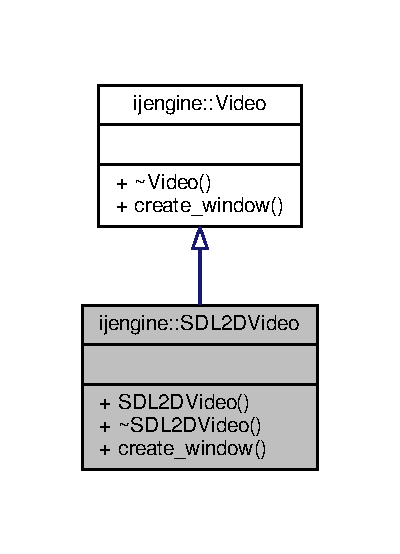
\includegraphics[width=192pt]{classijengine_1_1SDL2DVideo__inherit__graph}
\end{center}
\end{figure}


Collaboration diagram for ijengine\-:\-:S\-D\-L2\-D\-Video\-:\nopagebreak
\begin{figure}[H]
\begin{center}
\leavevmode
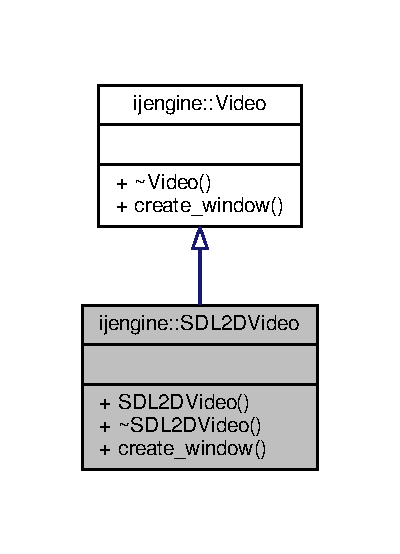
\includegraphics[width=192pt]{classijengine_1_1SDL2DVideo__coll__graph}
\end{center}
\end{figure}
\subsection*{Public Member Functions}
\begin{DoxyCompactItemize}
\item 
\hyperlink{classijengine_1_1SDL2DVideo_abced6545a0115b81dc9ab7bb234d79fc}{S\-D\-L2\-D\-Video} ()
\item 
\hyperlink{classijengine_1_1SDL2DVideo_abc44a3ee426ba4b202af08c5e4dc924c}{$\sim$\-S\-D\-L2\-D\-Video} ()
\item 
\hyperlink{classijengine_1_1Window}{Window} $\ast$ \hyperlink{classijengine_1_1SDL2DVideo_a560fb324f6dcc18936901d4c91fa8e89}{create\-\_\-window} (int w, int h)
\end{DoxyCompactItemize}


\subsection{Constructor \& Destructor Documentation}
\hypertarget{classijengine_1_1SDL2DVideo_abced6545a0115b81dc9ab7bb234d79fc}{\index{ijengine\-::\-S\-D\-L2\-D\-Video@{ijengine\-::\-S\-D\-L2\-D\-Video}!S\-D\-L2\-D\-Video@{S\-D\-L2\-D\-Video}}
\index{S\-D\-L2\-D\-Video@{S\-D\-L2\-D\-Video}!ijengine::SDL2DVideo@{ijengine\-::\-S\-D\-L2\-D\-Video}}
\subsubsection[{S\-D\-L2\-D\-Video}]{\setlength{\rightskip}{0pt plus 5cm}ijengine\-::\-S\-D\-L2\-D\-Video\-::\-S\-D\-L2\-D\-Video (
\begin{DoxyParamCaption}
{}
\end{DoxyParamCaption}
)}}\label{classijengine_1_1SDL2DVideo_abced6545a0115b81dc9ab7bb234d79fc}
\hypertarget{classijengine_1_1SDL2DVideo_abc44a3ee426ba4b202af08c5e4dc924c}{\index{ijengine\-::\-S\-D\-L2\-D\-Video@{ijengine\-::\-S\-D\-L2\-D\-Video}!$\sim$\-S\-D\-L2\-D\-Video@{$\sim$\-S\-D\-L2\-D\-Video}}
\index{$\sim$\-S\-D\-L2\-D\-Video@{$\sim$\-S\-D\-L2\-D\-Video}!ijengine::SDL2DVideo@{ijengine\-::\-S\-D\-L2\-D\-Video}}
\subsubsection[{$\sim$\-S\-D\-L2\-D\-Video}]{\setlength{\rightskip}{0pt plus 5cm}ijengine\-::\-S\-D\-L2\-D\-Video\-::$\sim$\-S\-D\-L2\-D\-Video (
\begin{DoxyParamCaption}
{}
\end{DoxyParamCaption}
)}}\label{classijengine_1_1SDL2DVideo_abc44a3ee426ba4b202af08c5e4dc924c}


\subsection{Member Function Documentation}
\hypertarget{classijengine_1_1SDL2DVideo_a560fb324f6dcc18936901d4c91fa8e89}{\index{ijengine\-::\-S\-D\-L2\-D\-Video@{ijengine\-::\-S\-D\-L2\-D\-Video}!create\-\_\-window@{create\-\_\-window}}
\index{create\-\_\-window@{create\-\_\-window}!ijengine::SDL2DVideo@{ijengine\-::\-S\-D\-L2\-D\-Video}}
\subsubsection[{create\-\_\-window}]{\setlength{\rightskip}{0pt plus 5cm}{\bf Window} $\ast$ ijengine\-::\-S\-D\-L2\-D\-Video\-::create\-\_\-window (
\begin{DoxyParamCaption}
\item[{int}]{w, }
\item[{int}]{h}
\end{DoxyParamCaption}
)\hspace{0.3cm}{\ttfamily [virtual]}}}\label{classijengine_1_1SDL2DVideo_a560fb324f6dcc18936901d4c91fa8e89}


Implements \hyperlink{classijengine_1_1Video_a21c552c463b2a7466394c2b6e7e1ca99}{ijengine\-::\-Video}.



The documentation for this class was generated from the following files\-:\begin{DoxyCompactItemize}
\item 
/home/carla/git/ijengine-\/\-I\-C\-G\-\_\-\-G\-L/include/\hyperlink{sdl2Dvideo_8h}{sdl2\-Dvideo.\-h}\item 
/home/carla/git/ijengine-\/\-I\-C\-G\-\_\-\-G\-L/src/\hyperlink{sdl2Dvideo_8cpp}{sdl2\-Dvideo.\-cpp}\end{DoxyCompactItemize}

\hypertarget{classijengine_1_1SDL2Game}{\section{ijengine\-:\-:S\-D\-L2\-Game Class Reference}
\label{classijengine_1_1SDL2Game}\index{ijengine\-::\-S\-D\-L2\-Game@{ijengine\-::\-S\-D\-L2\-Game}}
}


{\ttfamily \#include $<$sdl2game.\-h$>$}



Inheritance diagram for ijengine\-:\-:S\-D\-L2\-Game\-:\nopagebreak
\begin{figure}[H]
\begin{center}
\leavevmode
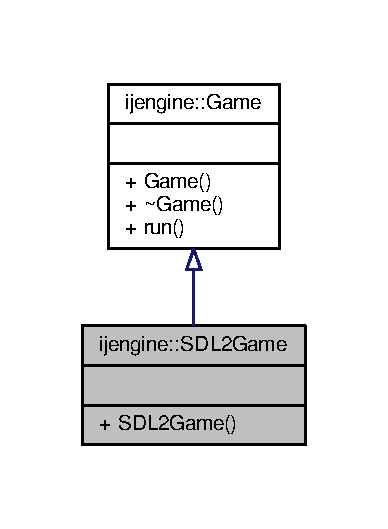
\includegraphics[width=186pt]{classijengine_1_1SDL2Game__inherit__graph}
\end{center}
\end{figure}


Collaboration diagram for ijengine\-:\-:S\-D\-L2\-Game\-:\nopagebreak
\begin{figure}[H]
\begin{center}
\leavevmode
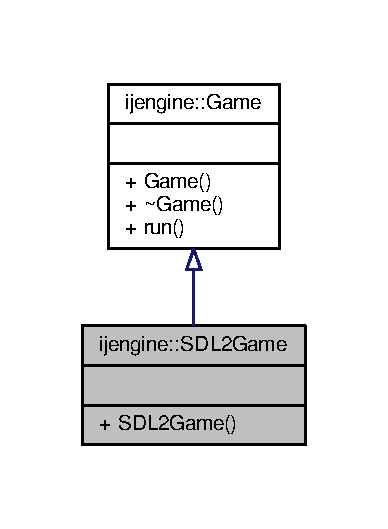
\includegraphics[width=186pt]{classijengine_1_1SDL2Game__coll__graph}
\end{center}
\end{figure}
\subsection*{Public Member Functions}
\begin{DoxyCompactItemize}
\item 
\hyperlink{classijengine_1_1SDL2Game_a85c10694ae6091b2979ed922a911adef}{S\-D\-L2\-Game} ()
\end{DoxyCompactItemize}


\subsection{Constructor \& Destructor Documentation}
\hypertarget{classijengine_1_1SDL2Game_a85c10694ae6091b2979ed922a911adef}{\index{ijengine\-::\-S\-D\-L2\-Game@{ijengine\-::\-S\-D\-L2\-Game}!S\-D\-L2\-Game@{S\-D\-L2\-Game}}
\index{S\-D\-L2\-Game@{S\-D\-L2\-Game}!ijengine::SDL2Game@{ijengine\-::\-S\-D\-L2\-Game}}
\subsubsection[{S\-D\-L2\-Game}]{\setlength{\rightskip}{0pt plus 5cm}ijengine\-::\-S\-D\-L2\-Game\-::\-S\-D\-L2\-Game (
\begin{DoxyParamCaption}
{}
\end{DoxyParamCaption}
)}}\label{classijengine_1_1SDL2Game_a85c10694ae6091b2979ed922a911adef}


Here is the call graph for this function\-:\nopagebreak
\begin{figure}[H]
\begin{center}
\leavevmode
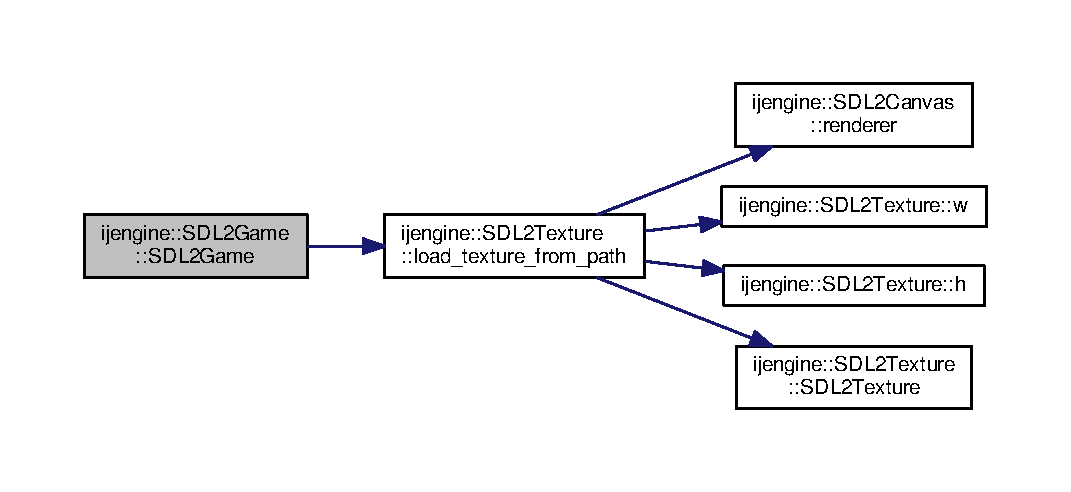
\includegraphics[width=350pt]{classijengine_1_1SDL2Game_a85c10694ae6091b2979ed922a911adef_cgraph}
\end{center}
\end{figure}




The documentation for this class was generated from the following files\-:\begin{DoxyCompactItemize}
\item 
/home/carla/git/ijengine-\/\-I\-C\-G\-\_\-\-G\-L/include/\hyperlink{sdl2game_8h}{sdl2game.\-h}\item 
/home/carla/git/ijengine-\/\-I\-C\-G\-\_\-\-G\-L/src/\hyperlink{sdl2game_8cpp}{sdl2game.\-cpp}\end{DoxyCompactItemize}

\hypertarget{classijengine_1_1SDL2Texture}{\section{ijengine\-:\-:S\-D\-L2\-Texture Class Reference}
\label{classijengine_1_1SDL2Texture}\index{ijengine\-::\-S\-D\-L2\-Texture@{ijengine\-::\-S\-D\-L2\-Texture}}
}


{\ttfamily \#include $<$sdl2texture.\-h$>$}



Inheritance diagram for ijengine\-:\-:S\-D\-L2\-Texture\-:\nopagebreak
\begin{figure}[H]
\begin{center}
\leavevmode
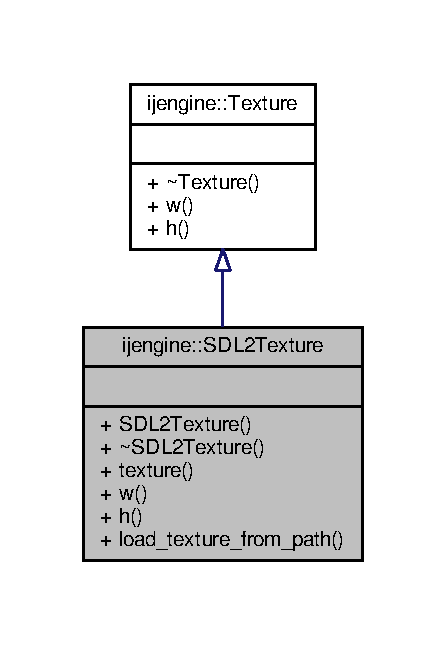
\includegraphics[width=214pt]{classijengine_1_1SDL2Texture__inherit__graph}
\end{center}
\end{figure}


Collaboration diagram for ijengine\-:\-:S\-D\-L2\-Texture\-:\nopagebreak
\begin{figure}[H]
\begin{center}
\leavevmode
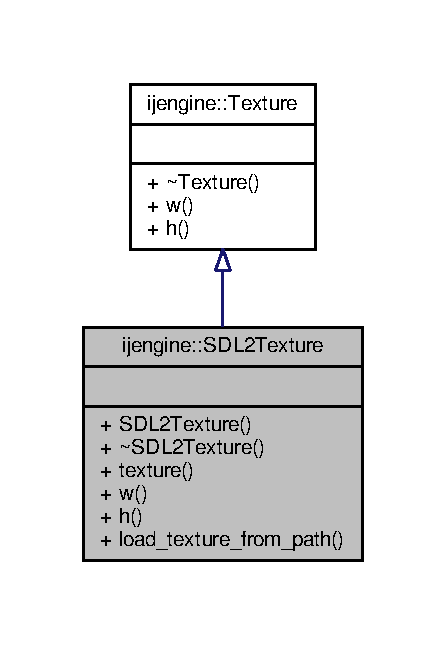
\includegraphics[width=214pt]{classijengine_1_1SDL2Texture__coll__graph}
\end{center}
\end{figure}
\subsection*{Public Member Functions}
\begin{DoxyCompactItemize}
\item 
\hyperlink{classijengine_1_1SDL2Texture_a4eb052ac3a431cc81cd2feba6aa65e67}{S\-D\-L2\-Texture} (S\-D\-L\-\_\-\-Texture $\ast$\hyperlink{classijengine_1_1SDL2Texture_ab2b7be6a96eb385b9695f358283f006c}{texture}, int \hyperlink{classijengine_1_1SDL2Texture_a94b43ffad7f1ea5ac74165e59085ffce}{w}, int \hyperlink{classijengine_1_1SDL2Texture_a5202ccb0ca2cd152fd3597b45235556e}{h})
\item 
\hyperlink{classijengine_1_1SDL2Texture_a18eb28859d46b9a918ff27b2f8a37501}{$\sim$\-S\-D\-L2\-Texture} ()
\item 
S\-D\-L\-\_\-\-Texture $\ast$ \hyperlink{classijengine_1_1SDL2Texture_ab2b7be6a96eb385b9695f358283f006c}{texture} () const 
\item 
int \hyperlink{classijengine_1_1SDL2Texture_a94b43ffad7f1ea5ac74165e59085ffce}{w} () const 
\item 
int \hyperlink{classijengine_1_1SDL2Texture_a5202ccb0ca2cd152fd3597b45235556e}{h} () const 
\end{DoxyCompactItemize}
\subsection*{Static Public Member Functions}
\begin{DoxyCompactItemize}
\item 
static \hyperlink{classijengine_1_1SDL2Texture}{S\-D\-L2\-Texture} $\ast$ \hyperlink{classijengine_1_1SDL2Texture_a2685a9df8d7152bc132990dea3ffe813}{load\-\_\-texture\-\_\-from\-\_\-path} (const string \&path, const \hyperlink{classijengine_1_1Canvas}{Canvas} $\ast$c)
\end{DoxyCompactItemize}


\subsection{Constructor \& Destructor Documentation}
\hypertarget{classijengine_1_1SDL2Texture_a4eb052ac3a431cc81cd2feba6aa65e67}{\index{ijengine\-::\-S\-D\-L2\-Texture@{ijengine\-::\-S\-D\-L2\-Texture}!S\-D\-L2\-Texture@{S\-D\-L2\-Texture}}
\index{S\-D\-L2\-Texture@{S\-D\-L2\-Texture}!ijengine::SDL2Texture@{ijengine\-::\-S\-D\-L2\-Texture}}
\subsubsection[{S\-D\-L2\-Texture}]{\setlength{\rightskip}{0pt plus 5cm}ijengine\-::\-S\-D\-L2\-Texture\-::\-S\-D\-L2\-Texture (
\begin{DoxyParamCaption}
\item[{S\-D\-L\-\_\-\-Texture $\ast$}]{texture, }
\item[{int}]{w, }
\item[{int}]{h}
\end{DoxyParamCaption}
)}}\label{classijengine_1_1SDL2Texture_a4eb052ac3a431cc81cd2feba6aa65e67}
\hypertarget{classijengine_1_1SDL2Texture_a18eb28859d46b9a918ff27b2f8a37501}{\index{ijengine\-::\-S\-D\-L2\-Texture@{ijengine\-::\-S\-D\-L2\-Texture}!$\sim$\-S\-D\-L2\-Texture@{$\sim$\-S\-D\-L2\-Texture}}
\index{$\sim$\-S\-D\-L2\-Texture@{$\sim$\-S\-D\-L2\-Texture}!ijengine::SDL2Texture@{ijengine\-::\-S\-D\-L2\-Texture}}
\subsubsection[{$\sim$\-S\-D\-L2\-Texture}]{\setlength{\rightskip}{0pt plus 5cm}ijengine\-::\-S\-D\-L2\-Texture\-::$\sim$\-S\-D\-L2\-Texture (
\begin{DoxyParamCaption}
{}
\end{DoxyParamCaption}
)}}\label{classijengine_1_1SDL2Texture_a18eb28859d46b9a918ff27b2f8a37501}


\subsection{Member Function Documentation}
\hypertarget{classijengine_1_1SDL2Texture_a5202ccb0ca2cd152fd3597b45235556e}{\index{ijengine\-::\-S\-D\-L2\-Texture@{ijengine\-::\-S\-D\-L2\-Texture}!h@{h}}
\index{h@{h}!ijengine::SDL2Texture@{ijengine\-::\-S\-D\-L2\-Texture}}
\subsubsection[{h}]{\setlength{\rightskip}{0pt plus 5cm}int ijengine\-::\-S\-D\-L2\-Texture\-::h (
\begin{DoxyParamCaption}
{}
\end{DoxyParamCaption}
) const\hspace{0.3cm}{\ttfamily [inline]}, {\ttfamily [virtual]}}}\label{classijengine_1_1SDL2Texture_a5202ccb0ca2cd152fd3597b45235556e}


Implements \hyperlink{classijengine_1_1Texture_a9ffe6059a07f4f20251578d9d9f9334c}{ijengine\-::\-Texture}.

\hypertarget{classijengine_1_1SDL2Texture_a2685a9df8d7152bc132990dea3ffe813}{\index{ijengine\-::\-S\-D\-L2\-Texture@{ijengine\-::\-S\-D\-L2\-Texture}!load\-\_\-texture\-\_\-from\-\_\-path@{load\-\_\-texture\-\_\-from\-\_\-path}}
\index{load\-\_\-texture\-\_\-from\-\_\-path@{load\-\_\-texture\-\_\-from\-\_\-path}!ijengine::SDL2Texture@{ijengine\-::\-S\-D\-L2\-Texture}}
\subsubsection[{load\-\_\-texture\-\_\-from\-\_\-path}]{\setlength{\rightskip}{0pt plus 5cm}{\bf S\-D\-L2\-Texture} $\ast$ ijengine\-::\-S\-D\-L2\-Texture\-::load\-\_\-texture\-\_\-from\-\_\-path (
\begin{DoxyParamCaption}
\item[{const string \&}]{path, }
\item[{const {\bf Canvas} $\ast$}]{c}
\end{DoxyParamCaption}
)\hspace{0.3cm}{\ttfamily [static]}}}\label{classijengine_1_1SDL2Texture_a2685a9df8d7152bc132990dea3ffe813}


Here is the call graph for this function\-:\nopagebreak
\begin{figure}[H]
\begin{center}
\leavevmode
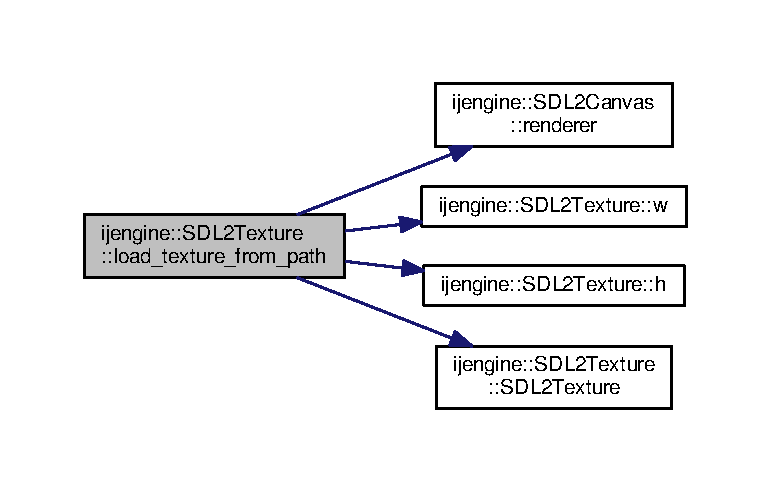
\includegraphics[width=350pt]{classijengine_1_1SDL2Texture_a2685a9df8d7152bc132990dea3ffe813_cgraph}
\end{center}
\end{figure}


\hypertarget{classijengine_1_1SDL2Texture_ab2b7be6a96eb385b9695f358283f006c}{\index{ijengine\-::\-S\-D\-L2\-Texture@{ijengine\-::\-S\-D\-L2\-Texture}!texture@{texture}}
\index{texture@{texture}!ijengine::SDL2Texture@{ijengine\-::\-S\-D\-L2\-Texture}}
\subsubsection[{texture}]{\setlength{\rightskip}{0pt plus 5cm}S\-D\-L\-\_\-\-Texture $\ast$ ijengine\-::\-S\-D\-L2\-Texture\-::texture (
\begin{DoxyParamCaption}
{}
\end{DoxyParamCaption}
) const}}\label{classijengine_1_1SDL2Texture_ab2b7be6a96eb385b9695f358283f006c}
\hypertarget{classijengine_1_1SDL2Texture_a94b43ffad7f1ea5ac74165e59085ffce}{\index{ijengine\-::\-S\-D\-L2\-Texture@{ijengine\-::\-S\-D\-L2\-Texture}!w@{w}}
\index{w@{w}!ijengine::SDL2Texture@{ijengine\-::\-S\-D\-L2\-Texture}}
\subsubsection[{w}]{\setlength{\rightskip}{0pt plus 5cm}int ijengine\-::\-S\-D\-L2\-Texture\-::w (
\begin{DoxyParamCaption}
{}
\end{DoxyParamCaption}
) const\hspace{0.3cm}{\ttfamily [inline]}, {\ttfamily [virtual]}}}\label{classijengine_1_1SDL2Texture_a94b43ffad7f1ea5ac74165e59085ffce}


Implements \hyperlink{classijengine_1_1Texture_a8de34c2971f12e08d49c5f51d8236178}{ijengine\-::\-Texture}.



The documentation for this class was generated from the following files\-:\begin{DoxyCompactItemize}
\item 
/home/carla/git/ijengine-\/\-I\-C\-G\-\_\-\-G\-L/include/\hyperlink{sdl2texture_8h}{sdl2texture.\-h}\item 
/home/carla/git/ijengine-\/\-I\-C\-G\-\_\-\-G\-L/src/\hyperlink{sdl2texture_8cpp}{sdl2texture.\-cpp}\end{DoxyCompactItemize}

\hypertarget{classijengine_1_1SDL2Window}{\section{ijengine\-:\-:S\-D\-L2\-Window Class Reference}
\label{classijengine_1_1SDL2Window}\index{ijengine\-::\-S\-D\-L2\-Window@{ijengine\-::\-S\-D\-L2\-Window}}
}


{\ttfamily \#include $<$sdl2window.\-h$>$}



Inheritance diagram for ijengine\-:\-:S\-D\-L2\-Window\-:\nopagebreak
\begin{figure}[H]
\begin{center}
\leavevmode
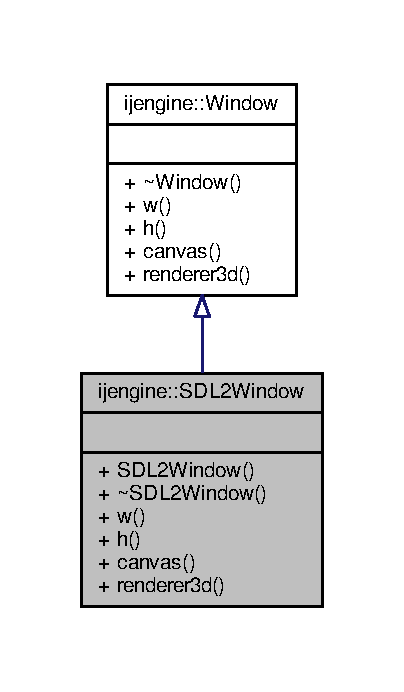
\includegraphics[width=194pt]{classijengine_1_1SDL2Window__inherit__graph}
\end{center}
\end{figure}


Collaboration diagram for ijengine\-:\-:S\-D\-L2\-Window\-:\nopagebreak
\begin{figure}[H]
\begin{center}
\leavevmode
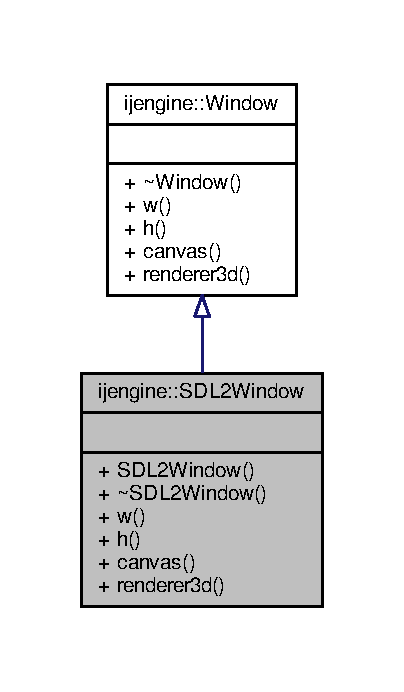
\includegraphics[width=194pt]{classijengine_1_1SDL2Window__coll__graph}
\end{center}
\end{figure}
\subsection*{Public Member Functions}
\begin{DoxyCompactItemize}
\item 
\hyperlink{classijengine_1_1SDL2Window_ae49b726543bf75c4ef88577873c0b595}{S\-D\-L2\-Window} (S\-D\-L\-\_\-\-Window $\ast$window, S\-D\-L\-\_\-\-Renderer $\ast$renderer)
\item 
\hyperlink{classijengine_1_1SDL2Window_adacbfc303f24217bbcffeadfe0196a16}{$\sim$\-S\-D\-L2\-Window} ()
\item 
int \hyperlink{classijengine_1_1SDL2Window_a9ee858781f682de6e1f4e07e0e005d52}{w} () const 
\item 
int \hyperlink{classijengine_1_1SDL2Window_a22bfc90a19791ec62bee093b573a1317}{h} () const 
\item 
\hyperlink{classijengine_1_1Canvas}{Canvas} $\ast$ \hyperlink{classijengine_1_1SDL2Window_a67813fe0b83700d046a4b84112b9ceb3}{canvas} () const 
\item 
\hyperlink{classijengine_1_1Renderer3d}{Renderer3d} $\ast$ \hyperlink{classijengine_1_1SDL2Window_aa35b142bef03f2fd5fc17382bfef39f1}{renderer3d} () const 
\end{DoxyCompactItemize}


\subsection{Constructor \& Destructor Documentation}
\hypertarget{classijengine_1_1SDL2Window_ae49b726543bf75c4ef88577873c0b595}{\index{ijengine\-::\-S\-D\-L2\-Window@{ijengine\-::\-S\-D\-L2\-Window}!S\-D\-L2\-Window@{S\-D\-L2\-Window}}
\index{S\-D\-L2\-Window@{S\-D\-L2\-Window}!ijengine::SDL2Window@{ijengine\-::\-S\-D\-L2\-Window}}
\subsubsection[{S\-D\-L2\-Window}]{\setlength{\rightskip}{0pt plus 5cm}ijengine\-::\-S\-D\-L2\-Window\-::\-S\-D\-L2\-Window (
\begin{DoxyParamCaption}
\item[{S\-D\-L\-\_\-\-Window $\ast$}]{window, }
\item[{S\-D\-L\-\_\-\-Renderer $\ast$}]{renderer}
\end{DoxyParamCaption}
)}}\label{classijengine_1_1SDL2Window_ae49b726543bf75c4ef88577873c0b595}
\hypertarget{classijengine_1_1SDL2Window_adacbfc303f24217bbcffeadfe0196a16}{\index{ijengine\-::\-S\-D\-L2\-Window@{ijengine\-::\-S\-D\-L2\-Window}!$\sim$\-S\-D\-L2\-Window@{$\sim$\-S\-D\-L2\-Window}}
\index{$\sim$\-S\-D\-L2\-Window@{$\sim$\-S\-D\-L2\-Window}!ijengine::SDL2Window@{ijengine\-::\-S\-D\-L2\-Window}}
\subsubsection[{$\sim$\-S\-D\-L2\-Window}]{\setlength{\rightskip}{0pt plus 5cm}ijengine\-::\-S\-D\-L2\-Window\-::$\sim$\-S\-D\-L2\-Window (
\begin{DoxyParamCaption}
{}
\end{DoxyParamCaption}
)}}\label{classijengine_1_1SDL2Window_adacbfc303f24217bbcffeadfe0196a16}


\subsection{Member Function Documentation}
\hypertarget{classijengine_1_1SDL2Window_a67813fe0b83700d046a4b84112b9ceb3}{\index{ijengine\-::\-S\-D\-L2\-Window@{ijengine\-::\-S\-D\-L2\-Window}!canvas@{canvas}}
\index{canvas@{canvas}!ijengine::SDL2Window@{ijengine\-::\-S\-D\-L2\-Window}}
\subsubsection[{canvas}]{\setlength{\rightskip}{0pt plus 5cm}{\bf Canvas} $\ast$ ijengine\-::\-S\-D\-L2\-Window\-::canvas (
\begin{DoxyParamCaption}
{}
\end{DoxyParamCaption}
) const\hspace{0.3cm}{\ttfamily [virtual]}}}\label{classijengine_1_1SDL2Window_a67813fe0b83700d046a4b84112b9ceb3}


Implements \hyperlink{classijengine_1_1Window_ad09bf41db3b3c65bdaaebb1986eee285}{ijengine\-::\-Window}.

\hypertarget{classijengine_1_1SDL2Window_a22bfc90a19791ec62bee093b573a1317}{\index{ijengine\-::\-S\-D\-L2\-Window@{ijengine\-::\-S\-D\-L2\-Window}!h@{h}}
\index{h@{h}!ijengine::SDL2Window@{ijengine\-::\-S\-D\-L2\-Window}}
\subsubsection[{h}]{\setlength{\rightskip}{0pt plus 5cm}int ijengine\-::\-S\-D\-L2\-Window\-::h (
\begin{DoxyParamCaption}
{}
\end{DoxyParamCaption}
) const\hspace{0.3cm}{\ttfamily [virtual]}}}\label{classijengine_1_1SDL2Window_a22bfc90a19791ec62bee093b573a1317}


Implements \hyperlink{classijengine_1_1Window_a1f77cd9da190853e8721a2f18bc2ffba}{ijengine\-::\-Window}.

\hypertarget{classijengine_1_1SDL2Window_aa35b142bef03f2fd5fc17382bfef39f1}{\index{ijengine\-::\-S\-D\-L2\-Window@{ijengine\-::\-S\-D\-L2\-Window}!renderer3d@{renderer3d}}
\index{renderer3d@{renderer3d}!ijengine::SDL2Window@{ijengine\-::\-S\-D\-L2\-Window}}
\subsubsection[{renderer3d}]{\setlength{\rightskip}{0pt plus 5cm}{\bf Renderer3d} $\ast$ ijengine\-::\-S\-D\-L2\-Window\-::renderer3d (
\begin{DoxyParamCaption}
{}
\end{DoxyParamCaption}
) const\hspace{0.3cm}{\ttfamily [virtual]}}}\label{classijengine_1_1SDL2Window_aa35b142bef03f2fd5fc17382bfef39f1}


Implements \hyperlink{classijengine_1_1Window_aaa4026b334e10318ec1ea92bf62a4a90}{ijengine\-::\-Window}.

\hypertarget{classijengine_1_1SDL2Window_a9ee858781f682de6e1f4e07e0e005d52}{\index{ijengine\-::\-S\-D\-L2\-Window@{ijengine\-::\-S\-D\-L2\-Window}!w@{w}}
\index{w@{w}!ijengine::SDL2Window@{ijengine\-::\-S\-D\-L2\-Window}}
\subsubsection[{w}]{\setlength{\rightskip}{0pt plus 5cm}int ijengine\-::\-S\-D\-L2\-Window\-::w (
\begin{DoxyParamCaption}
{}
\end{DoxyParamCaption}
) const\hspace{0.3cm}{\ttfamily [virtual]}}}\label{classijengine_1_1SDL2Window_a9ee858781f682de6e1f4e07e0e005d52}


Implements \hyperlink{classijengine_1_1Window_a0481e6a3e12e4455cbc7205bcb7507de}{ijengine\-::\-Window}.



The documentation for this class was generated from the following files\-:\begin{DoxyCompactItemize}
\item 
/home/carla/git/ijengine-\/\-I\-C\-G\-\_\-\-G\-L/include/\hyperlink{sdl2window_8h}{sdl2window.\-h}\item 
/home/carla/git/ijengine-\/\-I\-C\-G\-\_\-\-G\-L/src/\hyperlink{sdl2window_8cpp}{sdl2window.\-cpp}\end{DoxyCompactItemize}

\hypertarget{classijengine_1_1SDL3DVideo}{\section{ijengine\-:\-:S\-D\-L3\-D\-Video Class Reference}
\label{classijengine_1_1SDL3DVideo}\index{ijengine\-::\-S\-D\-L3\-D\-Video@{ijengine\-::\-S\-D\-L3\-D\-Video}}
}


{\ttfamily \#include $<$sdl3\-Dvideo.\-h$>$}



Inheritance diagram for ijengine\-:\-:S\-D\-L3\-D\-Video\-:\nopagebreak
\begin{figure}[H]
\begin{center}
\leavevmode
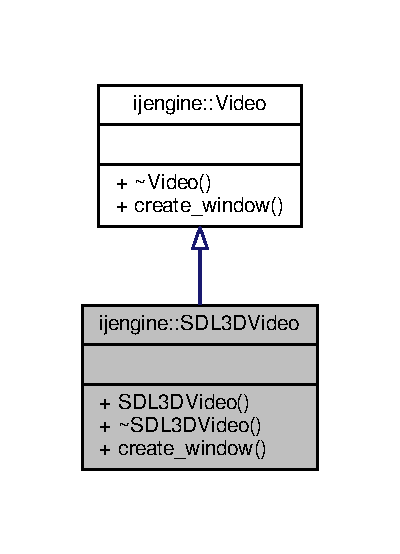
\includegraphics[width=192pt]{classijengine_1_1SDL3DVideo__inherit__graph}
\end{center}
\end{figure}


Collaboration diagram for ijengine\-:\-:S\-D\-L3\-D\-Video\-:\nopagebreak
\begin{figure}[H]
\begin{center}
\leavevmode
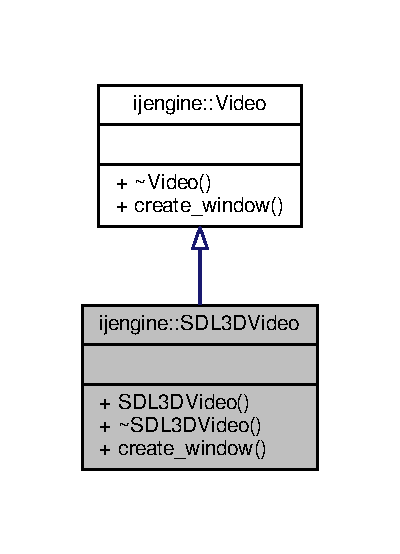
\includegraphics[width=192pt]{classijengine_1_1SDL3DVideo__coll__graph}
\end{center}
\end{figure}
\subsection*{Public Member Functions}
\begin{DoxyCompactItemize}
\item 
\hyperlink{classijengine_1_1SDL3DVideo_a298c059220a3e9f7c67360928c01a1b4}{S\-D\-L3\-D\-Video} ()
\item 
\hyperlink{classijengine_1_1SDL3DVideo_a1cdfbca736693c872d8302db5e6e6dda}{$\sim$\-S\-D\-L3\-D\-Video} ()
\item 
\hyperlink{classijengine_1_1Window}{Window} $\ast$ \hyperlink{classijengine_1_1SDL3DVideo_a91129138ce05c6d1f453f7cc854dba3f}{create\-\_\-window} (int w, int h)
\end{DoxyCompactItemize}


\subsection{Constructor \& Destructor Documentation}
\hypertarget{classijengine_1_1SDL3DVideo_a298c059220a3e9f7c67360928c01a1b4}{\index{ijengine\-::\-S\-D\-L3\-D\-Video@{ijengine\-::\-S\-D\-L3\-D\-Video}!S\-D\-L3\-D\-Video@{S\-D\-L3\-D\-Video}}
\index{S\-D\-L3\-D\-Video@{S\-D\-L3\-D\-Video}!ijengine::SDL3DVideo@{ijengine\-::\-S\-D\-L3\-D\-Video}}
\subsubsection[{S\-D\-L3\-D\-Video}]{\setlength{\rightskip}{0pt plus 5cm}ijengine\-::\-S\-D\-L3\-D\-Video\-::\-S\-D\-L3\-D\-Video (
\begin{DoxyParamCaption}
{}
\end{DoxyParamCaption}
)}}\label{classijengine_1_1SDL3DVideo_a298c059220a3e9f7c67360928c01a1b4}
\hypertarget{classijengine_1_1SDL3DVideo_a1cdfbca736693c872d8302db5e6e6dda}{\index{ijengine\-::\-S\-D\-L3\-D\-Video@{ijengine\-::\-S\-D\-L3\-D\-Video}!$\sim$\-S\-D\-L3\-D\-Video@{$\sim$\-S\-D\-L3\-D\-Video}}
\index{$\sim$\-S\-D\-L3\-D\-Video@{$\sim$\-S\-D\-L3\-D\-Video}!ijengine::SDL3DVideo@{ijengine\-::\-S\-D\-L3\-D\-Video}}
\subsubsection[{$\sim$\-S\-D\-L3\-D\-Video}]{\setlength{\rightskip}{0pt plus 5cm}ijengine\-::\-S\-D\-L3\-D\-Video\-::$\sim$\-S\-D\-L3\-D\-Video (
\begin{DoxyParamCaption}
{}
\end{DoxyParamCaption}
)}}\label{classijengine_1_1SDL3DVideo_a1cdfbca736693c872d8302db5e6e6dda}


\subsection{Member Function Documentation}
\hypertarget{classijengine_1_1SDL3DVideo_a91129138ce05c6d1f453f7cc854dba3f}{\index{ijengine\-::\-S\-D\-L3\-D\-Video@{ijengine\-::\-S\-D\-L3\-D\-Video}!create\-\_\-window@{create\-\_\-window}}
\index{create\-\_\-window@{create\-\_\-window}!ijengine::SDL3DVideo@{ijengine\-::\-S\-D\-L3\-D\-Video}}
\subsubsection[{create\-\_\-window}]{\setlength{\rightskip}{0pt plus 5cm}{\bf Window} $\ast$ ijengine\-::\-S\-D\-L3\-D\-Video\-::create\-\_\-window (
\begin{DoxyParamCaption}
\item[{int}]{w, }
\item[{int}]{h}
\end{DoxyParamCaption}
)\hspace{0.3cm}{\ttfamily [virtual]}}}\label{classijengine_1_1SDL3DVideo_a91129138ce05c6d1f453f7cc854dba3f}


Implements \hyperlink{classijengine_1_1Video_a21c552c463b2a7466394c2b6e7e1ca99}{ijengine\-::\-Video}.



The documentation for this class was generated from the following files\-:\begin{DoxyCompactItemize}
\item 
/home/carla/git/ijengine-\/\-I\-C\-G\-\_\-\-G\-L/include/\hyperlink{sdl3Dvideo_8h}{sdl3\-Dvideo.\-h}\item 
/home/carla/git/ijengine-\/\-I\-C\-G\-\_\-\-G\-L/src/\hyperlink{sdl3Dvideo_8cpp}{sdl3\-Dvideo.\-cpp}\end{DoxyCompactItemize}

\hypertarget{classijengine_1_1SDLGLGame}{\section{ijengine\-:\-:S\-D\-L\-G\-L\-Game Class Reference}
\label{classijengine_1_1SDLGLGame}\index{ijengine\-::\-S\-D\-L\-G\-L\-Game@{ijengine\-::\-S\-D\-L\-G\-L\-Game}}
}


{\ttfamily \#include $<$sdlglgame.\-h$>$}



Inheritance diagram for ijengine\-:\-:S\-D\-L\-G\-L\-Game\-:\nopagebreak
\begin{figure}[H]
\begin{center}
\leavevmode
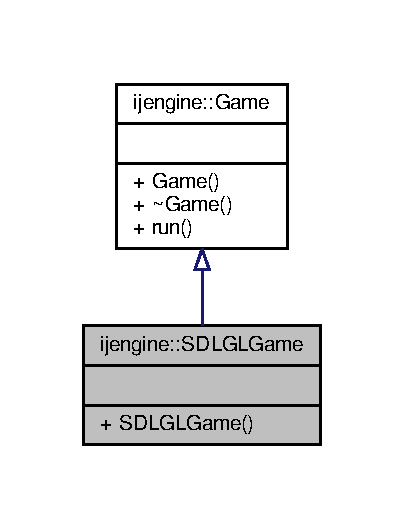
\includegraphics[width=194pt]{classijengine_1_1SDLGLGame__inherit__graph}
\end{center}
\end{figure}


Collaboration diagram for ijengine\-:\-:S\-D\-L\-G\-L\-Game\-:\nopagebreak
\begin{figure}[H]
\begin{center}
\leavevmode
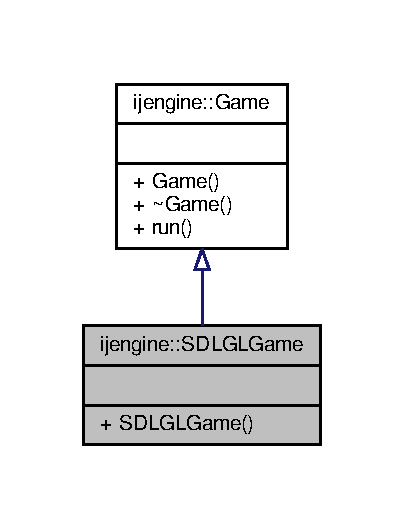
\includegraphics[width=194pt]{classijengine_1_1SDLGLGame__coll__graph}
\end{center}
\end{figure}
\subsection*{Public Member Functions}
\begin{DoxyCompactItemize}
\item 
\hyperlink{classijengine_1_1SDLGLGame_a12121059a5b887fefc5c636f1e6ce7fb}{S\-D\-L\-G\-L\-Game} ()
\end{DoxyCompactItemize}


\subsection{Constructor \& Destructor Documentation}
\hypertarget{classijengine_1_1SDLGLGame_a12121059a5b887fefc5c636f1e6ce7fb}{\index{ijengine\-::\-S\-D\-L\-G\-L\-Game@{ijengine\-::\-S\-D\-L\-G\-L\-Game}!S\-D\-L\-G\-L\-Game@{S\-D\-L\-G\-L\-Game}}
\index{S\-D\-L\-G\-L\-Game@{S\-D\-L\-G\-L\-Game}!ijengine::SDLGLGame@{ijengine\-::\-S\-D\-L\-G\-L\-Game}}
\subsubsection[{S\-D\-L\-G\-L\-Game}]{\setlength{\rightskip}{0pt plus 5cm}ijengine\-::\-S\-D\-L\-G\-L\-Game\-::\-S\-D\-L\-G\-L\-Game (
\begin{DoxyParamCaption}
{}
\end{DoxyParamCaption}
)}}\label{classijengine_1_1SDLGLGame_a12121059a5b887fefc5c636f1e6ce7fb}


The documentation for this class was generated from the following files\-:\begin{DoxyCompactItemize}
\item 
/home/carla/git/ijengine-\/\-I\-C\-G\-\_\-\-G\-L/include/\hyperlink{sdlglgame_8h}{sdlglgame.\-h}\item 
/home/carla/git/ijengine-\/\-I\-C\-G\-\_\-\-G\-L/src/\hyperlink{sdlglgame_8cpp}{sdlglgame.\-cpp}\end{DoxyCompactItemize}

\hypertarget{classijengine_1_1ShaderLoader}{\section{ijengine\-:\-:Shader\-Loader Class Reference}
\label{classijengine_1_1ShaderLoader}\index{ijengine\-::\-Shader\-Loader@{ijengine\-::\-Shader\-Loader}}
}


{\ttfamily \#include $<$shaderloader.\-h$>$}



Collaboration diagram for ijengine\-:\-:Shader\-Loader\-:\nopagebreak
\begin{figure}[H]
\begin{center}
\leavevmode
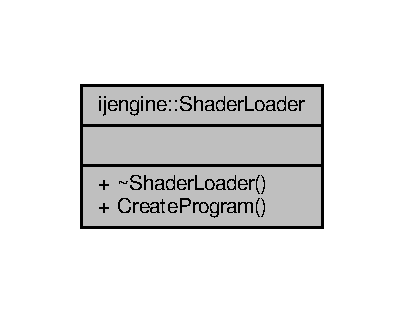
\includegraphics[width=194pt]{classijengine_1_1ShaderLoader__coll__graph}
\end{center}
\end{figure}
\subsection*{Public Member Functions}
\begin{DoxyCompactItemize}
\item 
virtual \hyperlink{classijengine_1_1ShaderLoader_a2a1f3389a09fadb89db8a7f4a291abf9}{$\sim$\-Shader\-Loader} ()
\item 
virtual void \hyperlink{classijengine_1_1ShaderLoader_ae9eaccd86333f426b7e569d51628fae5}{Create\-Program} (char $\ast$Shader\-Name, char $\ast$Vertex\-Shader\-File\-Name, char $\ast$Fragment\-Shader\-File\-Name)
\end{DoxyCompactItemize}


\subsection{Constructor \& Destructor Documentation}
\hypertarget{classijengine_1_1ShaderLoader_a2a1f3389a09fadb89db8a7f4a291abf9}{\index{ijengine\-::\-Shader\-Loader@{ijengine\-::\-Shader\-Loader}!$\sim$\-Shader\-Loader@{$\sim$\-Shader\-Loader}}
\index{$\sim$\-Shader\-Loader@{$\sim$\-Shader\-Loader}!ijengine::ShaderLoader@{ijengine\-::\-Shader\-Loader}}
\subsubsection[{$\sim$\-Shader\-Loader}]{\setlength{\rightskip}{0pt plus 5cm}virtual ijengine\-::\-Shader\-Loader\-::$\sim$\-Shader\-Loader (
\begin{DoxyParamCaption}
{}
\end{DoxyParamCaption}
)\hspace{0.3cm}{\ttfamily [virtual]}}}\label{classijengine_1_1ShaderLoader_a2a1f3389a09fadb89db8a7f4a291abf9}


\subsection{Member Function Documentation}
\hypertarget{classijengine_1_1ShaderLoader_ae9eaccd86333f426b7e569d51628fae5}{\index{ijengine\-::\-Shader\-Loader@{ijengine\-::\-Shader\-Loader}!Create\-Program@{Create\-Program}}
\index{Create\-Program@{Create\-Program}!ijengine::ShaderLoader@{ijengine\-::\-Shader\-Loader}}
\subsubsection[{Create\-Program}]{\setlength{\rightskip}{0pt plus 5cm}virtual void ijengine\-::\-Shader\-Loader\-::\-Create\-Program (
\begin{DoxyParamCaption}
\item[{char $\ast$}]{Shader\-Name, }
\item[{char $\ast$}]{Vertex\-Shader\-File\-Name, }
\item[{char $\ast$}]{Fragment\-Shader\-File\-Name}
\end{DoxyParamCaption}
)\hspace{0.3cm}{\ttfamily [virtual]}}}\label{classijengine_1_1ShaderLoader_ae9eaccd86333f426b7e569d51628fae5}


The documentation for this class was generated from the following file\-:\begin{DoxyCompactItemize}
\item 
/home/carla/git/ijengine-\/\-I\-C\-G\-\_\-\-G\-L/include/\hyperlink{shaderloader_8h}{shaderloader.\-h}\end{DoxyCompactItemize}

\hypertarget{classijengine_1_1ShaderManager}{\section{ijengine\-:\-:Shader\-Manager Class Reference}
\label{classijengine_1_1ShaderManager}\index{ijengine\-::\-Shader\-Manager@{ijengine\-::\-Shader\-Manager}}
}


{\ttfamily \#include $<$shader\-\_\-manager.\-h$>$}



Collaboration diagram for ijengine\-:\-:Shader\-Manager\-:\nopagebreak
\begin{figure}[H]
\begin{center}
\leavevmode
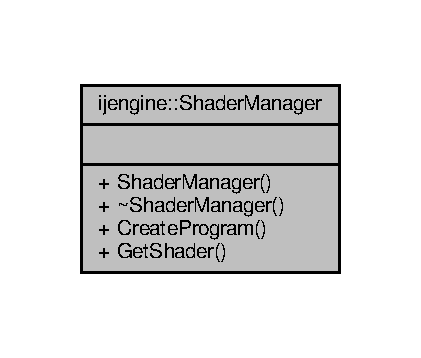
\includegraphics[width=202pt]{classijengine_1_1ShaderManager__coll__graph}
\end{center}
\end{figure}
\subsection*{Public Member Functions}
\begin{DoxyCompactItemize}
\item 
\hyperlink{classijengine_1_1ShaderManager_a7b64c6ab11f1ccb9b95c4bf59248d89c}{Shader\-Manager} ()
\item 
\hyperlink{classijengine_1_1ShaderManager_acfbc54fa76975c320a8078545a47a8a9}{$\sim$\-Shader\-Manager} ()
\item 
void \hyperlink{classijengine_1_1ShaderManager_a50a52860e644dada1fd3abac162a2c6e}{Create\-Program} (char $\ast$Shader\-Name, char $\ast$Vertex\-Shader\-File\-Name, char $\ast$Fragment\-Shader\-File\-Name)
\end{DoxyCompactItemize}
\subsection*{Static Public Member Functions}
\begin{DoxyCompactItemize}
\item 
static const G\-Luint \hyperlink{classijengine_1_1ShaderManager_acd75e97fa36a888d515e2c2c8552a3d1}{Get\-Shader} (const string \&shader\-Name)
\end{DoxyCompactItemize}


\subsection{Constructor \& Destructor Documentation}
\hypertarget{classijengine_1_1ShaderManager_a7b64c6ab11f1ccb9b95c4bf59248d89c}{\index{ijengine\-::\-Shader\-Manager@{ijengine\-::\-Shader\-Manager}!Shader\-Manager@{Shader\-Manager}}
\index{Shader\-Manager@{Shader\-Manager}!ijengine::ShaderManager@{ijengine\-::\-Shader\-Manager}}
\subsubsection[{Shader\-Manager}]{\setlength{\rightskip}{0pt plus 5cm}ijengine\-::\-Shader\-Manager\-::\-Shader\-Manager (
\begin{DoxyParamCaption}
{}
\end{DoxyParamCaption}
)}}\label{classijengine_1_1ShaderManager_a7b64c6ab11f1ccb9b95c4bf59248d89c}
\hypertarget{classijengine_1_1ShaderManager_acfbc54fa76975c320a8078545a47a8a9}{\index{ijengine\-::\-Shader\-Manager@{ijengine\-::\-Shader\-Manager}!$\sim$\-Shader\-Manager@{$\sim$\-Shader\-Manager}}
\index{$\sim$\-Shader\-Manager@{$\sim$\-Shader\-Manager}!ijengine::ShaderManager@{ijengine\-::\-Shader\-Manager}}
\subsubsection[{$\sim$\-Shader\-Manager}]{\setlength{\rightskip}{0pt plus 5cm}ijengine\-::\-Shader\-Manager\-::$\sim$\-Shader\-Manager (
\begin{DoxyParamCaption}
{}
\end{DoxyParamCaption}
)}}\label{classijengine_1_1ShaderManager_acfbc54fa76975c320a8078545a47a8a9}


\subsection{Member Function Documentation}
\hypertarget{classijengine_1_1ShaderManager_a50a52860e644dada1fd3abac162a2c6e}{\index{ijengine\-::\-Shader\-Manager@{ijengine\-::\-Shader\-Manager}!Create\-Program@{Create\-Program}}
\index{Create\-Program@{Create\-Program}!ijengine::ShaderManager@{ijengine\-::\-Shader\-Manager}}
\subsubsection[{Create\-Program}]{\setlength{\rightskip}{0pt plus 5cm}void ijengine\-::\-Shader\-Manager\-::\-Create\-Program (
\begin{DoxyParamCaption}
\item[{char $\ast$}]{Shader\-Name, }
\item[{char $\ast$}]{Vertex\-Shader\-File\-Name, }
\item[{char $\ast$}]{Fragment\-Shader\-File\-Name}
\end{DoxyParamCaption}
)}}\label{classijengine_1_1ShaderManager_a50a52860e644dada1fd3abac162a2c6e}
\hypertarget{classijengine_1_1ShaderManager_acd75e97fa36a888d515e2c2c8552a3d1}{\index{ijengine\-::\-Shader\-Manager@{ijengine\-::\-Shader\-Manager}!Get\-Shader@{Get\-Shader}}
\index{Get\-Shader@{Get\-Shader}!ijengine::ShaderManager@{ijengine\-::\-Shader\-Manager}}
\subsubsection[{Get\-Shader}]{\setlength{\rightskip}{0pt plus 5cm}const G\-Luint ijengine\-::\-Shader\-Manager\-::\-Get\-Shader (
\begin{DoxyParamCaption}
\item[{const string \&}]{shader\-Name}
\end{DoxyParamCaption}
)\hspace{0.3cm}{\ttfamily [static]}}}\label{classijengine_1_1ShaderManager_acd75e97fa36a888d515e2c2c8552a3d1}


The documentation for this class was generated from the following files\-:\begin{DoxyCompactItemize}
\item 
/home/carla/git/ijengine-\/\-I\-C\-G\-\_\-\-G\-L/include/\hyperlink{shader__manager_8h}{shader\-\_\-manager.\-h}\item 
/home/carla/git/ijengine-\/\-I\-C\-G\-\_\-\-G\-L/src/\hyperlink{shader__manager_8cpp}{shader\-\_\-manager.\-cpp}\end{DoxyCompactItemize}

\hypertarget{classijengine_1_1Texture}{\section{ijengine\-:\-:Texture Class Reference}
\label{classijengine_1_1Texture}\index{ijengine\-::\-Texture@{ijengine\-::\-Texture}}
}


{\ttfamily \#include $<$texture.\-h$>$}



Inheritance diagram for ijengine\-:\-:Texture\-:\nopagebreak
\begin{figure}[H]
\begin{center}
\leavevmode
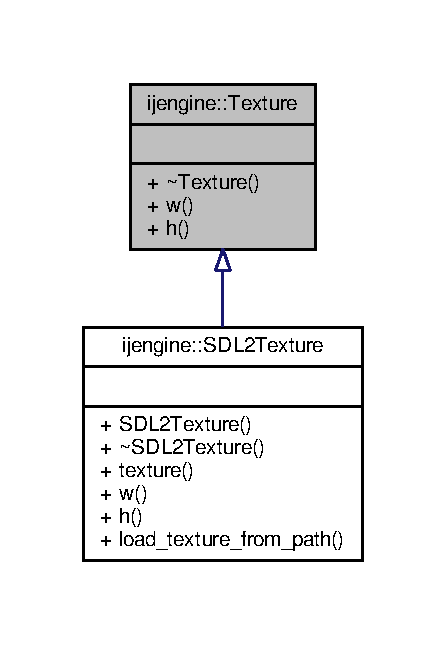
\includegraphics[width=214pt]{classijengine_1_1Texture__inherit__graph}
\end{center}
\end{figure}


Collaboration diagram for ijengine\-:\-:Texture\-:\nopagebreak
\begin{figure}[H]
\begin{center}
\leavevmode
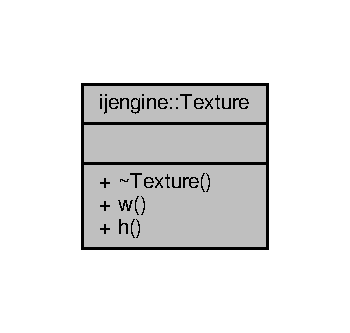
\includegraphics[width=168pt]{classijengine_1_1Texture__coll__graph}
\end{center}
\end{figure}
\subsection*{Public Member Functions}
\begin{DoxyCompactItemize}
\item 
virtual \hyperlink{classijengine_1_1Texture_a26cfdb0fc73d02c6ffc9de4ef2786505}{$\sim$\-Texture} ()=default
\item 
virtual int \hyperlink{classijengine_1_1Texture_a8de34c2971f12e08d49c5f51d8236178}{w} () const =0
\item 
virtual int \hyperlink{classijengine_1_1Texture_a9ffe6059a07f4f20251578d9d9f9334c}{h} () const =0
\end{DoxyCompactItemize}


\subsection{Constructor \& Destructor Documentation}
\hypertarget{classijengine_1_1Texture_a26cfdb0fc73d02c6ffc9de4ef2786505}{\index{ijengine\-::\-Texture@{ijengine\-::\-Texture}!$\sim$\-Texture@{$\sim$\-Texture}}
\index{$\sim$\-Texture@{$\sim$\-Texture}!ijengine::Texture@{ijengine\-::\-Texture}}
\subsubsection[{$\sim$\-Texture}]{\setlength{\rightskip}{0pt plus 5cm}virtual ijengine\-::\-Texture\-::$\sim$\-Texture (
\begin{DoxyParamCaption}
{}
\end{DoxyParamCaption}
)\hspace{0.3cm}{\ttfamily [virtual]}, {\ttfamily [default]}}}\label{classijengine_1_1Texture_a26cfdb0fc73d02c6ffc9de4ef2786505}


\subsection{Member Function Documentation}
\hypertarget{classijengine_1_1Texture_a9ffe6059a07f4f20251578d9d9f9334c}{\index{ijengine\-::\-Texture@{ijengine\-::\-Texture}!h@{h}}
\index{h@{h}!ijengine::Texture@{ijengine\-::\-Texture}}
\subsubsection[{h}]{\setlength{\rightskip}{0pt plus 5cm}virtual int ijengine\-::\-Texture\-::h (
\begin{DoxyParamCaption}
{}
\end{DoxyParamCaption}
) const\hspace{0.3cm}{\ttfamily [pure virtual]}}}\label{classijengine_1_1Texture_a9ffe6059a07f4f20251578d9d9f9334c}


Implemented in \hyperlink{classijengine_1_1SDL2Texture_a5202ccb0ca2cd152fd3597b45235556e}{ijengine\-::\-S\-D\-L2\-Texture}.

\hypertarget{classijengine_1_1Texture_a8de34c2971f12e08d49c5f51d8236178}{\index{ijengine\-::\-Texture@{ijengine\-::\-Texture}!w@{w}}
\index{w@{w}!ijengine::Texture@{ijengine\-::\-Texture}}
\subsubsection[{w}]{\setlength{\rightskip}{0pt plus 5cm}virtual int ijengine\-::\-Texture\-::w (
\begin{DoxyParamCaption}
{}
\end{DoxyParamCaption}
) const\hspace{0.3cm}{\ttfamily [pure virtual]}}}\label{classijengine_1_1Texture_a8de34c2971f12e08d49c5f51d8236178}


Implemented in \hyperlink{classijengine_1_1SDL2Texture_a94b43ffad7f1ea5ac74165e59085ffce}{ijengine\-::\-S\-D\-L2\-Texture}.



The documentation for this class was generated from the following file\-:\begin{DoxyCompactItemize}
\item 
/home/carla/git/ijengine-\/\-I\-C\-G\-\_\-\-G\-L/include/\hyperlink{texture_8h}{texture.\-h}\end{DoxyCompactItemize}

\hypertarget{structijengine_1_1Vector3f}{\section{ijengine\-:\-:Vector3f Struct Reference}
\label{structijengine_1_1Vector3f}\index{ijengine\-::\-Vector3f@{ijengine\-::\-Vector3f}}
}


{\ttfamily \#include $<$vertexformat.\-h$>$}



Collaboration diagram for ijengine\-:\-:Vector3f\-:\nopagebreak
\begin{figure}[H]
\begin{center}
\leavevmode
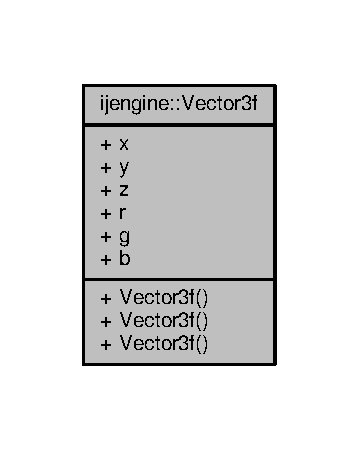
\includegraphics[width=172pt]{structijengine_1_1Vector3f__coll__graph}
\end{center}
\end{figure}
\subsection*{Public Member Functions}
\begin{DoxyCompactItemize}
\item 
\hyperlink{structijengine_1_1Vector3f_a64ff073054db67b57009602892f3c8fa}{Vector3f} ()
\item 
\hyperlink{structijengine_1_1Vector3f_a50975b389d1a92cbb68bbf82864ce929}{Vector3f} (float \-\_\-x, float \-\_\-y, float \-\_\-z)
\item 
\hyperlink{structijengine_1_1Vector3f_a326dfdae474265681ec0a6d85fa05e20}{Vector3f} (float \-\_\-x, float \-\_\-y, float \-\_\-z, float \-\_\-r, float \-\_\-g, float \-\_\-b)
\end{DoxyCompactItemize}
\subsection*{Public Attributes}
\begin{DoxyCompactItemize}
\item 
float \hyperlink{structijengine_1_1Vector3f_a62f586236d9e15cd6c95d354138f4362}{x}
\item 
float \hyperlink{structijengine_1_1Vector3f_a92ab51702f08a8dd02f7b5eecac5d16f}{y}
\item 
float \hyperlink{structijengine_1_1Vector3f_a79837bed7b540c2f5191ccb841e97b32}{z}
\item 
float \hyperlink{structijengine_1_1Vector3f_a0e7ca8f82170904af1d5132671e744b6}{r}
\item 
float \hyperlink{structijengine_1_1Vector3f_aed60781da1bd07f723e3afe4136bc0ce}{g}
\item 
float \hyperlink{structijengine_1_1Vector3f_a7e2ca78b9123dbfc1f2062e2bb8cb080}{b}
\end{DoxyCompactItemize}


\subsection{Constructor \& Destructor Documentation}
\hypertarget{structijengine_1_1Vector3f_a64ff073054db67b57009602892f3c8fa}{\index{ijengine\-::\-Vector3f@{ijengine\-::\-Vector3f}!Vector3f@{Vector3f}}
\index{Vector3f@{Vector3f}!ijengine::Vector3f@{ijengine\-::\-Vector3f}}
\subsubsection[{Vector3f}]{\setlength{\rightskip}{0pt plus 5cm}ijengine\-::\-Vector3f\-::\-Vector3f (
\begin{DoxyParamCaption}
{}
\end{DoxyParamCaption}
)\hspace{0.3cm}{\ttfamily [inline]}}}\label{structijengine_1_1Vector3f_a64ff073054db67b57009602892f3c8fa}
\hypertarget{structijengine_1_1Vector3f_a50975b389d1a92cbb68bbf82864ce929}{\index{ijengine\-::\-Vector3f@{ijengine\-::\-Vector3f}!Vector3f@{Vector3f}}
\index{Vector3f@{Vector3f}!ijengine::Vector3f@{ijengine\-::\-Vector3f}}
\subsubsection[{Vector3f}]{\setlength{\rightskip}{0pt plus 5cm}ijengine\-::\-Vector3f\-::\-Vector3f (
\begin{DoxyParamCaption}
\item[{float}]{\-\_\-x, }
\item[{float}]{\-\_\-y, }
\item[{float}]{\-\_\-z}
\end{DoxyParamCaption}
)\hspace{0.3cm}{\ttfamily [inline]}}}\label{structijengine_1_1Vector3f_a50975b389d1a92cbb68bbf82864ce929}
\hypertarget{structijengine_1_1Vector3f_a326dfdae474265681ec0a6d85fa05e20}{\index{ijengine\-::\-Vector3f@{ijengine\-::\-Vector3f}!Vector3f@{Vector3f}}
\index{Vector3f@{Vector3f}!ijengine::Vector3f@{ijengine\-::\-Vector3f}}
\subsubsection[{Vector3f}]{\setlength{\rightskip}{0pt plus 5cm}ijengine\-::\-Vector3f\-::\-Vector3f (
\begin{DoxyParamCaption}
\item[{float}]{\-\_\-x, }
\item[{float}]{\-\_\-y, }
\item[{float}]{\-\_\-z, }
\item[{float}]{\-\_\-r, }
\item[{float}]{\-\_\-g, }
\item[{float}]{\-\_\-b}
\end{DoxyParamCaption}
)\hspace{0.3cm}{\ttfamily [inline]}}}\label{structijengine_1_1Vector3f_a326dfdae474265681ec0a6d85fa05e20}


\subsection{Member Data Documentation}
\hypertarget{structijengine_1_1Vector3f_a7e2ca78b9123dbfc1f2062e2bb8cb080}{\index{ijengine\-::\-Vector3f@{ijengine\-::\-Vector3f}!b@{b}}
\index{b@{b}!ijengine::Vector3f@{ijengine\-::\-Vector3f}}
\subsubsection[{b}]{\setlength{\rightskip}{0pt plus 5cm}float ijengine\-::\-Vector3f\-::b}}\label{structijengine_1_1Vector3f_a7e2ca78b9123dbfc1f2062e2bb8cb080}
\hypertarget{structijengine_1_1Vector3f_aed60781da1bd07f723e3afe4136bc0ce}{\index{ijengine\-::\-Vector3f@{ijengine\-::\-Vector3f}!g@{g}}
\index{g@{g}!ijengine::Vector3f@{ijengine\-::\-Vector3f}}
\subsubsection[{g}]{\setlength{\rightskip}{0pt plus 5cm}float ijengine\-::\-Vector3f\-::g}}\label{structijengine_1_1Vector3f_aed60781da1bd07f723e3afe4136bc0ce}
\hypertarget{structijengine_1_1Vector3f_a0e7ca8f82170904af1d5132671e744b6}{\index{ijengine\-::\-Vector3f@{ijengine\-::\-Vector3f}!r@{r}}
\index{r@{r}!ijengine::Vector3f@{ijengine\-::\-Vector3f}}
\subsubsection[{r}]{\setlength{\rightskip}{0pt plus 5cm}float ijengine\-::\-Vector3f\-::r}}\label{structijengine_1_1Vector3f_a0e7ca8f82170904af1d5132671e744b6}
\hypertarget{structijengine_1_1Vector3f_a62f586236d9e15cd6c95d354138f4362}{\index{ijengine\-::\-Vector3f@{ijengine\-::\-Vector3f}!x@{x}}
\index{x@{x}!ijengine::Vector3f@{ijengine\-::\-Vector3f}}
\subsubsection[{x}]{\setlength{\rightskip}{0pt plus 5cm}float ijengine\-::\-Vector3f\-::x}}\label{structijengine_1_1Vector3f_a62f586236d9e15cd6c95d354138f4362}
\hypertarget{structijengine_1_1Vector3f_a92ab51702f08a8dd02f7b5eecac5d16f}{\index{ijengine\-::\-Vector3f@{ijengine\-::\-Vector3f}!y@{y}}
\index{y@{y}!ijengine::Vector3f@{ijengine\-::\-Vector3f}}
\subsubsection[{y}]{\setlength{\rightskip}{0pt plus 5cm}float ijengine\-::\-Vector3f\-::y}}\label{structijengine_1_1Vector3f_a92ab51702f08a8dd02f7b5eecac5d16f}
\hypertarget{structijengine_1_1Vector3f_a79837bed7b540c2f5191ccb841e97b32}{\index{ijengine\-::\-Vector3f@{ijengine\-::\-Vector3f}!z@{z}}
\index{z@{z}!ijengine::Vector3f@{ijengine\-::\-Vector3f}}
\subsubsection[{z}]{\setlength{\rightskip}{0pt plus 5cm}float ijengine\-::\-Vector3f\-::z}}\label{structijengine_1_1Vector3f_a79837bed7b540c2f5191ccb841e97b32}


The documentation for this struct was generated from the following file\-:\begin{DoxyCompactItemize}
\item 
/home/carla/git/ijengine-\/\-I\-C\-G\-\_\-\-G\-L/include/\hyperlink{vertexformat_8h}{vertexformat.\-h}\end{DoxyCompactItemize}

\hypertarget{classijengine_1_1Video}{\section{ijengine\-:\-:Video Class Reference}
\label{classijengine_1_1Video}\index{ijengine\-::\-Video@{ijengine\-::\-Video}}
}


{\ttfamily \#include $<$video.\-h$>$}



Inheritance diagram for ijengine\-:\-:Video\-:\nopagebreak
\begin{figure}[H]
\begin{center}
\leavevmode
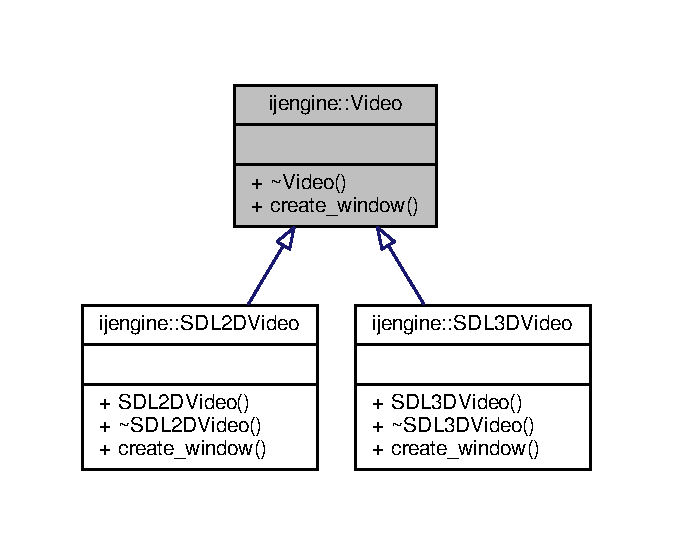
\includegraphics[width=323pt]{classijengine_1_1Video__inherit__graph}
\end{center}
\end{figure}


Collaboration diagram for ijengine\-:\-:Video\-:\nopagebreak
\begin{figure}[H]
\begin{center}
\leavevmode
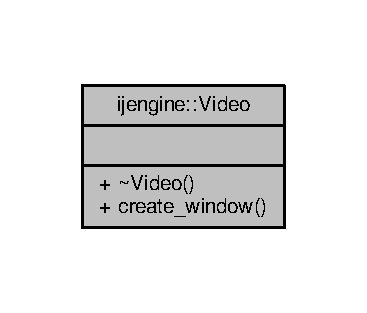
\includegraphics[width=176pt]{classijengine_1_1Video__coll__graph}
\end{center}
\end{figure}
\subsection*{Public Member Functions}
\begin{DoxyCompactItemize}
\item 
virtual \hyperlink{classijengine_1_1Video_abb66793ac4b5c66ac5f1a1755e4850bf}{$\sim$\-Video} ()=default
\item 
virtual \hyperlink{classijengine_1_1Window}{Window} $\ast$ \hyperlink{classijengine_1_1Video_a21c552c463b2a7466394c2b6e7e1ca99}{create\-\_\-window} (int w, int h)=0
\end{DoxyCompactItemize}


\subsection{Constructor \& Destructor Documentation}
\hypertarget{classijengine_1_1Video_abb66793ac4b5c66ac5f1a1755e4850bf}{\index{ijengine\-::\-Video@{ijengine\-::\-Video}!$\sim$\-Video@{$\sim$\-Video}}
\index{$\sim$\-Video@{$\sim$\-Video}!ijengine::Video@{ijengine\-::\-Video}}
\subsubsection[{$\sim$\-Video}]{\setlength{\rightskip}{0pt plus 5cm}virtual ijengine\-::\-Video\-::$\sim$\-Video (
\begin{DoxyParamCaption}
{}
\end{DoxyParamCaption}
)\hspace{0.3cm}{\ttfamily [virtual]}, {\ttfamily [default]}}}\label{classijengine_1_1Video_abb66793ac4b5c66ac5f1a1755e4850bf}


\subsection{Member Function Documentation}
\hypertarget{classijengine_1_1Video_a21c552c463b2a7466394c2b6e7e1ca99}{\index{ijengine\-::\-Video@{ijengine\-::\-Video}!create\-\_\-window@{create\-\_\-window}}
\index{create\-\_\-window@{create\-\_\-window}!ijengine::Video@{ijengine\-::\-Video}}
\subsubsection[{create\-\_\-window}]{\setlength{\rightskip}{0pt plus 5cm}virtual {\bf Window}$\ast$ ijengine\-::\-Video\-::create\-\_\-window (
\begin{DoxyParamCaption}
\item[{int}]{w, }
\item[{int}]{h}
\end{DoxyParamCaption}
)\hspace{0.3cm}{\ttfamily [pure virtual]}}}\label{classijengine_1_1Video_a21c552c463b2a7466394c2b6e7e1ca99}


Implemented in \hyperlink{classijengine_1_1SDL2DVideo_a560fb324f6dcc18936901d4c91fa8e89}{ijengine\-::\-S\-D\-L2\-D\-Video}, and \hyperlink{classijengine_1_1SDL3DVideo_a91129138ce05c6d1f453f7cc854dba3f}{ijengine\-::\-S\-D\-L3\-D\-Video}.



The documentation for this class was generated from the following file\-:\begin{DoxyCompactItemize}
\item 
/home/carla/git/ijengine-\/\-I\-C\-G\-\_\-\-G\-L/include/\hyperlink{video_8h}{video.\-h}\end{DoxyCompactItemize}

\hypertarget{classijengine_1_1Window}{\section{ijengine\-:\-:Window Class Reference}
\label{classijengine_1_1Window}\index{ijengine\-::\-Window@{ijengine\-::\-Window}}
}


{\ttfamily \#include $<$window.\-h$>$}



Inheritance diagram for ijengine\-:\-:Window\-:\nopagebreak
\begin{figure}[H]
\begin{center}
\leavevmode
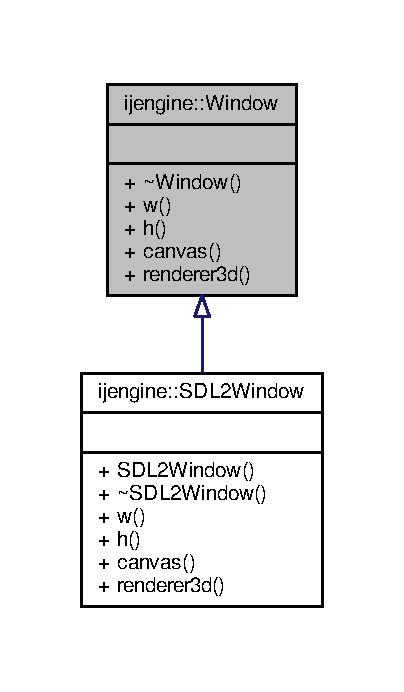
\includegraphics[width=194pt]{classijengine_1_1Window__inherit__graph}
\end{center}
\end{figure}


Collaboration diagram for ijengine\-:\-:Window\-:\nopagebreak
\begin{figure}[H]
\begin{center}
\leavevmode
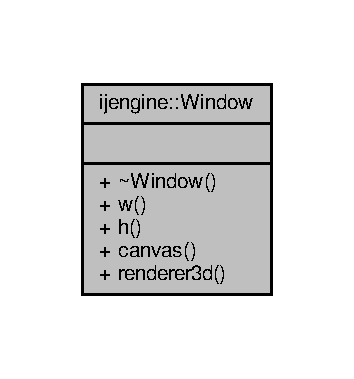
\includegraphics[width=170pt]{classijengine_1_1Window__coll__graph}
\end{center}
\end{figure}
\subsection*{Public Member Functions}
\begin{DoxyCompactItemize}
\item 
virtual \hyperlink{classijengine_1_1Window_a5c7cf239d20dcf1a379f09e6ba6dcecf}{$\sim$\-Window} ()=default
\item 
virtual int \hyperlink{classijengine_1_1Window_a0481e6a3e12e4455cbc7205bcb7507de}{w} () const =0
\item 
virtual int \hyperlink{classijengine_1_1Window_a1f77cd9da190853e8721a2f18bc2ffba}{h} () const =0
\item 
virtual \hyperlink{classijengine_1_1Canvas}{Canvas} $\ast$ \hyperlink{classijengine_1_1Window_ad09bf41db3b3c65bdaaebb1986eee285}{canvas} () const =0
\item 
virtual \hyperlink{classijengine_1_1Renderer3d}{Renderer3d} $\ast$ \hyperlink{classijengine_1_1Window_aaa4026b334e10318ec1ea92bf62a4a90}{renderer3d} () const =0
\end{DoxyCompactItemize}


\subsection{Constructor \& Destructor Documentation}
\hypertarget{classijengine_1_1Window_a5c7cf239d20dcf1a379f09e6ba6dcecf}{\index{ijengine\-::\-Window@{ijengine\-::\-Window}!$\sim$\-Window@{$\sim$\-Window}}
\index{$\sim$\-Window@{$\sim$\-Window}!ijengine::Window@{ijengine\-::\-Window}}
\subsubsection[{$\sim$\-Window}]{\setlength{\rightskip}{0pt plus 5cm}virtual ijengine\-::\-Window\-::$\sim$\-Window (
\begin{DoxyParamCaption}
{}
\end{DoxyParamCaption}
)\hspace{0.3cm}{\ttfamily [virtual]}, {\ttfamily [default]}}}\label{classijengine_1_1Window_a5c7cf239d20dcf1a379f09e6ba6dcecf}


\subsection{Member Function Documentation}
\hypertarget{classijengine_1_1Window_ad09bf41db3b3c65bdaaebb1986eee285}{\index{ijengine\-::\-Window@{ijengine\-::\-Window}!canvas@{canvas}}
\index{canvas@{canvas}!ijengine::Window@{ijengine\-::\-Window}}
\subsubsection[{canvas}]{\setlength{\rightskip}{0pt plus 5cm}virtual {\bf Canvas}$\ast$ ijengine\-::\-Window\-::canvas (
\begin{DoxyParamCaption}
{}
\end{DoxyParamCaption}
) const\hspace{0.3cm}{\ttfamily [pure virtual]}}}\label{classijengine_1_1Window_ad09bf41db3b3c65bdaaebb1986eee285}


Implemented in \hyperlink{classijengine_1_1SDL2Window_a67813fe0b83700d046a4b84112b9ceb3}{ijengine\-::\-S\-D\-L2\-Window}.

\hypertarget{classijengine_1_1Window_a1f77cd9da190853e8721a2f18bc2ffba}{\index{ijengine\-::\-Window@{ijengine\-::\-Window}!h@{h}}
\index{h@{h}!ijengine::Window@{ijengine\-::\-Window}}
\subsubsection[{h}]{\setlength{\rightskip}{0pt plus 5cm}virtual int ijengine\-::\-Window\-::h (
\begin{DoxyParamCaption}
{}
\end{DoxyParamCaption}
) const\hspace{0.3cm}{\ttfamily [pure virtual]}}}\label{classijengine_1_1Window_a1f77cd9da190853e8721a2f18bc2ffba}


Implemented in \hyperlink{classijengine_1_1SDL2Window_a22bfc90a19791ec62bee093b573a1317}{ijengine\-::\-S\-D\-L2\-Window}.

\hypertarget{classijengine_1_1Window_aaa4026b334e10318ec1ea92bf62a4a90}{\index{ijengine\-::\-Window@{ijengine\-::\-Window}!renderer3d@{renderer3d}}
\index{renderer3d@{renderer3d}!ijengine::Window@{ijengine\-::\-Window}}
\subsubsection[{renderer3d}]{\setlength{\rightskip}{0pt plus 5cm}virtual {\bf Renderer3d}$\ast$ ijengine\-::\-Window\-::renderer3d (
\begin{DoxyParamCaption}
{}
\end{DoxyParamCaption}
) const\hspace{0.3cm}{\ttfamily [pure virtual]}}}\label{classijengine_1_1Window_aaa4026b334e10318ec1ea92bf62a4a90}


Implemented in \hyperlink{classijengine_1_1SDL2Window_aa35b142bef03f2fd5fc17382bfef39f1}{ijengine\-::\-S\-D\-L2\-Window}.

\hypertarget{classijengine_1_1Window_a0481e6a3e12e4455cbc7205bcb7507de}{\index{ijengine\-::\-Window@{ijengine\-::\-Window}!w@{w}}
\index{w@{w}!ijengine::Window@{ijengine\-::\-Window}}
\subsubsection[{w}]{\setlength{\rightskip}{0pt plus 5cm}virtual int ijengine\-::\-Window\-::w (
\begin{DoxyParamCaption}
{}
\end{DoxyParamCaption}
) const\hspace{0.3cm}{\ttfamily [pure virtual]}}}\label{classijengine_1_1Window_a0481e6a3e12e4455cbc7205bcb7507de}


Implemented in \hyperlink{classijengine_1_1SDL2Window_a9ee858781f682de6e1f4e07e0e005d52}{ijengine\-::\-S\-D\-L2\-Window}.



The documentation for this class was generated from the following file\-:\begin{DoxyCompactItemize}
\item 
/home/carla/git/ijengine-\/\-I\-C\-G\-\_\-\-G\-L/include/\hyperlink{window_8h}{window.\-h}\end{DoxyCompactItemize}

\chapter{File Documentation}
\hypertarget{canvas_8h}{\section{/home/carla/git/ijengine-\/\-I\-C\-G\-\_\-\-G\-L/include/canvas.h File Reference}
\label{canvas_8h}\index{/home/carla/git/ijengine-\/\-I\-C\-G\-\_\-\-G\-L/include/canvas.\-h@{/home/carla/git/ijengine-\/\-I\-C\-G\-\_\-\-G\-L/include/canvas.\-h}}
}
This graph shows which files directly or indirectly include this file\-:\nopagebreak
\begin{figure}[H]
\begin{center}
\leavevmode
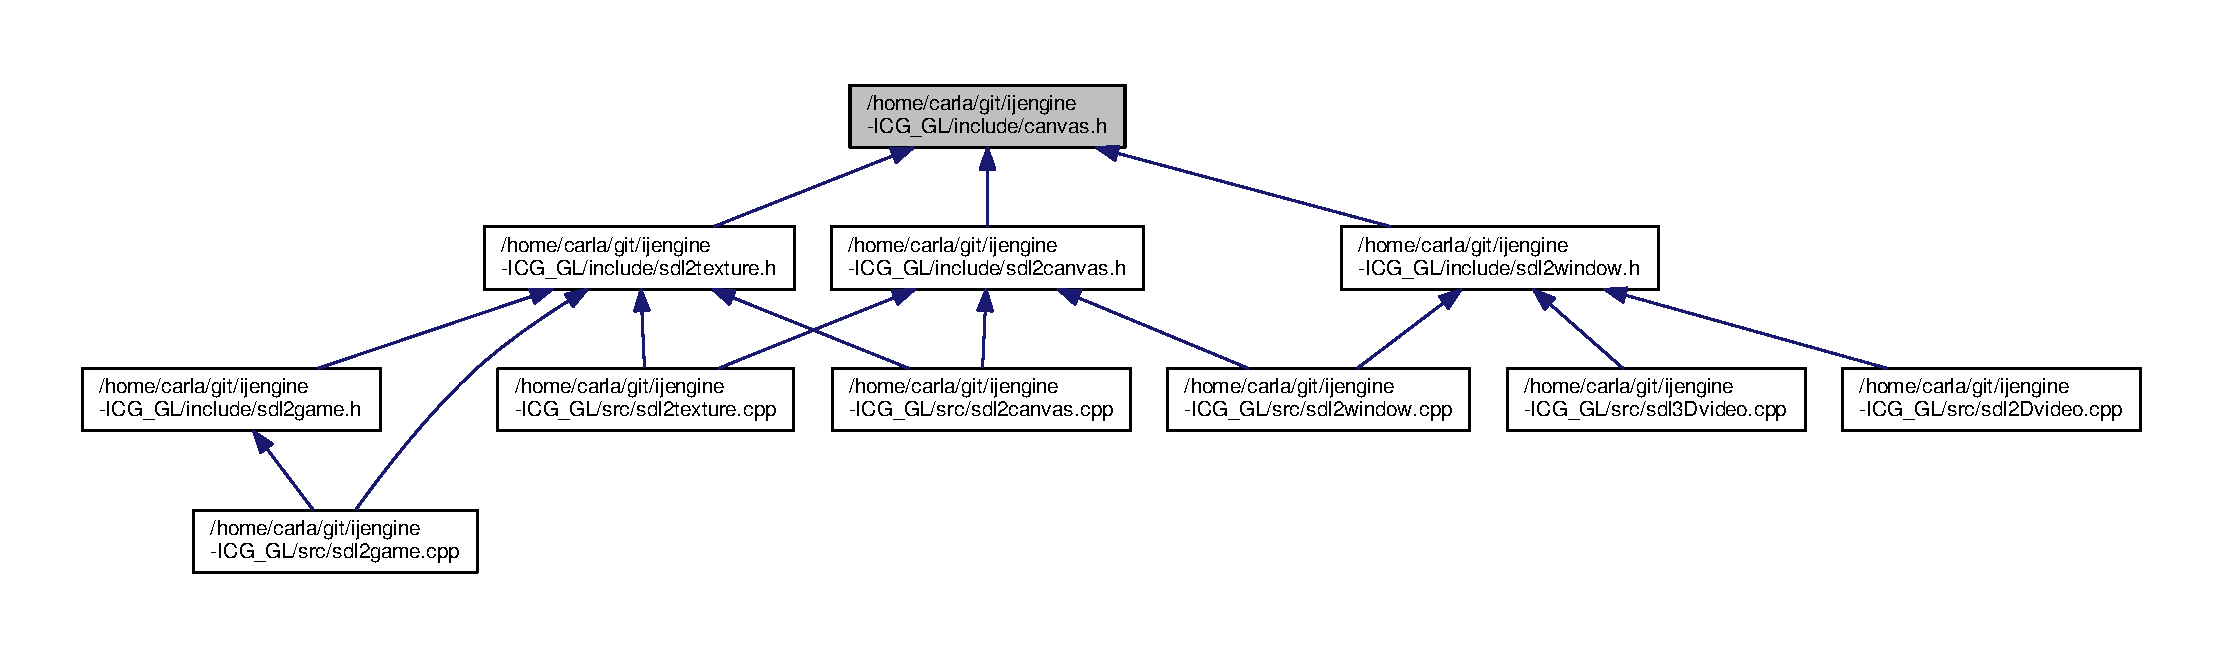
\includegraphics[width=350pt]{canvas_8h__dep__incl}
\end{center}
\end{figure}
\subsection*{Classes}
\begin{DoxyCompactItemize}
\item 
class \hyperlink{classijengine_1_1Canvas}{ijengine\-::\-Canvas}
\end{DoxyCompactItemize}
\subsection*{Namespaces}
\begin{DoxyCompactItemize}
\item 
\hyperlink{namespaceijengine}{ijengine}
\end{DoxyCompactItemize}

\hypertarget{contextinfo_8h}{\section{/home/carla/git/ijengine-\/\-I\-C\-G\-\_\-\-G\-L/include/contextinfo.h File Reference}
\label{contextinfo_8h}\index{/home/carla/git/ijengine-\/\-I\-C\-G\-\_\-\-G\-L/include/contextinfo.\-h@{/home/carla/git/ijengine-\/\-I\-C\-G\-\_\-\-G\-L/include/contextinfo.\-h}}
}
\subsection*{Classes}
\begin{DoxyCompactItemize}
\item 
struct \hyperlink{structijengine_1_1ContextInfo}{ijengine\-::\-Context\-Info}
\end{DoxyCompactItemize}
\subsection*{Namespaces}
\begin{DoxyCompactItemize}
\item 
\hyperlink{namespaceijengine}{ijengine}
\end{DoxyCompactItemize}

\hypertarget{framebufferinfo_8h}{\section{/home/carla/git/ijengine-\/\-I\-C\-G\-\_\-\-G\-L/include/framebufferinfo.h File Reference}
\label{framebufferinfo_8h}\index{/home/carla/git/ijengine-\/\-I\-C\-G\-\_\-\-G\-L/include/framebufferinfo.\-h@{/home/carla/git/ijengine-\/\-I\-C\-G\-\_\-\-G\-L/include/framebufferinfo.\-h}}
}
{\ttfamily \#include $<$S\-D\-L2/\-S\-D\-L.\-h$>$}\\*
Include dependency graph for framebufferinfo.\-h\-:\nopagebreak
\begin{figure}[H]
\begin{center}
\leavevmode
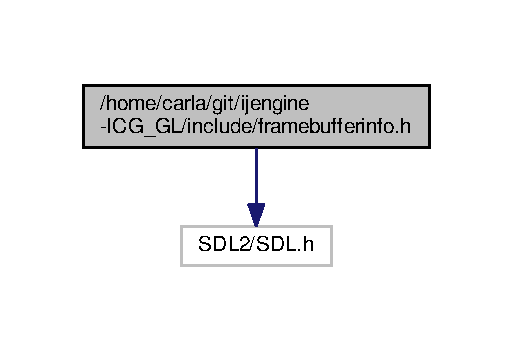
\includegraphics[width=246pt]{framebufferinfo_8h__incl}
\end{center}
\end{figure}
\subsection*{Classes}
\begin{DoxyCompactItemize}
\item 
struct \hyperlink{structijengine_1_1FramebufferInfo}{ijengine\-::\-Framebuffer\-Info}
\end{DoxyCompactItemize}
\subsection*{Namespaces}
\begin{DoxyCompactItemize}
\item 
\hyperlink{namespaceijengine}{ijengine}
\end{DoxyCompactItemize}

\hypertarget{game_8h}{\section{/home/carla/git/ijengine-\/\-I\-C\-G\-\_\-\-G\-L/include/game.h File Reference}
\label{game_8h}\index{/home/carla/git/ijengine-\/\-I\-C\-G\-\_\-\-G\-L/include/game.\-h@{/home/carla/git/ijengine-\/\-I\-C\-G\-\_\-\-G\-L/include/game.\-h}}
}
This graph shows which files directly or indirectly include this file\-:\nopagebreak
\begin{figure}[H]
\begin{center}
\leavevmode
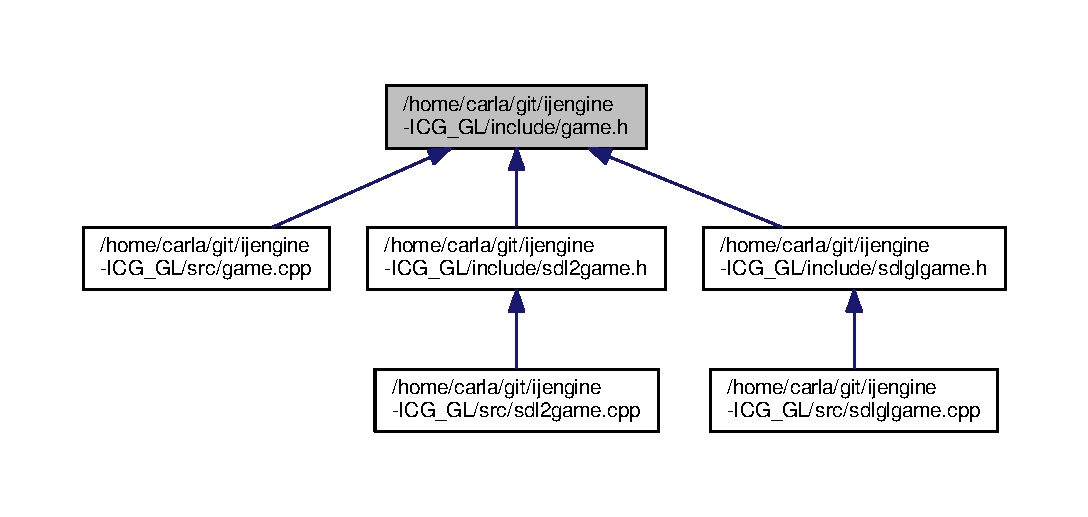
\includegraphics[width=350pt]{game_8h__dep__incl}
\end{center}
\end{figure}
\subsection*{Classes}
\begin{DoxyCompactItemize}
\item 
class \hyperlink{classijengine_1_1Game}{ijengine\-::\-Game}
\end{DoxyCompactItemize}
\subsection*{Namespaces}
\begin{DoxyCompactItemize}
\item 
\hyperlink{namespaceijengine}{ijengine}
\end{DoxyCompactItemize}

\hypertarget{gamemodels_8h}{\section{/home/carla/git/ijengine-\/\-I\-C\-G\-\_\-\-G\-L/include/gamemodels.h File Reference}
\label{gamemodels_8h}\index{/home/carla/git/ijengine-\/\-I\-C\-G\-\_\-\-G\-L/include/gamemodels.\-h@{/home/carla/git/ijengine-\/\-I\-C\-G\-\_\-\-G\-L/include/gamemodels.\-h}}
}
{\ttfamily \#include $<$vector$>$}\\*
{\ttfamily \#include $<$map$>$}\\*
Include dependency graph for gamemodels.\-h\-:\nopagebreak
\begin{figure}[H]
\begin{center}
\leavevmode
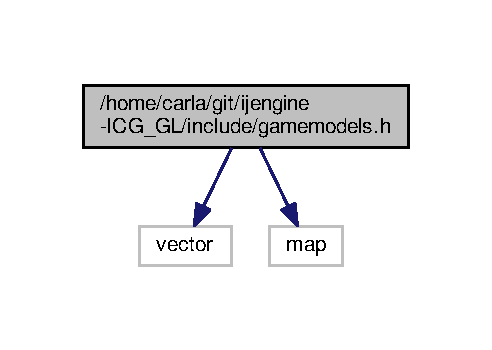
\includegraphics[width=236pt]{gamemodels_8h__incl}
\end{center}
\end{figure}
\subsection*{Classes}
\begin{DoxyCompactItemize}
\item 
class \hyperlink{structijengine_1_1Model}{ijengine\-::\-Model}
\item 
class \hyperlink{classijengine_1_1GameModels}{ijengine\-::\-Game\-Models}
\end{DoxyCompactItemize}
\subsection*{Namespaces}
\begin{DoxyCompactItemize}
\item 
\hyperlink{namespaceijengine}{ijengine}
\end{DoxyCompactItemize}

\hypertarget{glrenderer3d_8h}{\section{/home/carla/git/ijengine-\/\-I\-C\-G\-\_\-\-G\-L/include/glrenderer3d.h File Reference}
\label{glrenderer3d_8h}\index{/home/carla/git/ijengine-\/\-I\-C\-G\-\_\-\-G\-L/include/glrenderer3d.\-h@{/home/carla/git/ijengine-\/\-I\-C\-G\-\_\-\-G\-L/include/glrenderer3d.\-h}}
}
{\ttfamily \#include $<$G\-L/glew.\-h$>$}\\*
{\ttfamily \#include $<$G\-L/gl.\-h$>$}\\*
{\ttfamily \#include $<$G\-L/glu.\-h$>$}\\*
{\ttfamily \#include $<$S\-D\-L2/\-S\-D\-L.\-h$>$}\\*
{\ttfamily \#include \char`\"{}renderer3d.\-h\char`\"{}}\\*
Include dependency graph for glrenderer3d.\-h\-:\nopagebreak
\begin{figure}[H]
\begin{center}
\leavevmode
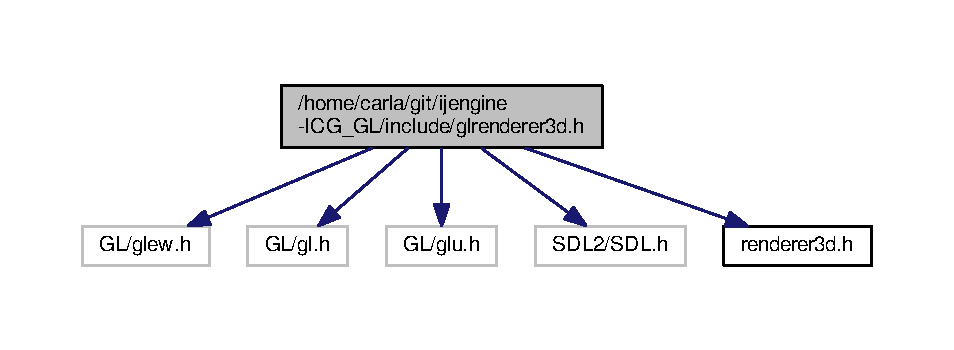
\includegraphics[width=350pt]{glrenderer3d_8h__incl}
\end{center}
\end{figure}
This graph shows which files directly or indirectly include this file\-:\nopagebreak
\begin{figure}[H]
\begin{center}
\leavevmode
\includegraphics[width=350pt]{glrenderer3d_8h__dep__incl}
\end{center}
\end{figure}
\subsection*{Classes}
\begin{DoxyCompactItemize}
\item 
class \hyperlink{classGLrenderer3d}{G\-Lrenderer3d}
\end{DoxyCompactItemize}

\hypertarget{Igameobject_8h}{\section{/home/carla/git/ijengine-\/\-I\-C\-G\-\_\-\-G\-L/include/\-Igameobject.h File Reference}
\label{Igameobject_8h}\index{/home/carla/git/ijengine-\/\-I\-C\-G\-\_\-\-G\-L/include/\-Igameobject.\-h@{/home/carla/git/ijengine-\/\-I\-C\-G\-\_\-\-G\-L/include/\-Igameobject.\-h}}
}
{\ttfamily \#include $<$vector$>$}\\*
{\ttfamily \#include $<$iostream$>$}\\*
{\ttfamily \#include \char`\"{}G\-L/glew.\-h\char`\"{}}\\*
Include dependency graph for Igameobject.\-h\-:\nopagebreak
\begin{figure}[H]
\begin{center}
\leavevmode
\includegraphics[width=275pt]{Igameobject_8h__incl}
\end{center}
\end{figure}
\subsection*{Namespaces}
\begin{DoxyCompactItemize}
\item 
\hyperlink{namespaceijengine}{ijengine}
\end{DoxyCompactItemize}

\hypertarget{libgl_8h}{\section{/home/carla/git/ijengine-\/\-I\-C\-G\-\_\-\-G\-L/include/libgl.h File Reference}
\label{libgl_8h}\index{/home/carla/git/ijengine-\/\-I\-C\-G\-\_\-\-G\-L/include/libgl.\-h@{/home/carla/git/ijengine-\/\-I\-C\-G\-\_\-\-G\-L/include/libgl.\-h}}
}
{\ttfamily \#include \char`\"{}libs.\-h\char`\"{}}\\*
Include dependency graph for libgl.\-h\-:\nopagebreak
\begin{figure}[H]
\begin{center}
\leavevmode
\includegraphics[width=198pt]{libgl_8h__incl}
\end{center}
\end{figure}
This graph shows which files directly or indirectly include this file\-:\nopagebreak
\begin{figure}[H]
\begin{center}
\leavevmode
\includegraphics[width=350pt]{libgl_8h__dep__incl}
\end{center}
\end{figure}
\subsection*{Classes}
\begin{DoxyCompactItemize}
\item 
class \hyperlink{classijengine_1_1LibGL}{ijengine\-::\-Lib\-G\-L}
\end{DoxyCompactItemize}
\subsection*{Namespaces}
\begin{DoxyCompactItemize}
\item 
\hyperlink{namespaceijengine}{ijengine}
\end{DoxyCompactItemize}

\hypertarget{libs_8h}{\section{/home/carla/git/ijengine-\/\-I\-C\-G\-\_\-\-G\-L/include/libs.h File Reference}
\label{libs_8h}\index{/home/carla/git/ijengine-\/\-I\-C\-G\-\_\-\-G\-L/include/libs.\-h@{/home/carla/git/ijengine-\/\-I\-C\-G\-\_\-\-G\-L/include/libs.\-h}}
}
{\ttfamily \#include $<$string$>$}\\*
Include dependency graph for libs.\-h\-:\nopagebreak
\begin{figure}[H]
\begin{center}
\leavevmode
\includegraphics[width=196pt]{libs_8h__incl}
\end{center}
\end{figure}
This graph shows which files directly or indirectly include this file\-:\nopagebreak
\begin{figure}[H]
\begin{center}
\leavevmode
\includegraphics[width=350pt]{libs_8h__dep__incl}
\end{center}
\end{figure}
\subsection*{Classes}
\begin{DoxyCompactItemize}
\item 
class \hyperlink{classijengine_1_1Lib}{ijengine\-::\-Lib}
\end{DoxyCompactItemize}
\subsection*{Namespaces}
\begin{DoxyCompactItemize}
\item 
\hyperlink{namespaceijengine}{ijengine}
\end{DoxyCompactItemize}

\hypertarget{model_8h}{\section{/home/carla/git/ijengine-\/\-I\-C\-G\-\_\-\-G\-L/include/model.h File Reference}
\label{model_8h}\index{/home/carla/git/ijengine-\/\-I\-C\-G\-\_\-\-G\-L/include/model.\-h@{/home/carla/git/ijengine-\/\-I\-C\-G\-\_\-\-G\-L/include/model.\-h}}
}
{\ttfamily \#include $<$vector$>$}\\*
{\ttfamily \#include $<$iostream$>$}\\*
{\ttfamily \#include \char`\"{}G\-L/glew.\-h\char`\"{}}\\*
Include dependency graph for model.\-h\-:\nopagebreak
\begin{figure}[H]
\begin{center}
\leavevmode
\includegraphics[width=275pt]{model_8h__incl}
\end{center}
\end{figure}
\subsection*{Classes}
\begin{DoxyCompactItemize}
\item 
class \hyperlink{structijengine_1_1Model}{ijengine\-::\-Model}
\end{DoxyCompactItemize}
\subsection*{Namespaces}
\begin{DoxyCompactItemize}
\item 
\hyperlink{namespaceijengine}{ijengine}
\end{DoxyCompactItemize}

\hypertarget{renderer3d_8h}{\section{/home/carla/git/ijengine-\/\-I\-C\-G\-\_\-\-G\-L/include/renderer3d.h File Reference}
\label{renderer3d_8h}\index{/home/carla/git/ijengine-\/\-I\-C\-G\-\_\-\-G\-L/include/renderer3d.\-h@{/home/carla/git/ijengine-\/\-I\-C\-G\-\_\-\-G\-L/include/renderer3d.\-h}}
}
This graph shows which files directly or indirectly include this file\-:\nopagebreak
\begin{figure}[H]
\begin{center}
\leavevmode
\includegraphics[width=350pt]{renderer3d_8h__dep__incl}
\end{center}
\end{figure}
\subsection*{Classes}
\begin{DoxyCompactItemize}
\item 
class \hyperlink{classijengine_1_1Renderer3d}{ijengine\-::\-Renderer3d}
\end{DoxyCompactItemize}
\subsection*{Namespaces}
\begin{DoxyCompactItemize}
\item 
\hyperlink{namespaceijengine}{ijengine}
\end{DoxyCompactItemize}

\hypertarget{sdl2_8h}{\section{/home/carla/git/ijengine-\/\-I\-C\-G\-\_\-\-G\-L/include/sdl2.h File Reference}
\label{sdl2_8h}\index{/home/carla/git/ijengine-\/\-I\-C\-G\-\_\-\-G\-L/include/sdl2.\-h@{/home/carla/git/ijengine-\/\-I\-C\-G\-\_\-\-G\-L/include/sdl2.\-h}}
}
{\ttfamily \#include \char`\"{}libs.\-h\char`\"{}}\\*
Include dependency graph for sdl2.\-h\-:\nopagebreak
\begin{figure}[H]
\begin{center}
\leavevmode
\includegraphics[width=198pt]{sdl2_8h__incl}
\end{center}
\end{figure}
This graph shows which files directly or indirectly include this file\-:\nopagebreak
\begin{figure}[H]
\begin{center}
\leavevmode
\includegraphics[width=350pt]{sdl2_8h__dep__incl}
\end{center}
\end{figure}
\subsection*{Classes}
\begin{DoxyCompactItemize}
\item 
class \hyperlink{classijengine_1_1LibSDL2}{ijengine\-::\-Lib\-S\-D\-L2}
\end{DoxyCompactItemize}
\subsection*{Namespaces}
\begin{DoxyCompactItemize}
\item 
\hyperlink{namespaceijengine}{ijengine}
\end{DoxyCompactItemize}

\hypertarget{sdl2canvas_8h}{\section{/home/carla/git/ijengine-\/\-I\-C\-G\-\_\-\-G\-L/include/sdl2canvas.h File Reference}
\label{sdl2canvas_8h}\index{/home/carla/git/ijengine-\/\-I\-C\-G\-\_\-\-G\-L/include/sdl2canvas.\-h@{/home/carla/git/ijengine-\/\-I\-C\-G\-\_\-\-G\-L/include/sdl2canvas.\-h}}
}
{\ttfamily \#include $<$S\-D\-L2/\-S\-D\-L.\-h$>$}\\*
{\ttfamily \#include \char`\"{}canvas.\-h\char`\"{}}\\*
Include dependency graph for sdl2canvas.\-h\-:\nopagebreak
\begin{figure}[H]
\begin{center}
\leavevmode
\includegraphics[width=231pt]{sdl2canvas_8h__incl}
\end{center}
\end{figure}
This graph shows which files directly or indirectly include this file\-:\nopagebreak
\begin{figure}[H]
\begin{center}
\leavevmode
\includegraphics[width=350pt]{sdl2canvas_8h__dep__incl}
\end{center}
\end{figure}
\subsection*{Classes}
\begin{DoxyCompactItemize}
\item 
class \hyperlink{classijengine_1_1SDL2Canvas}{ijengine\-::\-S\-D\-L2\-Canvas}
\end{DoxyCompactItemize}
\subsection*{Namespaces}
\begin{DoxyCompactItemize}
\item 
\hyperlink{namespaceijengine}{ijengine}
\end{DoxyCompactItemize}

\hypertarget{sdl2Dvideo_8h}{\section{/home/carla/git/ijengine-\/\-I\-C\-G\-\_\-\-G\-L/include/sdl2\-Dvideo.h File Reference}
\label{sdl2Dvideo_8h}\index{/home/carla/git/ijengine-\/\-I\-C\-G\-\_\-\-G\-L/include/sdl2\-Dvideo.\-h@{/home/carla/git/ijengine-\/\-I\-C\-G\-\_\-\-G\-L/include/sdl2\-Dvideo.\-h}}
}
{\ttfamily \#include \char`\"{}video.\-h\char`\"{}}\\*
{\ttfamily \#include $<$S\-D\-L2/\-S\-D\-L.\-h$>$}\\*
Include dependency graph for sdl2\-Dvideo.\-h\-:\nopagebreak
\begin{figure}[H]
\begin{center}
\leavevmode
\includegraphics[width=229pt]{sdl2Dvideo_8h__incl}
\end{center}
\end{figure}
This graph shows which files directly or indirectly include this file\-:\nopagebreak
\begin{figure}[H]
\begin{center}
\leavevmode
\includegraphics[width=350pt]{sdl2Dvideo_8h__dep__incl}
\end{center}
\end{figure}
\subsection*{Classes}
\begin{DoxyCompactItemize}
\item 
class \hyperlink{classijengine_1_1SDL2DVideo}{ijengine\-::\-S\-D\-L2\-D\-Video}
\end{DoxyCompactItemize}
\subsection*{Namespaces}
\begin{DoxyCompactItemize}
\item 
\hyperlink{namespaceijengine}{ijengine}
\end{DoxyCompactItemize}

\hypertarget{sdl2game_8h}{\section{/home/carla/git/ijengine-\/\-I\-C\-G\-\_\-\-G\-L/include/sdl2game.h File Reference}
\label{sdl2game_8h}\index{/home/carla/git/ijengine-\/\-I\-C\-G\-\_\-\-G\-L/include/sdl2game.\-h@{/home/carla/git/ijengine-\/\-I\-C\-G\-\_\-\-G\-L/include/sdl2game.\-h}}
}
{\ttfamily \#include \char`\"{}game.\-h\char`\"{}}\\*
{\ttfamily \#include \char`\"{}sdl2.\-h\char`\"{}}\\*
{\ttfamily \#include \char`\"{}sdl2\-Dvideo.\-h\char`\"{}}\\*
{\ttfamily \#include \char`\"{}window.\-h\char`\"{}}\\*
{\ttfamily \#include \char`\"{}sdl2texture.\-h\char`\"{}}\\*
{\ttfamily \#include $<$memory$>$}\\*
Include dependency graph for sdl2game.\-h\-:\nopagebreak
\begin{figure}[H]
\begin{center}
\leavevmode
\includegraphics[width=350pt]{sdl2game_8h__incl}
\end{center}
\end{figure}
This graph shows which files directly or indirectly include this file\-:\nopagebreak
\begin{figure}[H]
\begin{center}
\leavevmode
\includegraphics[width=222pt]{sdl2game_8h__dep__incl}
\end{center}
\end{figure}
\subsection*{Classes}
\begin{DoxyCompactItemize}
\item 
class \hyperlink{classijengine_1_1SDL2Game}{ijengine\-::\-S\-D\-L2\-Game}
\end{DoxyCompactItemize}
\subsection*{Namespaces}
\begin{DoxyCompactItemize}
\item 
\hyperlink{namespaceijengine}{ijengine}
\end{DoxyCompactItemize}

\hypertarget{sdl2texture_8h}{\section{/home/carla/git/ijengine-\/\-I\-C\-G\-\_\-\-G\-L/include/sdl2texture.h File Reference}
\label{sdl2texture_8h}\index{/home/carla/git/ijengine-\/\-I\-C\-G\-\_\-\-G\-L/include/sdl2texture.\-h@{/home/carla/git/ijengine-\/\-I\-C\-G\-\_\-\-G\-L/include/sdl2texture.\-h}}
}
{\ttfamily \#include $<$S\-D\-L2/\-S\-D\-L.\-h$>$}\\*
{\ttfamily \#include $<$string$>$}\\*
{\ttfamily \#include \char`\"{}texture.\-h\char`\"{}}\\*
{\ttfamily \#include \char`\"{}canvas.\-h\char`\"{}}\\*
Include dependency graph for sdl2texture.\-h\-:\nopagebreak
\begin{figure}[H]
\begin{center}
\leavevmode
\includegraphics[width=350pt]{sdl2texture_8h__incl}
\end{center}
\end{figure}
This graph shows which files directly or indirectly include this file\-:\nopagebreak
\begin{figure}[H]
\begin{center}
\leavevmode
\includegraphics[width=350pt]{sdl2texture_8h__dep__incl}
\end{center}
\end{figure}
\subsection*{Classes}
\begin{DoxyCompactItemize}
\item 
class \hyperlink{classijengine_1_1SDL2Texture}{ijengine\-::\-S\-D\-L2\-Texture}
\end{DoxyCompactItemize}
\subsection*{Namespaces}
\begin{DoxyCompactItemize}
\item 
\hyperlink{namespaceijengine}{ijengine}
\end{DoxyCompactItemize}

\hypertarget{sdl2window_8h}{\section{/home/carla/git/ijengine-\/\-I\-C\-G\-\_\-\-G\-L/include/sdl2window.h File Reference}
\label{sdl2window_8h}\index{/home/carla/git/ijengine-\/\-I\-C\-G\-\_\-\-G\-L/include/sdl2window.\-h@{/home/carla/git/ijengine-\/\-I\-C\-G\-\_\-\-G\-L/include/sdl2window.\-h}}
}
{\ttfamily \#include \char`\"{}window.\-h\char`\"{}}\\*
{\ttfamily \#include $<$S\-D\-L2/\-S\-D\-L.\-h$>$}\\*
{\ttfamily \#include \char`\"{}canvas.\-h\char`\"{}}\\*
{\ttfamily \#include \char`\"{}renderer3d.\-h\char`\"{}}\\*
Include dependency graph for sdl2window.\-h\-:\nopagebreak
\begin{figure}[H]
\begin{center}
\leavevmode
\includegraphics[width=350pt]{sdl2window_8h__incl}
\end{center}
\end{figure}
This graph shows which files directly or indirectly include this file\-:\nopagebreak
\begin{figure}[H]
\begin{center}
\leavevmode
\includegraphics[width=350pt]{sdl2window_8h__dep__incl}
\end{center}
\end{figure}
\subsection*{Classes}
\begin{DoxyCompactItemize}
\item 
class \hyperlink{classijengine_1_1SDL2Window}{ijengine\-::\-S\-D\-L2\-Window}
\end{DoxyCompactItemize}
\subsection*{Namespaces}
\begin{DoxyCompactItemize}
\item 
\hyperlink{namespaceijengine}{ijengine}
\end{DoxyCompactItemize}

\hypertarget{sdl3Dvideo_8h}{\section{/home/carla/git/ijengine-\/\-I\-C\-G\-\_\-\-G\-L/include/sdl3\-Dvideo.h File Reference}
\label{sdl3Dvideo_8h}\index{/home/carla/git/ijengine-\/\-I\-C\-G\-\_\-\-G\-L/include/sdl3\-Dvideo.\-h@{/home/carla/git/ijengine-\/\-I\-C\-G\-\_\-\-G\-L/include/sdl3\-Dvideo.\-h}}
}
{\ttfamily \#include \char`\"{}video.\-h\char`\"{}}\\*
{\ttfamily \#include $<$S\-D\-L2/\-S\-D\-L.\-h$>$}\\*
Include dependency graph for sdl3\-Dvideo.\-h\-:\nopagebreak
\begin{figure}[H]
\begin{center}
\leavevmode
\includegraphics[width=229pt]{sdl3Dvideo_8h__incl}
\end{center}
\end{figure}
This graph shows which files directly or indirectly include this file\-:\nopagebreak
\begin{figure}[H]
\begin{center}
\leavevmode
\includegraphics[width=350pt]{sdl3Dvideo_8h__dep__incl}
\end{center}
\end{figure}
\subsection*{Classes}
\begin{DoxyCompactItemize}
\item 
class \hyperlink{classijengine_1_1SDL3DVideo}{ijengine\-::\-S\-D\-L3\-D\-Video}
\end{DoxyCompactItemize}
\subsection*{Namespaces}
\begin{DoxyCompactItemize}
\item 
\hyperlink{namespaceijengine}{ijengine}
\end{DoxyCompactItemize}

\hypertarget{sdlglgame_8h}{\section{/home/carla/git/ijengine-\/\-I\-C\-G\-\_\-\-G\-L/include/sdlglgame.h File Reference}
\label{sdlglgame_8h}\index{/home/carla/git/ijengine-\/\-I\-C\-G\-\_\-\-G\-L/include/sdlglgame.\-h@{/home/carla/git/ijengine-\/\-I\-C\-G\-\_\-\-G\-L/include/sdlglgame.\-h}}
}
{\ttfamily \#include \char`\"{}game.\-h\char`\"{}}\\*
{\ttfamily \#include \char`\"{}sdl2.\-h\char`\"{}}\\*
{\ttfamily \#include \char`\"{}libgl.\-h\char`\"{}}\\*
{\ttfamily \#include \char`\"{}sdl3\-Dvideo.\-h\char`\"{}}\\*
{\ttfamily \#include \char`\"{}glrenderer3d.\-h\char`\"{}}\\*
{\ttfamily \#include \char`\"{}window.\-h\char`\"{}}\\*
{\ttfamily \#include \char`\"{}shader\-\_\-manager.\-h\char`\"{}}\\*
{\ttfamily \#include $<$memory$>$}\\*
Include dependency graph for sdlglgame.\-h\-:\nopagebreak
\begin{figure}[H]
\begin{center}
\leavevmode
\includegraphics[width=350pt]{sdlglgame_8h__incl}
\end{center}
\end{figure}
This graph shows which files directly or indirectly include this file\-:\nopagebreak
\begin{figure}[H]
\begin{center}
\leavevmode
\includegraphics[width=224pt]{sdlglgame_8h__dep__incl}
\end{center}
\end{figure}
\subsection*{Classes}
\begin{DoxyCompactItemize}
\item 
class \hyperlink{classijengine_1_1SDLGLGame}{ijengine\-::\-S\-D\-L\-G\-L\-Game}
\end{DoxyCompactItemize}
\subsection*{Namespaces}
\begin{DoxyCompactItemize}
\item 
\hyperlink{namespaceijengine}{ijengine}
\end{DoxyCompactItemize}

\hypertarget{shader__manager_8h}{\section{/home/carla/git/ijengine-\/\-I\-C\-G\-\_\-\-G\-L/include/shader\-\_\-manager.h File Reference}
\label{shader__manager_8h}\index{/home/carla/git/ijengine-\/\-I\-C\-G\-\_\-\-G\-L/include/shader\-\_\-manager.\-h@{/home/carla/git/ijengine-\/\-I\-C\-G\-\_\-\-G\-L/include/shader\-\_\-manager.\-h}}
}
{\ttfamily \#include \char`\"{}shaderloader.\-h\char`\"{}}\\*
{\ttfamily \#include $<$iostream$>$}\\*
{\ttfamily \#include $<$map$>$}\\*
{\ttfamily \#include $<$G\-L/glew.\-h$>$}\\*
{\ttfamily \#include $<$G\-L/gl.\-h$>$}\\*
Include dependency graph for shader\-\_\-manager.\-h\-:\nopagebreak
\begin{figure}[H]
\begin{center}
\leavevmode
\includegraphics[width=350pt]{shader__manager_8h__incl}
\end{center}
\end{figure}
This graph shows which files directly or indirectly include this file\-:\nopagebreak
\begin{figure}[H]
\begin{center}
\leavevmode
\includegraphics[width=350pt]{shader__manager_8h__dep__incl}
\end{center}
\end{figure}
\subsection*{Classes}
\begin{DoxyCompactItemize}
\item 
class \hyperlink{classijengine_1_1ShaderManager}{ijengine\-::\-Shader\-Manager}
\end{DoxyCompactItemize}
\subsection*{Namespaces}
\begin{DoxyCompactItemize}
\item 
\hyperlink{namespaceijengine}{ijengine}
\end{DoxyCompactItemize}

\hypertarget{shaderloader_8h}{\section{/home/carla/git/ijengine-\/\-I\-C\-G\-\_\-\-G\-L/include/shaderloader.h File Reference}
\label{shaderloader_8h}\index{/home/carla/git/ijengine-\/\-I\-C\-G\-\_\-\-G\-L/include/shaderloader.\-h@{/home/carla/git/ijengine-\/\-I\-C\-G\-\_\-\-G\-L/include/shaderloader.\-h}}
}
This graph shows which files directly or indirectly include this file\-:\nopagebreak
\begin{figure}[H]
\begin{center}
\leavevmode
\includegraphics[width=350pt]{shaderloader_8h__dep__incl}
\end{center}
\end{figure}
\subsection*{Classes}
\begin{DoxyCompactItemize}
\item 
class \hyperlink{classijengine_1_1ShaderLoader}{ijengine\-::\-Shader\-Loader}
\end{DoxyCompactItemize}
\subsection*{Namespaces}
\begin{DoxyCompactItemize}
\item 
\hyperlink{namespaceijengine}{ijengine}
\end{DoxyCompactItemize}

\hypertarget{texture_8h}{\section{/home/carla/git/ijengine-\/\-I\-C\-G\-\_\-\-G\-L/include/texture.h File Reference}
\label{texture_8h}\index{/home/carla/git/ijengine-\/\-I\-C\-G\-\_\-\-G\-L/include/texture.\-h@{/home/carla/git/ijengine-\/\-I\-C\-G\-\_\-\-G\-L/include/texture.\-h}}
}
This graph shows which files directly or indirectly include this file\-:\nopagebreak
\begin{figure}[H]
\begin{center}
\leavevmode
\includegraphics[width=350pt]{texture_8h__dep__incl}
\end{center}
\end{figure}
\subsection*{Classes}
\begin{DoxyCompactItemize}
\item 
class \hyperlink{classijengine_1_1Texture}{ijengine\-::\-Texture}
\end{DoxyCompactItemize}
\subsection*{Namespaces}
\begin{DoxyCompactItemize}
\item 
\hyperlink{namespaceijengine}{ijengine}
\end{DoxyCompactItemize}

\hypertarget{vertexformat_8h}{\section{/home/carla/git/ijengine-\/\-I\-C\-G\-\_\-\-G\-L/include/vertexformat.h File Reference}
\label{vertexformat_8h}\index{/home/carla/git/ijengine-\/\-I\-C\-G\-\_\-\-G\-L/include/vertexformat.\-h@{/home/carla/git/ijengine-\/\-I\-C\-G\-\_\-\-G\-L/include/vertexformat.\-h}}
}
\subsection*{Classes}
\begin{DoxyCompactItemize}
\item 
struct \hyperlink{structijengine_1_1Vector3f}{ijengine\-::\-Vector3f}
\end{DoxyCompactItemize}
\subsection*{Namespaces}
\begin{DoxyCompactItemize}
\item 
\hyperlink{namespaceijengine}{ijengine}
\end{DoxyCompactItemize}

\hypertarget{video_8h}{\section{/home/carla/git/ijengine-\/\-I\-C\-G\-\_\-\-G\-L/include/video.h File Reference}
\label{video_8h}\index{/home/carla/git/ijengine-\/\-I\-C\-G\-\_\-\-G\-L/include/video.\-h@{/home/carla/git/ijengine-\/\-I\-C\-G\-\_\-\-G\-L/include/video.\-h}}
}
This graph shows which files directly or indirectly include this file\-:\nopagebreak
\begin{figure}[H]
\begin{center}
\leavevmode
\includegraphics[width=350pt]{video_8h__dep__incl}
\end{center}
\end{figure}
\subsection*{Classes}
\begin{DoxyCompactItemize}
\item 
class \hyperlink{classijengine_1_1Video}{ijengine\-::\-Video}
\end{DoxyCompactItemize}
\subsection*{Namespaces}
\begin{DoxyCompactItemize}
\item 
\hyperlink{namespaceijengine}{ijengine}
\end{DoxyCompactItemize}

\hypertarget{window_8h}{\section{/home/carla/git/ijengine-\/\-I\-C\-G\-\_\-\-G\-L/include/window.h File Reference}
\label{window_8h}\index{/home/carla/git/ijengine-\/\-I\-C\-G\-\_\-\-G\-L/include/window.\-h@{/home/carla/git/ijengine-\/\-I\-C\-G\-\_\-\-G\-L/include/window.\-h}}
}
This graph shows which files directly or indirectly include this file\-:\nopagebreak
\begin{figure}[H]
\begin{center}
\leavevmode
\includegraphics[width=350pt]{window_8h__dep__incl}
\end{center}
\end{figure}
\subsection*{Classes}
\begin{DoxyCompactItemize}
\item 
class \hyperlink{classijengine_1_1Window}{ijengine\-::\-Window}
\end{DoxyCompactItemize}
\subsection*{Namespaces}
\begin{DoxyCompactItemize}
\item 
\hyperlink{namespaceijengine}{ijengine}
\end{DoxyCompactItemize}

\hypertarget{game_8cpp}{\section{/home/carla/git/ijengine-\/\-I\-C\-G\-\_\-\-G\-L/src/game.cpp File Reference}
\label{game_8cpp}\index{/home/carla/git/ijengine-\/\-I\-C\-G\-\_\-\-G\-L/src/game.\-cpp@{/home/carla/git/ijengine-\/\-I\-C\-G\-\_\-\-G\-L/src/game.\-cpp}}
}
{\ttfamily \#include \char`\"{}game.\-h\char`\"{}}\\*
{\ttfamily \#include $<$iostream$>$}\\*
Include dependency graph for game.\-cpp\-:\nopagebreak
\begin{figure}[H]
\begin{center}
\leavevmode
\includegraphics[width=201pt]{game_8cpp__incl}
\end{center}
\end{figure}
\subsection*{Namespaces}
\begin{DoxyCompactItemize}
\item 
\hyperlink{namespaceijengine}{ijengine}
\end{DoxyCompactItemize}

\hypertarget{glrenderer3d_8cpp}{\section{/home/carla/git/ijengine-\/\-I\-C\-G\-\_\-\-G\-L/src/glrenderer3d.cpp File Reference}
\label{glrenderer3d_8cpp}\index{/home/carla/git/ijengine-\/\-I\-C\-G\-\_\-\-G\-L/src/glrenderer3d.\-cpp@{/home/carla/git/ijengine-\/\-I\-C\-G\-\_\-\-G\-L/src/glrenderer3d.\-cpp}}
}
{\ttfamily \#include \char`\"{}glrenderer3d.\-h\char`\"{}}\\*
{\ttfamily \#include $<$G\-L/glew.\-h$>$}\\*
{\ttfamily \#include $<$G\-L/gl.\-h$>$}\\*
{\ttfamily \#include $<$G\-L/glu.\-h$>$}\\*
{\ttfamily \#include $<$iostream$>$}\\*
{\ttfamily \#include $<$S\-D\-L2/\-S\-D\-L.\-h$>$}\\*
Include dependency graph for glrenderer3d.\-cpp\-:\nopagebreak
\begin{figure}[H]
\begin{center}
\leavevmode
\includegraphics[width=350pt]{glrenderer3d_8cpp__incl}
\end{center}
\end{figure}

\hypertarget{libgl_8cpp}{\section{/home/carla/git/ijengine-\/\-I\-C\-G\-\_\-\-G\-L/src/libgl.cpp File Reference}
\label{libgl_8cpp}\index{/home/carla/git/ijengine-\/\-I\-C\-G\-\_\-\-G\-L/src/libgl.\-cpp@{/home/carla/git/ijengine-\/\-I\-C\-G\-\_\-\-G\-L/src/libgl.\-cpp}}
}
{\ttfamily \#include \char`\"{}libgl.\-h\char`\"{}}\\*
{\ttfamily \#include $<$G\-L/glew.\-h$>$}\\*
{\ttfamily \#include $<$G\-L/gl.\-h$>$}\\*
{\ttfamily \#include $<$G\-L/glu.\-h$>$}\\*
{\ttfamily \#include $<$iostream$>$}\\*
Include dependency graph for libgl.\-cpp\-:\nopagebreak
\begin{figure}[H]
\begin{center}
\leavevmode
\includegraphics[width=350pt]{libgl_8cpp__incl}
\end{center}
\end{figure}
\subsection*{Namespaces}
\begin{DoxyCompactItemize}
\item 
\hyperlink{namespaceijengine}{ijengine}
\end{DoxyCompactItemize}

\hypertarget{sdl2_8cpp}{\section{/home/carla/git/ijengine-\/\-I\-C\-G\-\_\-\-G\-L/src/sdl2.cpp File Reference}
\label{sdl2_8cpp}\index{/home/carla/git/ijengine-\/\-I\-C\-G\-\_\-\-G\-L/src/sdl2.\-cpp@{/home/carla/git/ijengine-\/\-I\-C\-G\-\_\-\-G\-L/src/sdl2.\-cpp}}
}
{\ttfamily \#include \char`\"{}sdl2.\-h\char`\"{}}\\*
{\ttfamily \#include $<$S\-D\-L2/\-S\-D\-L.\-h$>$}\\*
{\ttfamily \#include $<$S\-D\-L2/\-S\-D\-L\-\_\-image.\-h$>$}\\*
{\ttfamily \#include $<$S\-D\-L2/\-S\-D\-L\-\_\-version.\-h$>$}\\*
{\ttfamily \#include $<$iostream$>$}\\*
Include dependency graph for sdl2.\-cpp\-:\nopagebreak
\begin{figure}[H]
\begin{center}
\leavevmode
\includegraphics[width=350pt]{sdl2_8cpp__incl}
\end{center}
\end{figure}
\subsection*{Namespaces}
\begin{DoxyCompactItemize}
\item 
\hyperlink{namespaceijengine}{ijengine}
\end{DoxyCompactItemize}

\hypertarget{sdl2canvas_8cpp}{\section{/home/carla/git/ijengine-\/\-I\-C\-G\-\_\-\-G\-L/src/sdl2canvas.cpp File Reference}
\label{sdl2canvas_8cpp}\index{/home/carla/git/ijengine-\/\-I\-C\-G\-\_\-\-G\-L/src/sdl2canvas.\-cpp@{/home/carla/git/ijengine-\/\-I\-C\-G\-\_\-\-G\-L/src/sdl2canvas.\-cpp}}
}
{\ttfamily \#include \char`\"{}sdl2canvas.\-h\char`\"{}}\\*
{\ttfamily \#include \char`\"{}sdl2texture.\-h\char`\"{}}\\*
{\ttfamily \#include $<$S\-D\-L2/\-S\-D\-L\-\_\-image.\-h$>$}\\*
Include dependency graph for sdl2canvas.\-cpp\-:\nopagebreak
\begin{figure}[H]
\begin{center}
\leavevmode
\includegraphics[width=350pt]{sdl2canvas_8cpp__incl}
\end{center}
\end{figure}
\subsection*{Namespaces}
\begin{DoxyCompactItemize}
\item 
\hyperlink{namespaceijengine}{ijengine}
\end{DoxyCompactItemize}

\hypertarget{sdl2Dvideo_8cpp}{\section{/home/carla/git/ijengine-\/\-I\-C\-G\-\_\-\-G\-L/src/sdl2\-Dvideo.cpp File Reference}
\label{sdl2Dvideo_8cpp}\index{/home/carla/git/ijengine-\/\-I\-C\-G\-\_\-\-G\-L/src/sdl2\-Dvideo.\-cpp@{/home/carla/git/ijengine-\/\-I\-C\-G\-\_\-\-G\-L/src/sdl2\-Dvideo.\-cpp}}
}
{\ttfamily \#include \char`\"{}sdl2\-Dvideo.\-h\char`\"{}}\\*
{\ttfamily \#include \char`\"{}sdl2window.\-h\char`\"{}}\\*
{\ttfamily \#include $<$S\-D\-L2/\-S\-D\-L.\-h$>$}\\*
Include dependency graph for sdl2\-Dvideo.\-cpp\-:\nopagebreak
\begin{figure}[H]
\begin{center}
\leavevmode
\includegraphics[width=350pt]{sdl2Dvideo_8cpp__incl}
\end{center}
\end{figure}
\subsection*{Namespaces}
\begin{DoxyCompactItemize}
\item 
\hyperlink{namespaceijengine}{ijengine}
\end{DoxyCompactItemize}

\hypertarget{sdl2game_8cpp}{\section{/home/carla/git/ijengine-\/\-I\-C\-G\-\_\-\-G\-L/src/sdl2game.cpp File Reference}
\label{sdl2game_8cpp}\index{/home/carla/git/ijengine-\/\-I\-C\-G\-\_\-\-G\-L/src/sdl2game.\-cpp@{/home/carla/git/ijengine-\/\-I\-C\-G\-\_\-\-G\-L/src/sdl2game.\-cpp}}
}
{\ttfamily \#include \char`\"{}sdl2game.\-h\char`\"{}}\\*
{\ttfamily \#include \char`\"{}sdl2texture.\-h\char`\"{}}\\*
{\ttfamily \#include $<$S\-D\-L2/\-S\-D\-L\-\_\-image.\-h$>$}\\*
{\ttfamily \#include $<$memory$>$}\\*
Include dependency graph for sdl2game.\-cpp\-:\nopagebreak
\begin{figure}[H]
\begin{center}
\leavevmode
\includegraphics[width=350pt]{sdl2game_8cpp__incl}
\end{center}
\end{figure}
\subsection*{Namespaces}
\begin{DoxyCompactItemize}
\item 
\hyperlink{namespaceijengine}{ijengine}
\end{DoxyCompactItemize}

\hypertarget{sdl2texture_8cpp}{\section{/home/carla/git/ijengine-\/\-I\-C\-G\-\_\-\-G\-L/src/sdl2texture.cpp File Reference}
\label{sdl2texture_8cpp}\index{/home/carla/git/ijengine-\/\-I\-C\-G\-\_\-\-G\-L/src/sdl2texture.\-cpp@{/home/carla/git/ijengine-\/\-I\-C\-G\-\_\-\-G\-L/src/sdl2texture.\-cpp}}
}
{\ttfamily \#include \char`\"{}sdl2texture.\-h\char`\"{}}\\*
{\ttfamily \#include \char`\"{}sdl2canvas.\-h\char`\"{}}\\*
{\ttfamily \#include $<$S\-D\-L2/\-S\-D\-L.\-h$>$}\\*
{\ttfamily \#include $<$S\-D\-L2/\-S\-D\-L\-\_\-image.\-h$>$}\\*
Include dependency graph for sdl2texture.\-cpp\-:\nopagebreak
\begin{figure}[H]
\begin{center}
\leavevmode
\includegraphics[width=350pt]{sdl2texture_8cpp__incl}
\end{center}
\end{figure}
\subsection*{Namespaces}
\begin{DoxyCompactItemize}
\item 
\hyperlink{namespaceijengine}{ijengine}
\end{DoxyCompactItemize}

\hypertarget{sdl2window_8cpp}{\section{/home/carla/git/ijengine-\/\-I\-C\-G\-\_\-\-G\-L/src/sdl2window.cpp File Reference}
\label{sdl2window_8cpp}\index{/home/carla/git/ijengine-\/\-I\-C\-G\-\_\-\-G\-L/src/sdl2window.\-cpp@{/home/carla/git/ijengine-\/\-I\-C\-G\-\_\-\-G\-L/src/sdl2window.\-cpp}}
}
{\ttfamily \#include \char`\"{}sdl2window.\-h\char`\"{}}\\*
{\ttfamily \#include \char`\"{}sdl2canvas.\-h\char`\"{}}\\*
{\ttfamily \#include \char`\"{}glrenderer3d.\-h\char`\"{}}\\*
{\ttfamily \#include $<$S\-D\-L2/\-S\-D\-L.\-h$>$}\\*
Include dependency graph for sdl2window.\-cpp\-:\nopagebreak
\begin{figure}[H]
\begin{center}
\leavevmode
\includegraphics[width=350pt]{sdl2window_8cpp__incl}
\end{center}
\end{figure}
\subsection*{Namespaces}
\begin{DoxyCompactItemize}
\item 
\hyperlink{namespaceijengine}{ijengine}
\end{DoxyCompactItemize}

\hypertarget{sdl3Dvideo_8cpp}{\section{/home/carla/git/ijengine-\/\-I\-C\-G\-\_\-\-G\-L/src/sdl3\-Dvideo.cpp File Reference}
\label{sdl3Dvideo_8cpp}\index{/home/carla/git/ijengine-\/\-I\-C\-G\-\_\-\-G\-L/src/sdl3\-Dvideo.\-cpp@{/home/carla/git/ijengine-\/\-I\-C\-G\-\_\-\-G\-L/src/sdl3\-Dvideo.\-cpp}}
}
{\ttfamily \#include \char`\"{}sdl3\-Dvideo.\-h\char`\"{}}\\*
{\ttfamily \#include \char`\"{}sdl2window.\-h\char`\"{}}\\*
{\ttfamily \#include $<$S\-D\-L2/\-S\-D\-L.\-h$>$}\\*
Include dependency graph for sdl3\-Dvideo.\-cpp\-:\nopagebreak
\begin{figure}[H]
\begin{center}
\leavevmode
\includegraphics[width=350pt]{sdl3Dvideo_8cpp__incl}
\end{center}
\end{figure}
\subsection*{Namespaces}
\begin{DoxyCompactItemize}
\item 
\hyperlink{namespaceijengine}{ijengine}
\end{DoxyCompactItemize}

\hypertarget{sdlglgame_8cpp}{\section{/home/carla/git/ijengine-\/\-I\-C\-G\-\_\-\-G\-L/src/sdlglgame.cpp File Reference}
\label{sdlglgame_8cpp}\index{/home/carla/git/ijengine-\/\-I\-C\-G\-\_\-\-G\-L/src/sdlglgame.\-cpp@{/home/carla/git/ijengine-\/\-I\-C\-G\-\_\-\-G\-L/src/sdlglgame.\-cpp}}
}
{\ttfamily \#include \char`\"{}sdlglgame.\-h\char`\"{}}\\*
Include dependency graph for sdlglgame.\-cpp\-:
\nopagebreak
\begin{figure}[H]
\begin{center}
\leavevmode
\includegraphics[width=350pt]{sdlglgame_8cpp__incl}
\end{center}
\end{figure}
\subsection*{Namespaces}
\begin{DoxyCompactItemize}
\item 
\hyperlink{namespaceijengine}{ijengine}
\end{DoxyCompactItemize}

\hypertarget{shader__manager_8cpp}{\section{/home/carla/git/ijengine-\/\-I\-C\-G\-\_\-\-G\-L/src/shader\-\_\-manager.cpp File Reference}
\label{shader__manager_8cpp}\index{/home/carla/git/ijengine-\/\-I\-C\-G\-\_\-\-G\-L/src/shader\-\_\-manager.\-cpp@{/home/carla/git/ijengine-\/\-I\-C\-G\-\_\-\-G\-L/src/shader\-\_\-manager.\-cpp}}
}
{\ttfamily \#include \char`\"{}shader\-\_\-manager.\-h\char`\"{}}\\*
{\ttfamily \#include $<$fstream$>$}\\*
{\ttfamily \#include $<$vector$>$}\\*
Include dependency graph for shader\-\_\-manager.\-cpp\-:\nopagebreak
\begin{figure}[H]
\begin{center}
\leavevmode
\includegraphics[width=350pt]{shader__manager_8cpp__incl}
\end{center}
\end{figure}
\subsection*{Namespaces}
\begin{DoxyCompactItemize}
\item 
\hyperlink{namespaceijengine}{ijengine}
\end{DoxyCompactItemize}

%--- End generated contents ---

% Index
\newpage
\phantomsection
\addcontentsline{toc}{chapter}{Index}
\printindex

\end{document}
